\documentclass[english]{article}
\usepackage[T1]{fontenc}
%\usepackage[latin1]{inputenc}
%Pour utilisation sous unix
\usepackage[utf8]{inputenc}
%\usepackage[utf8x]{inputenc}
\usepackage[english]{babel}
\usepackage{amsmath}
\usepackage{graphicx}
\usepackage{float}
\usepackage{minted}
\usemintedstyle{colorful}
\setminted{
    breaklines=true,
    fontsize=\small,
    frame=lines,
    framesep=2mm,
    baselinestretch=1.2,
    bgcolor=lightgray!10
}
\usepackage[backend=biber, style=authoryear, citestyle=authoryear]{biblatex}
\addbibresource{references.bib}  % Assurez-vous que 'references.bib' est le nom de votre fichier BibTeX.
\usepackage[left=3cm,right=3cm,top=3cm,bottom=3cm]{geometry}

\usepackage{listings}
\lstset{basicstyle=\ttfamily\small,breaklines=true,columns=fullflexible}
\lstdefinelanguage{json}{
    basicstyle=\ttfamily\small,
    showstringspaces=false,
    breaklines=true,
    literate=
     *{0}{{{\color{blue}0}}}{1}
      {1}{{{\color{blue}1}}}{1}
      {2}{{{\color{blue}2}}}{1}
      {3}{{{\color{blue}3}}}{1}
      {4}{{{\color{blue}4}}}{1}
      {5}{{{\color{blue}5}}}{1}
      {6}{{{\color{blue}6}}}{1}
      {7}{{{\color{blue}7}}}{1}
      {8}{{{\color{blue}8}}}{1}
      {9}{{{\color{blue}9}}}{1}
}


\usepackage[inkscapelatex=false]{svg}
% ============== !!! ===================
% Cocher Ne pas vérifier la syntaxe pour compiler
% ============== !!! ===================


\newcommand{\newpara}
    {
    \vskip 0.3cm
    }


\begin{document}

% Logo HEC en haut
\begin{figure}[t]
\centering

\includegraphics[width=8cm]{images/hec.png}
\end{figure}

\title{\vspace{2cm} \textbf{Optimization and Routing of LLM Requests Across Different Providers}\\ \vspace{0.5cm} \textbf{Final thesis X-HEC}}
\author{
    CRUVELLIER Baptiste\\[2em]
    \textbf{Academic advisor :} Gentian Jakllari\\
    \textbf{Company :} Makehub\\[1em]
    
\includegraphics[width=5cm]{images/logo_makehub.png}
}
\date{\vspace{3cm} Master X-HEC\\
2025 }

\maketitle
\newpage

\section*{Remerciements}

I would like to express my deepest gratitude to all those who contributed to the completion of this professional thesis.

First and foremost, I wish to thank my academic advisor, Gentian Jakllari, for supervising this thesis.

I would also like to warmly thank the Makehub team for welcoming me and offering the opportunity to work on this fascinating subject at the intersection of artificial intelligence and distributed systems optimization. My deepest gratitude goes to my co-founders, Romain Batlle and Samir Fernando Florido, with whom I had the privilege of building this project from the ground up. Their trust, complementary skills, and shared entrepreneurial vision have been instrumental in bringing this venture to life. The collaborative dynamic we established, the quality of our exchanges, and the stimulating work environment we created together have been essential to both the technical success of this project and my personal growth as an entrepreneur.

I am particularly grateful to the X-HEC Master's program for this transformative year. This program ignited a flame within me—a passion for entrepreneurship and a fundamentally new perspective on how the world works and what truly drives me. It has profoundly reshaped my professional aspirations and personal vision.

Finally, I wish to thank my family and friends for their constant support and encouragement throughout this master's year.

\bigskip

Thank you all for this opportunity and for providing me with an environment conducive to learning, on a subject that fascinates me and in a stimulating work environment.

\newpage
\tableofcontents
\newpage
\listoffigures

\newpage
% ============================================================

\section{Presentation of Makehub}

\subsection{Contextualization of Large Language Models (LLMs)}

\subsubsection{Definition of Large Language Models}

Large Language Models (LLMs) are a family of deep neural networks trained on massive textual corpora with the primary objective of predicting the next token in a sequence, given a context. This seemingly simple task of autoregressive text generation has emerged as a powerful paradigm for learning rich representations of natural language, enabling capabilities that extend far beyond simple text completion.

\medskip

\noindent\textbf{What is a token?}
A \textbf{token} is the fundamental unit of text processing in LLMs. Contrary to intuition, tokens are \emph{not} words but rather \textbf{subword units} produced by algorithms like Byte-Pair Encoding (BPE), WordPiece, or SentencePiece.

For example:
\begin{itemize}
    \item \texttt{"tokenization"} $\rightarrow$ \texttt{["token", "ization"]} (rare word split into subwords)
    \item \texttt{"Hello"} $\rightarrow$ \texttt{["Hello"]} (common word remains intact)
\end{itemize}

\noindent This subword approach allows models to handle any text—including rare words, technical jargon, and code—with a fixed vocabulary of 50,000--100,000 tokens.

\medskip

\noindent\textbf{Why tokens matter:}
\begin{itemize}
    \item \textbf{Model capacity}: measured in tokens (e.g., 128K token context window for GPT-4 Turbo)
    \item \textbf{Pricing}: per-token billing (e.g., \$2.50 per million input tokens for GPT-4o)
    \item \textbf{Performance}: throughput measured in tokens per second
\end{itemize}

\noindent Understanding that token counts do not directly correspond to word counts is essential for cost and performance optimization. We discuss tokenization in depth when covering the API protocol and measurement methodology (§3.1).

\paragraph{From research breakthrough to production deployment.}

The modern era of LLMs began with the \textbf{Transformer architecture} \parencite{vaswani2017attention}, which replaced recurrent architectures with a purely attention-based mechanism. This enabled parallelization during training and unlocked unprecedented scale. The subsequent GPT series \parencite{radford2018improving,radford2019language,brown2020language}, built on decoder-only Transformers optimized for autoregressive text generation, demonstrated that \textbf{scale} was critical: GPT-3, with 175 billion parameters trained on approximately 300 billion tokens, exhibited emergent capabilities like few-shot learning—performing diverse tasks through natural language prompting alone, without task-specific fine-tuning.

This breakthrough catalyzed widespread deployment: LLMs now power conversational agents, code assistants, document analysis tools, and agentic systems across industries. However, moving from research prototypes to production systems introduces a fundamental challenge that motivates this thesis.

\paragraph{The inference challenge: cost, latency, and variability.}

Deploying LLMs at scale presents three interrelated challenges that distinguish production inference from academic experimentation:

\begin{enumerate}
\item \textbf{Computational cost.} While training a frontier model like GPT-4 requires tens of millions of dollars in compute \parencite{hoffmann2022training}, \emph{inference} costs dominate for deployed systems. Each forward pass through billions of parameters demands substantial GPU resources. At scale, inference expenditure dwarfs training costs: a company serving millions of requests daily can incur monthly inference bills exceeding training budgets.

\item \textbf{Latency constraints.} Interactive applications, especially code assistants—require low time-to-first-token (TTFT) to maintain responsiveness. Users typing in an IDE expect inline suggestions within 300--500ms. Even a 2-second delay feels sluggish and disrupts flow. Yet inference latency depends on model size, batch scheduling, queue depth, and network round-trip time—factors that vary unpredictably across infrastructure providers.

\item \textbf{Performance variability.} Unlike static benchmarks measured on dedicated hardware, production inference exhibits \textbf{dynamic heterogeneity}:
\begin{itemize}
    \item \textbf{Spatial variability}: The same model hosted by different providers (e.g., OpenAI vs. Azure vs. Together AI) delivers vastly different throughput and latency due to differences in GPU hardware, serving frameworks (vLLM, TGI, TensorRT), batching strategies, and datacenter locations.
    \item \textbf{Temporal variability}: A single provider's performance fluctuates over time due to load variations, autoscaling delays, and resource contention. As we document empirically in §3.1, OpenAI's GPT-4o endpoint exhibits 32\% throughput variation across hours, with a 13.7\% degradation during peak US business hours.
\end{itemize}
\end{enumerate}

\medskip

\noindent These challenges are particularly acute for \textbf{code assistants}, which combine high token volumes (reading entire files, generating multi-function completions), strict latency requirements (real-time suggestions), and cost sensitivity (freemium business models with razor-thin margins). Optimizing inference for code assistants requires navigating a three-dimensional trade-off space where no provider consistently dominates across cost, latency, and throughput—the core problem Makehub addresses.

\paragraph{Quantifying production performance: deployment metrics.}

To measure and optimize the challenges outlined above, production LLM systems rely on four key operational metrics, all expressed in terms of tokens:

\begin{itemize}
    \item \textbf{Latency (time-to-first-token, TTFT)}: the elapsed time between sending a request and receiving the first output token. Measured in milliseconds or seconds. Critical for interactive responsiveness—users perceive delays beyond 500ms as sluggish.

    \item \textbf{Throughput (tokens per second)}: the rate at which output tokens are generated during streaming. Measured in tokens/s. Determines total generation time for long outputs (e.g., a 500-token code snippet at 100 tokens/s takes 5 seconds, but only 2.5 seconds at 200 tokens/s).

    \item \textbf{Context window (in tokens)}: the maximum combined length of input and output. Recent models range from 8K tokens (early GPT-3.5) to 2M tokens (Gemini 1.5 Pro). Larger windows enable richer context (entire codebases, long conversations) but increase per-request cost and memory requirements.

    \item \textbf{Inference cost (per million tokens)}: provider pricing, typically split between input tokens (cheaper) and output tokens (more expensive). For example, GPT-4o costs \$2.50/M input tokens and \$10.00/M output tokens (January 2025). Cost structures vary dramatically across providers, with no correlation to performance (as shown in Figure~\ref{fig:price_performance_llama}).
\end{itemize}

\medskip

\noindent\textbf{The heterogeneity problem.}
Critically, these metrics \textbf{vary across providers} even when hosting identical model weights. As documented empirically in §3.1, the same GPT-4o model exhibits:
\begin{itemize}
    \item \textbf{30\% throughput difference} between OpenAI's native endpoint (62 tokens/s median) and Azure regions (89 tokens/s median).
    \item \textbf{32\% temporal variation} within a single provider (OpenAI) across different hours of the day.
    \item \textbf{No price-performance correlation}: expensive providers do not guarantee better performance, and cheap providers are not uniformly slow.
\end{itemize}

This variability—both \emph{spatial} (across providers) and \emph{temporal} (across time)—creates an optimization opportunity. The central challenge addressed in this thesis is: \textbf{how can requests be dynamically routed to maximize a user-defined objective (e.g., minimize cost, maximize throughput, or balance both) in the face of this heterogeneity?}

Solving this problem requires understanding the economic and technical dichotomy between closed-source and open-source models, which determines the breadth of the provider selection space—the subject of the next section.

\subsubsection{Closed-source vs Open-source Models}

The contemporary LLM landscape is characterized by a fundamental economic and technical dichotomy between \textbf{closed-source} and \textbf{open-source} models. This distinction has profound implications for deployment strategies, cost structures, and—most relevant to this thesis—the complexity of provider selection.

\paragraph{Closed-source models: limited provider diversity.}

Closed-source models (e.g., GPT-4o, Claude 3.5, Gemini) are developed by private companies (e.g., OpenAI, Anthropic, Google DeepMind) that retain exclusive control over model weights, training methodologies, and pricing. While these models may be accessible through multiple infrastructure endpoints—for instance, GPT-4o is available via OpenAI's native API, Azure OpenAI Service (across multiple regions), and AWS Bedrock—all endpoints remain \textbf{vendor-controlled}:

\begin{itemize}
    \item \textbf{Performance optimization is possible}: Different hosting endpoints (e.g., Azure East US vs West Europe) exhibit performance variance due to geographic routing, datacenter load, and regional infrastructure. Routing can exploit these differences to optimize latency and throughput across vendor-managed endpoints.

    \item \textbf{Price optimization is impossible}: All endpoints use the vendor's unified pricing model. For GPT-4o, whether accessed via OpenAI, Azure, or Bedrock, the cost remains \$2.50/M input tokens and \$10/M output tokens (with minor regional adjustments). There is no competitive pressure to reduce prices—the vendor sets rates unilaterally.
\end{itemize}

This limited provider diversity means that routing optimization for closed-source models is \textbf{one-dimensional} (performance only), with significantly constrained value compared to open-source routing.

\paragraph{Open-source models: competitive provider ecosystem.}

In contrast, open-source models (e.g., Meta's LLaMA series \parencite{llama2023,llama3_2024}, Mistral AI's models \parencite{mistral2023}, DeepSeek \parencite{deepseek_v3}) release model weights publicly, enabling a \textbf{decentralized hosting ecosystem} where 15+ independent providers compete to host identical model weights. Any organization with sufficient compute resources—from hyperscalers (AWS, Google Cloud, Azure) to specialized inference startups (Together AI, Fireworks, Replicate)—can deploy these models and offer API access.

This decentralization yields two critical consequences:

\begin{enumerate}
    \item \textbf{Price competition}: Multiple providers compete to host the same model, driving down inference costs. For example, Llama 3.1 70B is available from over 15 providers with prices ranging from \$0.50 to \$3.00 per million tokens—a \textbf{6× variance} for identical model weights.
    \item \textbf{Performance heterogeneity}: Providers deploy models on different hardware (NVIDIA A100 vs H100, AMD MI300), use different serving frameworks (vLLM \parencite{vllm2023}, TensorRT-LLM \parencite{tensorrt_llm}, TGI), and operate under varying load conditions. As a result, latency and throughput for the \emph{same model} can vary by \textbf{2--3×} across providers.
\end{enumerate}

This dual heterogeneity—across both \emph{price} and \emph{performance}—creates a \textbf{two-dimensional optimization space} with substantially higher value than closed-source routing. Makehub can simultaneously minimize cost and maximize performance by dynamically selecting among competing providers.

\paragraph{Implications for Makehub.}

Table~\ref{tab:llm_comparison} summarizes the key differences between closed-source and open-source deployment models. While Makehub supports both closed-source and open-source models, the optimization opportunity is \textbf{asymmetric}:

\begin{itemize}
    \item \textbf{Closed-source routing}: Optimize performance across 3--5 vendor-controlled endpoints (moderate value, one-dimensional).
    \item \textbf{Open-source routing}: Optimize both cost and performance across 15+ competitive providers (high value, two-dimensional).
\end{itemize}

This asymmetry explains why Makehub's impact is most significant in the open-source ecosystem, where provider heterogeneity creates the largest optimization space.

\begin{table}[H]
\centering
\caption{Comparison between closed-source and open-source LLMs (2025).}
\label{tab:llm_comparison}
\begin{tabular}{|p{3cm}|p{5.5cm}|p{5.5cm}|}
\hline
\textbf{Criteria} & \textbf{Closed-source} & \textbf{Open-source} \\
\hline
\textbf{Examples} & GPT-4o (OpenAI), Claude 3.5 (Anthropic), Gemini 2.0 (Google) & Llama 3.1 (Meta), Mistral, DeepSeek \\
\hline
\textbf{Provider diversity} & 3--5 vendor-controlled endpoints (OpenAI, Azure, Bedrock) & 15+ independent competitive providers (Together, Fireworks, Replicate, etc.) \\
\hline
\textbf{Performance arbitrage} & Possible across vendor endpoints (geographic regions, datacenter load) & Possible across independent providers (hardware, frameworks, optimization) \\
\hline
\textbf{Price arbitrage} & Impossible (vendor sets unified pricing across all endpoints) & Possible (6× variance: \$0.50--\$3.00/M tokens for same model) \\
\hline
\textbf{Optimization dimensions} & 1D: Performance only & 2D: Performance AND price \\
\hline
\textbf{Routing value} & Moderate (constrained by vendor pricing) & High (exploit competitive market) \\
\hline
\end{tabular}
\end{table}

\subsubsection{The Model-Provider Abstraction Layer}

A critical conceptual distinction underpins the architecture of modern LLM deployment: the separation between the \textbf{model layer} (algorithmic artifact) and the \textbf{provider layer} (infrastructure service). Understanding this abstraction is essential to framing the optimization problem addressed in this thesis.

\paragraph{The model layer: algorithmic capability.}

At the conceptual level, a \textit{model} is defined by its architecture (e.g., transformer decoder), training data, parameter count, and learned weights. Examples include:
\begin{itemize}
    \item \textbf{Llama 3.1 70B} (Meta): An open-source 70B-parameter instruction-tuned model \parencite{llama3_2024} available from 15+ providers (Together AI, Fireworks, Replicate, AWS Bedrock, Azure, Google Vertex AI, etc.). This exemplifies the many-to-many mapping: one model, many infrastructure choices.

    \item \textbf{Codestral} (Mistral AI): A 22B-parameter code-specialized model \parencite{mistral_codestral} hosted by 10+ providers, each with different latency and pricing.

    \item \textbf{GPT-4o} (OpenAI): A closed-source proprietary model \parencite{gpt4_technical_report} available through 3--5 vendor-controlled endpoints (OpenAI, Azure, Bedrock), illustrating limited provider diversity for closed-source models.
\end{itemize}

From a functional perspective, the model determines \emph{what} the system can do: its reasoning capabilities, domain knowledge, and output quality. However, the model itself is merely a static artifact (a set of weights); it cannot be queried directly.

\paragraph{The provider layer: infrastructure service.}

The \textit{provider} is the entity responsible for \textbf{inference serving}—deploying the model on hardware, exposing it via an API, and handling production concerns such as load balancing, rate limiting, and billing. Examples include:

\begin{itemize}
    \item \textbf{First-party providers}: OpenAI API, Anthropic API, Google AI Studio (vendor-controlled hosting of proprietary models).
    \item \textbf{Cloud hyperscalers}: Azure OpenAI Service, AWS Bedrock, Google Vertex AI (enterprise-grade hosting of both proprietary and open-source models).
    \item \textbf{Specialized inference platforms}: Together AI, Fireworks AI, Replicate, Groq (optimized hosting of open-source models, often with custom serving frameworks or hardware).
\end{itemize}

The provider layer determines \emph{how} the model is delivered: latency, throughput, geographic availability, pricing structure, and reliability. Critically, \textbf{the same model can be hosted by multiple providers}, each offering different performance and cost characteristics.

\paragraph{Implications for Makehub's optimization strategy.}

This abstraction creates a \textbf{many-to-many mapping}: a single model may be available from multiple providers, and a single provider may host multiple models. Makehub's scope within this landscape is specifically defined:

\begin{itemize}
    \item \textbf{Model selection is user-specified}: Developers choose the model they want based on capability requirements (e.g., "I want Llama 3.1 70B for this code generation task"). Makehub does \emph{not} perform model selection or model-level routing—we assume the model choice is fixed by the user.

    \item \textbf{Provider selection is Makehub-optimized}: Given a user's model choice, Makehub selects the provider that best optimizes their declared objective function: minimize cost, maximize throughput, minimize latency, or a weighted combination (e.g., 70\% cost / 30\% speed). This is the core optimization problem Makehub solves.

    \item \textbf{Dynamic re-routing maintains optimality}: As provider performance changes over time—due to load variations, infrastructure updates, or pricing changes (§3.1)—Makehub continuously re-evaluates and switches providers to maintain optimal performance according to the user's objective.
\end{itemize}

The distinction is critical: Makehub solves the \textbf{provider routing problem}, not the model routing problem. We optimize \emph{where} to run a given model, not \emph{which} model to run.

\paragraph{Positioning within the routing literature.}

Recent academic work has begun to address the problem of LLM routing, though predominantly at the \textbf{model level} rather than the provider level:

\begin{itemize}
    \item \textbf{RouteLLM} \parencite{ong2024routellm} proposes learned routers that dynamically select between stronger and weaker models (e.g., GPT-4 vs GPT-3.5) based on query characteristics, achieving 2× cost reduction while maintaining quality. However, RouteLLM assumes a fixed provider for each model and does not optimize across infrastructure choices.

    \item \textbf{OptiRoute} \parencite{kumar2025dynamic} extends routing to incorporate multi-dimensional user preferences (accuracy, cost, ethical constraints), but similarly treats each model as monolithically tied to a single API endpoint.

    \item \textbf{Universal Model Routing} \parencite{zhao2025universal} addresses the challenge of dynamic LLM pools where models may be added or removed over time, but focuses on model capability rather than infrastructure-level performance heterogeneity.
\end{itemize}

These systems address the question: \emph{"Which model should I use for this query?"} Makehub addresses a complementary but distinct question: \emph{"Which provider should I use to serve this model?"} This distinction is critical because:

\begin{enumerate}
    \item The same open-source model (e.g., Llama 3.1 70B) exhibits \textbf{3× latency variance} and \textbf{6× cost variance} across providers, as documented in §1.1.2 and empirically validated in §3.1.
    \item Provider-level optimization requires real-time monitoring of infrastructure performance (throughput, latency, availability), whereas model-level routing relies on static model capabilities.
    \item Provider routing must account for operational constraints (rate limits, regional availability, API compatibility) that are orthogonal to model quality.
\end{enumerate}

To our knowledge, Makehub is the first production system to implement \textbf{dynamic provider-level routing} with real-time performance measurement, multi-objective optimization, and automatic fallback mechanisms across 30+ infrastructure providers. While academic routing frameworks optimize \emph{which model} to use, Makehub optimizes \emph{where to run it}—a problem that becomes particularly acute in the open-source LLM ecosystem where provider heterogeneity dominates (§1.1.2).

The following section (§1.1.4) examines the evolution of code assistants as a concrete use case for high-volume LLM inference, motivating the need for intelligent provider routing in production environments.





\subsubsection{Code Assistants: From Autocomplete to Agentic Systems}

The ecosystem of AI code assistants has undergone a rapid evolution: from simple autocomplete extensions to fully \emph{agentic systems} capable of planning multi-step changes, running tools, and managing repositories. By 2025, the market has become \textbf{agent-first}: code completion alone is no longer the norm, and growth is driven by autonomous, high-volume inference workloads.

\paragraph{Phase 1 — Inline autocomplete inside IDEs (2021–2022).}
The modern wave began with \textit{GitHub Copilot} providing inline completions directly in IDEs like VS Code and JetBrains. 
Copilot was first announced in technical preview on June 29, 2021 and reached general availability in June 2022~\cite{github_copilot_preview,github_copilot_ga}.
This phase emphasized \textbf{low first-token latency} and short local context, but token usage remained relatively modest.

\paragraph{Phase 2 — AI-first editors and open-source agents (2023–2024).}
The second wave marked the shift toward agentic experiences. 
\textit{Cursor} emerged as an AI-first IDE (Aug 2023), embedding LLM-powered chat, code editing, and repo-level reasoning inside the editor~\cite{cursor2023,cursor_latentspace2023}.
At the same time, open-source agents flourished: \textit{Cline} (formerly ``Claude Dev'', rebranded in 2024), \textit{Roo Code} (renamed mid-2025), and \textit{Continue} (vendor-agnostic, 1.0 in Feb 2025) all demonstrated agentic workflows within VS Code/JetBrains~\cite{cline2024,roocode2025,continue2025}.
Compared with Phase~1, these tools massively increased token throughput by reading repositories, performing cross-file refactors, and generating entire files.

\paragraph{Phase 3 — Copilot becomes agentic (2025).}
In May 2025, GitHub introduced the \textit{Copilot coding agent} at Microsoft Build, enabling autonomous repo-level tasks, execution in sandboxes, and PR creation~\cite{github_copilot_agent}.
This marked the full transition of Copilot from autocomplete to a fully agentic platform tightly integrated into GitHub’s ecosystem.

\paragraph{Phase 4 — Vendor lock-in via IDE integrations (2025).}
Large providers responded with their own IDE-native agents as a strategic lock-in play. 
\textit{Claude Code}, launched in May 2025 alongside Claude 4, shipped VS Code and JetBrains integrations with background task support and Actions integration~\cite{claude4_2025,claude_code2025}.
Here, the editor becomes the sticky layer: while models are swappable, developer habits inside a feature-rich IDE are much harder to dislodge.

\paragraph{Phase 5 — Expansion beyond developers: Lovable and Codex (2025).}
A parallel development is the rise of assistants for \textbf{non-developers}. 
\textit{Lovable} lets users generate entire apps and integrations without coding, via credits-based inference usage~\cite{lovable2025}.
Lovable's heavy token consumption (app scaffolding, full-file regeneration) demonstrates how inference costs scale when onboarding a non-technical audience~\cite{lovable_ft}.
Meanwhile, OpenAI reintroduced \textit{Codex} in 2025 as a more agentic product, complementing ChatGPT-based workflows with web/CLI integration~\cite{openai_codex2025,openai_codex_github}.

\paragraph{A practical taxonomy (2025 view).}
\begin{itemize}
  \item \textbf{Agentic systems (default):} multi-step plans, repo-wide edits, tool execution, PR creation. This is now the dominant mode of code assistance.
  \item \textbf{Non-developer builders:} platforms like Lovable extend inference-heavy agentic workflows beyond professional developers.
  \item \textbf{Completion-only systems:} now largely legacy; useful as context, but no longer the market driver.
\end{itemize}

\begin{table}[H]
\centering
\caption{Code assistant categories in 2025.}
\label{tab:assistant_taxonomy}
\begin{tabular}{|p{3.2cm}|p{5cm}|p{3.8cm}|p{3.2cm}|}
\hline
\textbf{Category} & \textbf{Core capabilities} & \textbf{Integration} & \textbf{Operational profile} \\
\hline
Agentic systems & Multi-step plans, repo-wide edits, tool execution, PRs & IDEs (VS Code, JetBrains), CLI, cloud sandboxes & Heavy inference; high throughput; strong observability \\
\hline
Non-dev builders & Full app generation, integrations, deployment & Web platforms (e.g., Lovable) & Massive token usage; consumer-oriented pricing \\
\hline
Completion-only (legacy) & Inline suggestions, local context & IDE extensions & Low latency; limited token usage \\
\hline
\end{tabular}
\end{table}

\paragraph{Implications for Makehub.}
The implications are not a split between completion and agents—completion has been surpassed. 
Instead:
\begin{itemize}
  \item The market is \textbf{agent-first}, with assistants consuming unprecedented inference volumes.
  \item This growth extends beyond developers: non-dev tools like Lovable dramatically increase total demand.
  \item Inference is \textbf{expensive}: agentic workflows maximize input/output tokens, throughput, and compute requirements.
  \item The market is \textbf{young and fragmented}, with heterogeneous pricing across providers and unstable real-time performance (latency, quotas, outages).
\end{itemize}
For \textbf{Makehub}, this creates a clear opportunity: acting as a routing layer that arbitrages across providers in real time, delivering consistent \textit{speed per euro} despite volatility, and ensuring robust fallbacks. In a world where inference demand is exploding and infrastructure supply chains remain unsettled, such routing becomes a critical enabler of scalable agentic coding.


% ==================================================

\newpage
\section{The Makehub Project}

\subsection{The Team}

The founding team of Makehub was formed within the X-HEC Entrepreneurs Master's program.
We are three co-founders with complementary backgrounds, brought together by a shared interest in artificial intelligence and its large-scale deployment.

\vspace{1.5em}

% Romain
\noindent
\begin{minipage}[c]{0.2\textwidth}
    \centering
    
\includegraphics[width=0.9\linewidth]{images/romain.jpg}
\end{minipage}%
\hfill
\begin{minipage}[c]{0.75\textwidth}
    \textbf{\large Romain Batlle – CEO (Chief Executive Officer)}
    \vspace{0.3em}

    \noindent Romain completed an engineering degree at the University of Warwick in London, followed by the Grande École program at HEC Paris.
    His profile is oriented towards strategy and business development, with strong expertise in finance, data analysis, and artificial intelligence.
    As CEO, Romain leads the company's overall vision and commercial strategy, leveraging his multidisciplinary background to position Makehub in the competitive AI infrastructure market.
\end{minipage}

\vspace{1.5em}

% Fernando
\noindent
\begin{minipage}[c]{0.2\textwidth}
    \centering
    
\includegraphics[width=0.9\linewidth]{images/fernando.jpg}
\end{minipage}%
\hfill
\begin{minipage}[c]{0.75\textwidth}
    \textbf{\large Samir Fernando Florido – CPO (Chief Product Officer)}
    \vspace{0.3em}

    \noindent Fernando holds a Master's degree (M2) from Institut Polytechnique de Paris with a major in Cyber-Physical Systems (GPA: 4.0/4.0), where he developed expertise in AI and robotics engineering.
    He previously worked on creating verification tools for complex robotic systems at the Computer Science Laboratory of École Polytechnique (LIX).
    As CPO, Fernando brings strong scientific and technical expertise in optimization and system design, defining the product roadmap and ensuring technical excellence in our AI routing solutions.
\end{minipage}

\vspace{1.5em}

% Baptiste
\noindent
\begin{minipage}[c]{0.2\textwidth}
    \centering
    
\includegraphics[width=0.9\linewidth]{images/baptiste.jpg}
\end{minipage}%
\hfill
\begin{minipage}[c]{0.75\textwidth}
    \textbf{\large Baptiste Cruvellier – CTO (Chief Technology Officer)}
    \vspace{0.3em}

    \noindent After completing an engineering degree at ENSEEIHT Toulouse (N7) with a specialization in computer networks, I joined the X-HEC Entrepreneurs program.
    While my academic background is rooted in networking and distributed systems, I have developed a strong interest in applied artificial intelligence, particularly in the field of large language models (LLMs).
    Through both research and entrepreneurial projects, I have focused on how AI can be integrated into real-world infrastructures.
    Within Makehub, I am responsible for the technical vision and architecture, designing solutions that bridge advanced AI capabilities with efficient and scalable networked systems.
\end{minipage}

\vspace{1.5em}


\subsubsection{The origin of the project}

The origins of the Makehub project can be traced back to our three-month academic exchange in San Francisco, organized in partnership with the University of California, Berkeley. 
The objective of this exchange was entrepreneurial: to design and develop a project while being immersed in the Silicon Valley ecosystem.

During this period, our schedule alternated between structured academic input and practical exploration. 
We attended two days of entrepreneurship courses per week, supplemented by one day of coaching and project follow-up. 
The rest of our time was dedicated to building our product, hackathons, networking events, and direct interactions with the local technology community. 
This immersion allowed us to gain exposure not only to fellow developers but also to model providers and infrastructure players such as Together, SambaNova, and others.

The key insight that shaped Makehub emerged from observing the challenges faced by developers. 
Interviews revealed that many incurred monthly expenses ranging from 200 to 1,200 euros due to the pay-as-you-go billing model of LLM providers. 
Yet, a systematic comparison of providers showed no clear correlation between cost and performance. 
For instance, a higher-priced provider could deliver slower response times than a cheaper competitor, depending on the time of day and server load.

This fragmentation of the market, combined with the absence of real-time transparency on cost–performance trade-offs, highlighted a clear opportunity.
As a young and rapidly evolving market, the LLM infrastructure space has not yet established mature pricing mechanisms or standardized performance benchmarks.
Figure~\ref{fig:price_performance_llama} illustrates this market immaturity by comparing various providers of Llama 3.1 70B across price (in \$/million tokens) and two key performance metrics: throughput (tokens generated per second) and latency (response time in seconds).
The scatter plots reveal a highly dispersed landscape characteristic of an emerging market: there is no clear relationship between cost and performance.
Some providers like Cerebras or SambaNova offer very high throughput (>400 tokens/s) at moderate prices, while Microsoft Azure charges significantly more (~\$3/M tokens) for relatively modest performance.
Similarly, latency shows no correlation with price: Deepinfra delivers both low latency and low cost, whereas Azure remains expensive without offering superior responsiveness.
This absence of price-performance correlation is a hallmark of market immaturity, where competitive dynamics have not yet rationalized pricing relative to delivered value.

\begin{figure}[H]
    \centering
    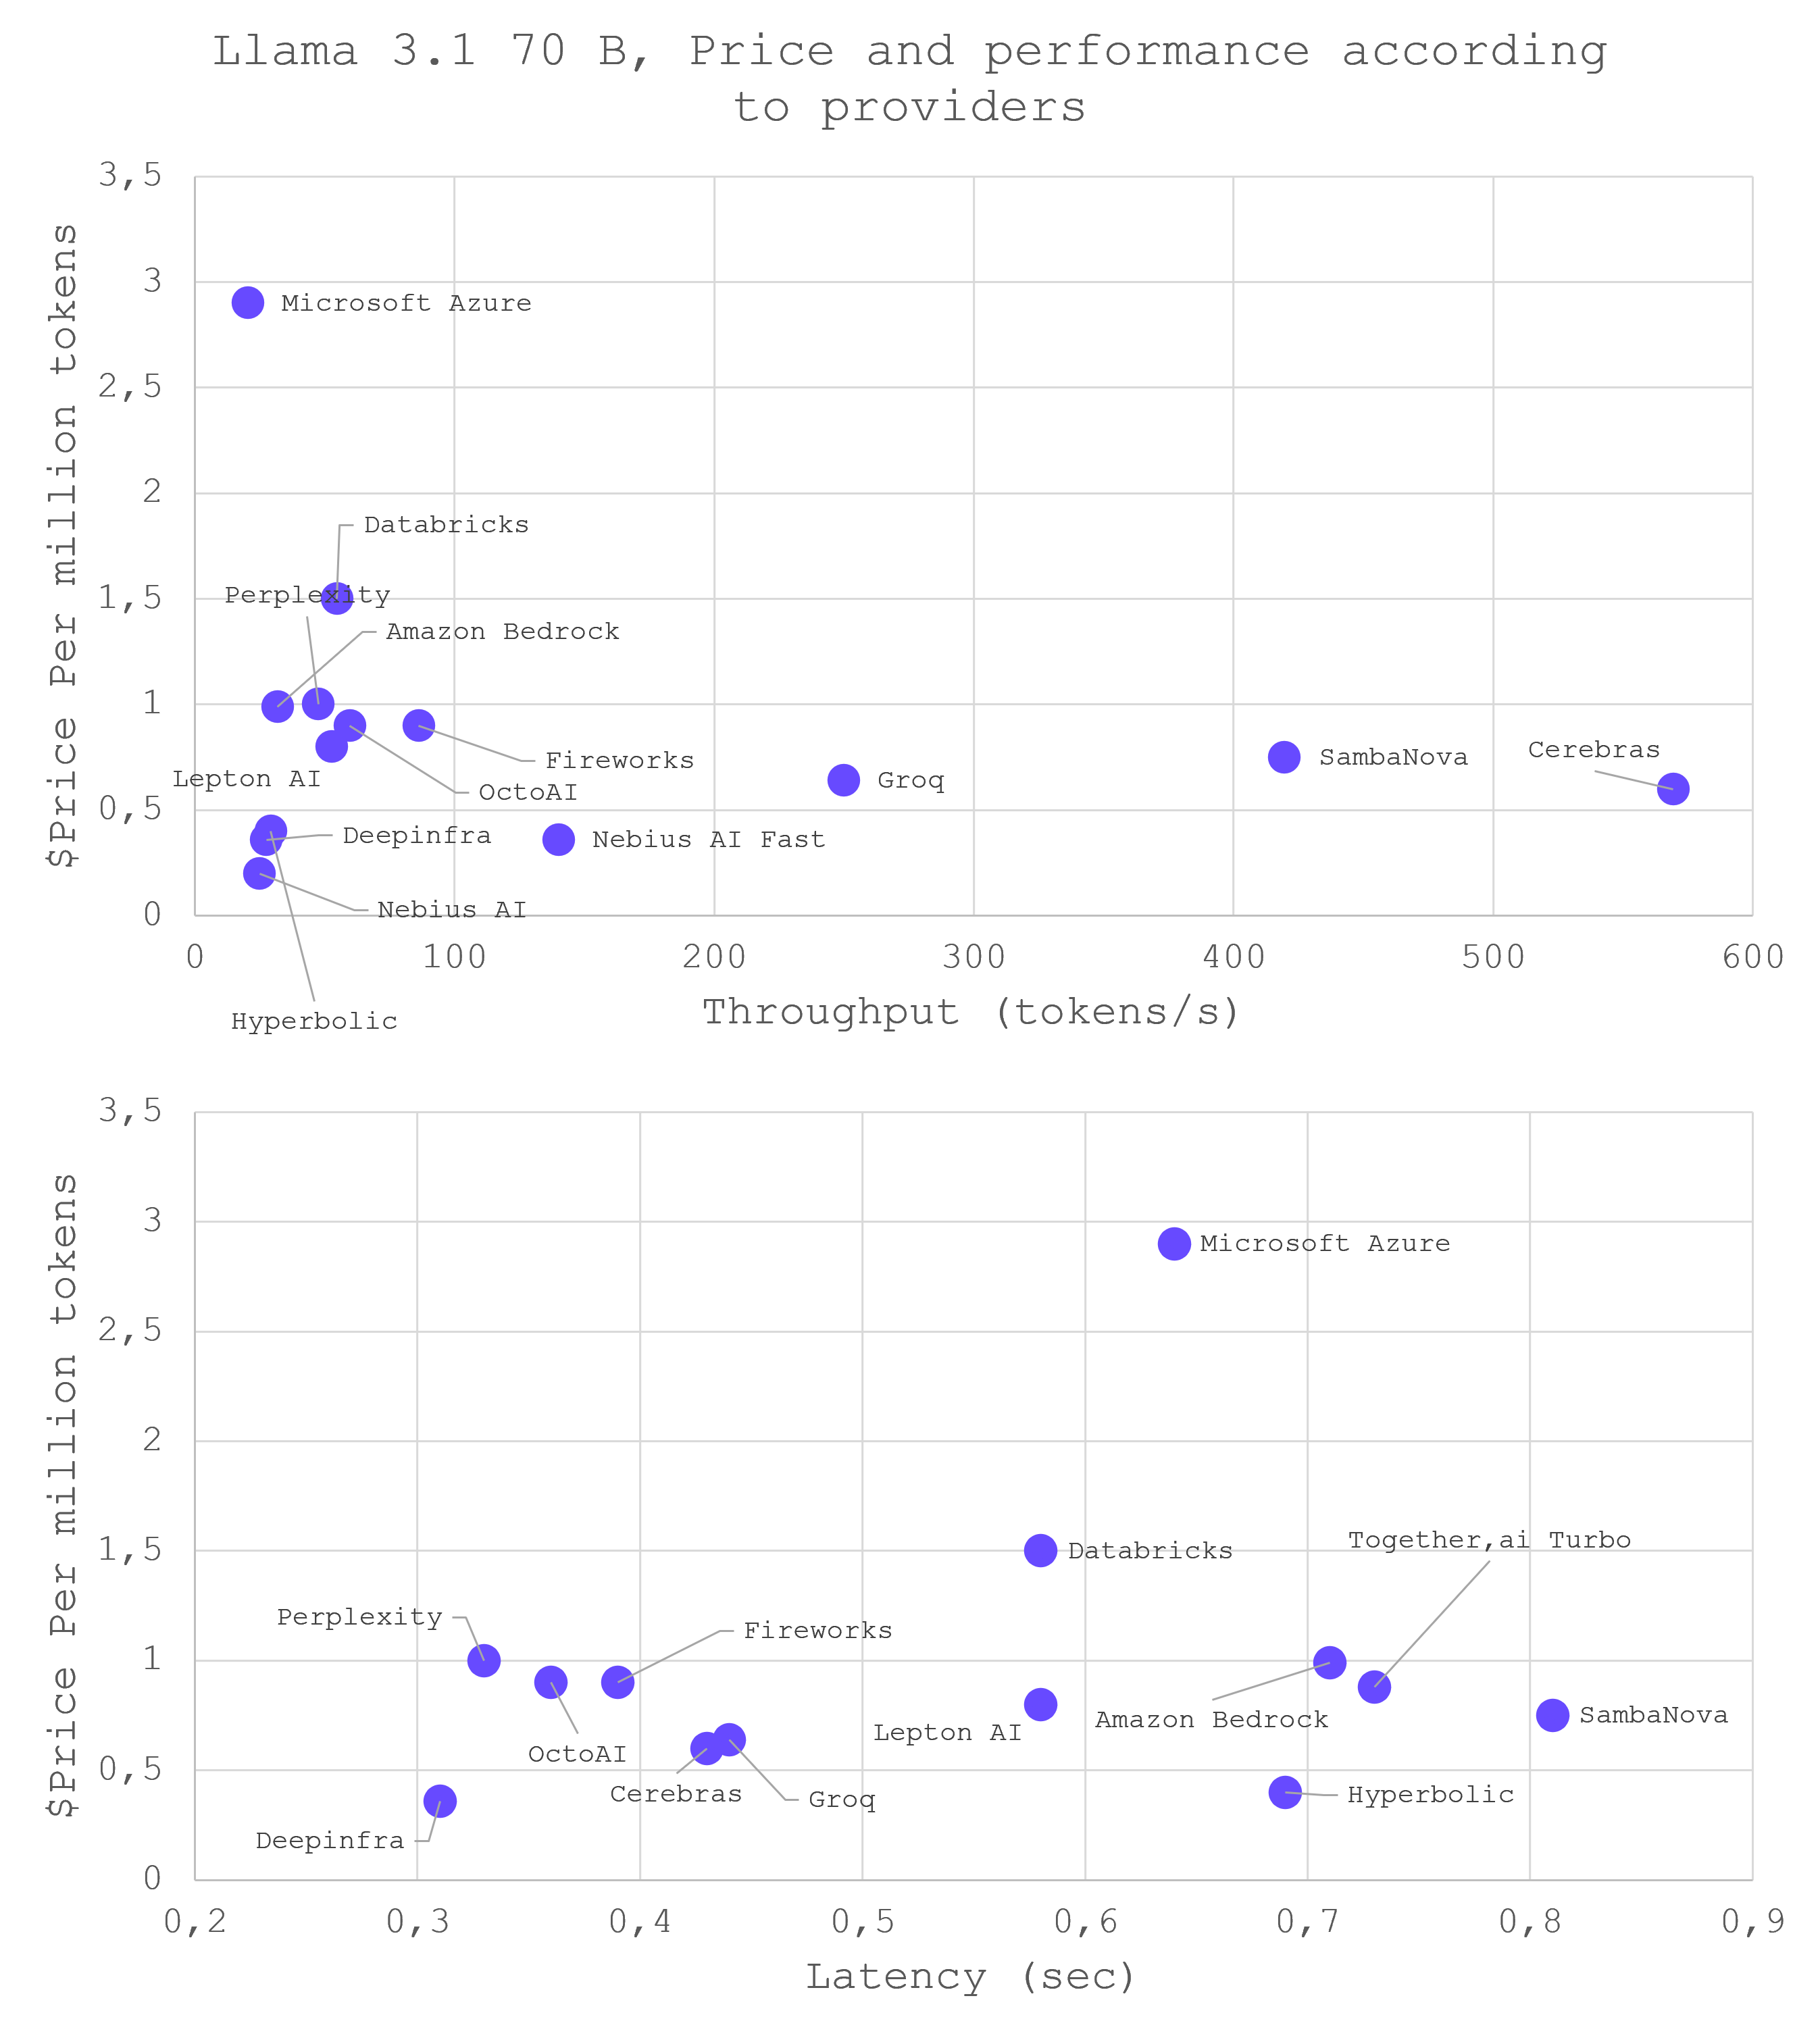
\includegraphics[width=0.85\textwidth]{images/relation_price_performance_provider_llama3.1_70b.png}
    \caption{Price vs. performance for Llama 3.1 70B across providers (no clear correlation).}
    \label{fig:price_performance_llama}
\end{figure}

We envisioned an intermediary layer capable of routing LLM requests dynamically across providers, optimizing either for speed, price, or a combination of both, according to user preferences.
In other words, rather than forcing developers to choose and maintain multiple providers manually, Makehub would serve as a unified API endpoint, handling the complexity of real-time optimization in the background.

\medskip

\noindent\textbf{From market observation to technical problem.}
The observations made during our Berkeley immersion crystallized into a clear problem statement. The LLM provider market exhibits three structural inefficiencies that create both developer pain and entrepreneurial opportunity:

\begin{enumerate}
\item \textbf{Fragmentation and opacity.} With over 20 providers offering overlapping model catalogs, developers face an overwhelming decision space with no standardized benchmarks or service-level agreements. The market lacks transparency: performance metrics are not publicly disclosed, and pricing structures vary wildly (per-token, per-request, tiered subscriptions).

\item \textbf{Spatial and temporal volatility.} Even when a developer selects a provider, performance is not constant. The same model hosted by different providers yields drastically different throughput and latency depending on infrastructure quality, geographic routing, and batching strategies. Furthermore, a single provider's performance fluctuates across hours due to varying load (as we will document empirically in §3.1). This dual volatility—across providers and across time—makes rational optimization nearly impossible without continuous monitoring.

\item \textbf{High switching costs and lock-in.} Integrating a new provider requires modifying API endpoints, managing separate credentials, and adapting to provider-specific quirks (e.g., differing error codes, rate-limiting schemes, authentication flows). These frictions discourage experimentation, leading developers to settle for a single, often suboptimal, provider. Monthly bills of \officialeuro200--1,200 are common, yet many developers remain unaware that equivalent performance could be obtained at 30--50\% lower cost by switching providers—or that their current provider is underperforming relative to competitors.
\end{enumerate}

\medskip

\noindent\textbf{The core technical challenge.}
These market inefficiencies give rise to a concrete optimization problem: \emph{how can LLM requests be routed, in real time, to the provider that maximizes a user-defined objective function balancing cost, performance, and reliability?}

This problem sits at the intersection of \textbf{distributed systems} (monitoring heterogeneous APIs, handling fallbacks), \textbf{real-time optimization} (routing decisions under uncertainty with millisecond latency budgets), and \textbf{economic modeling} (reconciling volatile pricing with performance trade-offs). Solving it requires:
\begin{itemize}
    \item \textbf{Continuous measurement}: Passive instrumentation of production traffic to track provider performance in real time (§3.2).
    \item \textbf{Multi-dimensional scoring}: A vectorial optimization algorithm that synthesizes latency, throughput, cost, and user preferences into routing decisions (§5.2).
    \item \textbf{Provider abstraction}: A unified API that hides heterogeneity while preserving full functionality (streaming, tool calling, etc.), enabling seamless provider switching (§3.1).
    \item \textbf{Robustness and fallback}: Graceful handling of provider failures, rate limits, and degraded performance through cascading retry logic (§5.3).
\end{itemize}

\medskip

\noindent This realization—that developer pain stemmed from a solvable systems and optimization challenge rather than fundamental model limitations—marked the true genesis of Makehub. Our value proposition is not to build better models, but to build \textbf{better infrastructure} for accessing them: a routing layer that brings transparency, efficiency, and cost savings to an otherwise opaque and inefficient market. The remainder of this thesis documents how we translated this vision into a production system serving 170,000+ requests across 20+ providers.


% ==========================

\newpage
\section{Problem Statement: Optimizing LLM Request Routing}
\subsection{Definition of the protocol used for LLM calls}

This subsection explains what happens during an LLM call from a systems perspective and how requests are encoded over HTTP. We use OpenAI's \emph{Chat Completions} as a reference surface, then cover streaming and tool/function calling with a concrete, end-to-end weather example.

\subsubsection{High-level picture}

A client (e.g., a code assistant) sends a prompt to a provider hosting a model; the provider returns an answer, often streamed token-by-token.

\begin{quote}\itshape
Client: ``Hello.'' \\
Server: ``Hello, how are you?''
\end{quote}

Two capabilities are essential in real applications:
\begin{enumerate}
  \item \textbf{Streaming} so the UI updates as tokens arrive.
  \item \textbf{Tool calling} so the model can request a function call (e.g., weather) before finalizing the answer.
\end{enumerate}

\subsubsection{HTTP method, base URL, and model}

Inference uses a standard \texttt{HTTP POST} to the provider's REST endpoint. Developers control:
\begin{itemize}
  \item the \textbf{base URL}, e.g., \texttt{https://api.openai.com/v1/} (or a compatible proxy); and
  \item the \textbf{model} identifier, e.g., \texttt{gpt-4o}.
\end{itemize}
Changing either lets you switch provider or model with minimal code changes. This is a key lever for Makehub's routing approach.

\subsubsection{Minimal text-only call (non-streaming)}

\noindent\textbf{What this request does.}
It sends a single user message (\texttt{"Hello"}) to the chat completions endpoint. The server returns a JSON response containing the assistant's message plus metadata (IDs, token usage, etc.).

\begin{listing}[H]
\begin{minted}{text}
# Request
POST https://api.openai.com/v1/chat/completions
Authorization: Bearer $OPENAI_API_KEY
Content-Type: application/json
\end{minted}
\begin{minted}{json}
{
  "model": "gpt-4o",
  "messages": [
    {"role": "user", "content": "Hello"}
  ]
}
\end{minted}
\caption{cURL request and minimal JSON body (Chat Completions)}
\end{listing}

\noindent\textbf{Key fields.}
\texttt{model} selects the target model. \texttt{messages} is an ordered list of chat turns; at minimum, a user turn. Optional fields (not shown) include \texttt{temperature}, \texttt{max\_tokens}, \texttt{stop}, etc.

\begin{listing}[H]
\begin{minted}{json}
{
  "id": "chatcmpl-abc123",
  "created": 1730000000,
  "model": "gpt-4o",
  "choices": [
    {
      "index": 0,
      "finish_reason": "stop",
      "message": {
        "role": "assistant",
        "content": "Hello, how are you?"
      }
    }
  ],
  "usage": { "prompt_tokens": 2, "completion_tokens": 5, "total_tokens": 7 }
}
\end{minted}
\caption{Illustrative response (trimmed)}
\end{listing}

\noindent\textbf{How to read the response.}
The JSON response contains several critical fields for both extracting the model's output and monitoring resource consumption:

\begin{itemize}
    \item \textbf{\texttt{choices[0].message.content}}: This is the core payload—the assistant's natural-language answer. The \texttt{choices} array allows the API to support multiple completions per request (though most use cases set \texttt{n=1}, yielding a single choice at index 0). The \texttt{message} object follows the same structure as the input \texttt{messages} array: a \texttt{role} (always \texttt{"assistant"} in the response) and \texttt{content} (the generated text).

    \item \textbf{\texttt{usage}}: This object provides token-level accounting, essential for cost tracking and billing. It contains three counters:
    \begin{itemize}
        \item \texttt{prompt\_tokens}: The number of tokens in the input (user messages, system prompt, context).
        \item \texttt{completion\_tokens}: The number of tokens generated by the model.
        \item \texttt{total\_tokens}: The sum of \texttt{prompt\_tokens} and \texttt{completion\_tokens}.
    \end{itemize}
    Since most providers charge separately for input and output tokens (e.g., OpenAI's GPT-4o costs \$2.50 per million input tokens and \$10.00 per million output tokens as of January 2025), the \texttt{usage} object is indispensable for real-time cost calculation. For example, a request with 1,000 prompt tokens and 500 completion tokens would cost: $(1000 \times 2.50 + 500 \times 10.00) / 1{,}000{,}000 = \$0.0075$.

    \item \textbf{\texttt{finish\_reason}}: This field indicates \emph{why} the generation terminated, which is critical for handling edge cases and debugging:
    \begin{itemize}
        \item \texttt{"stop"}: The model reached a natural stopping point (e.g., completed a sentence, emitted an end-of-turn token). This is the expected outcome for most requests.
        \item \texttt{"length"}: Generation was truncated because the output exceeded the model's maximum token limit or the user-specified \texttt{max\_tokens} parameter. In this case, \texttt{content} may be incomplete (e.g., a code snippet cut off mid-function). Clients should detect this and either increase \texttt{max\_tokens} or prompt the user to continue.
        \item \texttt{"tool\_calls"}: The model invoked a function/tool (see §3.1.4). The \texttt{content} field will be \texttt{null}, and instead, \texttt{message.tool\_calls} will contain structured function call requests that the client must execute.
        \item \texttt{"content\_filter"} (provider-specific): Some providers (e.g., Azure OpenAI) apply content moderation filters. If the output violates policy (e.g., generates harmful content), the request is aborted and \texttt{finish\_reason} is set to \texttt{"content\_filter"}. Clients must handle this gracefully, typically by informing the user and avoiding retry loops.
    \end{itemize}
\end{itemize}

\medskip

\noindent\textbf{Practical implications for Makehub.}
When routing requests across providers, Makehub must normalize these response structures. While the OpenAI format is widely adopted (Anthropic, Mistral, and many others follow it closely), subtle differences exist:
\begin{itemize}
    \item Some providers omit the \texttt{usage} object in streaming mode, requiring Makehub to count tokens client-side using a tokenizer (e.g., \texttt{tiktoken} for OpenAI models).
    \item \texttt{finish\_reason} values are not fully standardized. For instance, some providers use \texttt{"stop"} while others use \texttt{"end\_turn"} or \texttt{"eos\_token"}. Makehub's provider adapters (§5.1.3) translate these into a canonical representation.
    \item The \texttt{id} and \texttt{created} timestamp are provider-generated and serve as idempotency keys. Makehub logs these for request tracing and debugging but does not expose them directly to end users.
\end{itemize}

\subsubsection{Streaming with Server-Sent Events (SSE)}

\noindent\textbf{What this does.}
Setting \texttt{"stream": true} in the request makes the server emit a sequence of SSE frames. Each frame contains a \texttt{delta} (partial text or metadata). The stream ends with \texttt{[DONE]}. This yields responsive UIs without waiting for the full completion.

\begin{listing}[H]
\begin{minted}{text}
data: {"id":"chatcmpl-...","choices":[{"delta":{"role":"assistant"}}]}
data: {"id":"chatcmpl-...","choices":[{"delta":{"content":"Hello"}}]}
data: {"id":"chatcmpl-...","choices":[{"delta":{"content":", how are"}}]}
data: {"id":"chatcmpl-...","choices":[{"delta":{"content":" you?"}}]}
data: [DONE]
\end{minted}
\caption{Conceptual SSE frames (illustrative)}
\end{listing}

\noindent\textbf{Client responsibilities.}
Append each \texttt{delta.content} to your UI buffer in order. Handle edge cases: empty deltas (role only), multiline chunks, and the terminal \texttt{[DONE]}. If a network error occurs mid-stream, degrade gracefully (e.g., retry without losing already-rendered text).

\subsubsection{Tool (function) calling with a weather example}

\noindent\textbf{Why tools.}
The model sometimes needs fresh or external data (e.g., weather, internal APIs, databases). Tool calling lets the model request a structured function call; \emph{the client} executes that function and returns the result so the model can finalize its answer.

Tools are particularly essential in code assistants because these systems must interact with the development environment: executing commands, reading and modifying files, accessing the file system, searching through code, or running tests. Without these external interaction capabilities, a code assistant would be limited to generating text without being able to verify, test, or deploy the solutions it proposes.

\paragraph{Step 1: declare the tool and ask a question}

\noindent\textbf{What this request does.}
We declare a function (\texttt{get\_current\_weather}) via JSON Schema in \texttt{tools}. The user asks about the weather in Paris. The model is now allowed to call this function if it deems it useful.

\begin{listing}[H]
\begin{minted}{text}
POST https://api.openai.com/v1/chat/completions
Authorization: Bearer $OPENAI_API_KEY
Content-Type: application/json
\end{minted}
\begin{minted}{json}
{
  "model": "gpt-4o",
  "messages": [
    {"role": "user", "content": "What's the weather in Paris right now?"}
  ],
  "tools": [
    {
      "type": "function",
      "function": {
        "name": "get_current_weather",
        "description": "Get the current weather in a city",
        "parameters": {
          "type": "object",
          "properties": {
            "city":  { "type": "string" },
            "units": { "type": "string", "enum": ["metric","imperial"] }
          },
          "required": ["city"]
        }
      }
    }
  ]
}
\end{minted}
\caption{Request with a tool declaration}
\end{listing}

\noindent\textbf{Key fields.}
\texttt{tools[*].function.name} is the unique function identifier the model will reference. \texttt{parameters} defines a strict JSON Schema so the model knows valid argument names and types.

\noindent\textbf{Tool schema structure.}
The tool declaration follows a structured format where each tool has a \texttt{type} (always \texttt{"function"} for function calls) and a \texttt{function} object containing:
\begin{itemize}
  \item \texttt{name}: A descriptive identifier that the model will use to reference this function
  \item \texttt{description}: A clear explanation of what the function does, helping the model decide when to call it
  \item \texttt{parameters}: A JSON Schema object defining the function's input structure, including:
    \begin{itemize}
      \item \texttt{type}: Usually \texttt{"object"} for structured parameters
      \item \texttt{properties}: Each parameter with its type (\texttt{string}, \texttt{number}, \texttt{boolean}, etc.)
      \item \texttt{required}: Array listing which parameters are mandatory
      \item \texttt{enum}: For parameters with restricted values (like \texttt{["metric","imperial"]})
    \end{itemize}
\end{itemize}
This schema acts as a contract between the model and the client, ensuring type safety and enabling the model to generate valid function calls.

\paragraph{Step 2: the model returns a tool call (client must parse it)}

\noindent\textbf{What this means.}
The assistant message includes a \texttt{tool\_calls} array with a function name and serialized \texttt{arguments} (a JSON string). \emph{This is not the final answer.} The client must detect this, execute the function, and then send back a \texttt{role:"tool"} message with the result.

\begin{listing}[H]
\begin{minted}{json}
{
  "choices": [
    {
      "message": {
        "role": "assistant",
        "tool_calls": [
          {
            "id": "call_123",
            "type": "function",
            "function": {
              "name": "get_current_weather",
              "arguments": "{\"city\":\"Paris\",\"units\":\"metric\"}"
            }
          }
        ]
      },
      "finish_reason": "tool_calls"
    }
  ]
}
\end{minted}
\caption{Assistant message requesting a tool call}
\end{listing}

\noindent\textbf{Client responsibilities.}
\begin{itemize}
  \item Parse \texttt{arguments} (string) into JSON.
  \item Call your implementation of \texttt{get\_current\_weather(city, units)}.
  \item Capture the tool output (e.g., \texttt{\{"tempC": 25, "condition": "Sunny"\}}).
\end{itemize}

\paragraph{Step 3: send the tool result, then get the final answer}

\noindent\textbf{What this request does.}
We provide the tool output back to the model as a new message with \texttt{role:"tool"} and a \texttt{tool\_call\_id} that matches the earlier call. The model can now incorporate the tool result and produce the final natural-language message.

\begin{listing}[H]
\begin{minted}{text}
POST https://api.openai.com/v1/chat/completions
Authorization: Bearer $OPENAI_API_KEY
Content-Type: application/json
\end{minted}
\caption{HTTP request (endpoint and headers)}
\end{listing}

\begin{listing}[H]
\begin{minted}{json}
{
    "model": "gpt-4o",
    "messages": [
        { "role": "user", "content": "What's the weather in Paris right now?" },
        {
            "role": "assistant",
            "tool_calls": [
                {
                    "id": "call_123",
                    "type": "function",
                    "function": {
                        "name": "get_current_weather",
                        "arguments": "{\"city\":\"Paris\",\"units\":\"metric\"}"
                    }
                }
            ]
        },
        {
            "role": "tool",
            "tool_call_id": "call_123",
            "content": "{\"tempC\":25,\"condition\":\"Sunny\"}"
        }
    ]
}
\end{minted}
\caption{JSON body including the tool result to finalize the request}
\end{listing}

\noindent\textbf{Expected final response.}
The server now returns a regular assistant message, e.g.:

\begin{listing}[H]
\begin{minted}{json}
{
  "choices": [
    {
      "message": {
        "role": "assistant",
        "content": "It is currently 25\textdegree C and sunny in Paris."
      },
      "finish_reason": "stop"
    }
  ]
}
\end{minted}
\caption{Final assistant message (trimmed)}
\end{listing}


\subsubsection{What varies across providers (and why Makehub abstracts it)}

The round-trip is conceptually the same across providers, but field names, envelopes, and authentication methods differ:
\begin{description}
  \item[Anthropic (Claude).] Tool use appears as \texttt{tool\_use} content blocks; clients must reply with \texttt{tool\_result} blocks before Claude continues. Roles and message shapes differ from Chat Completions.
  \item[Google Gemini.] The model emits function calls and expects function responses (and the Live API has dedicated tool-response mechanics). Field names differ from OpenAI's.
  \item[Azure OpenAI.] While using OpenAI models, Azure requires different authentication (API keys tied to Azure subscriptions rather than OpenAI accounts) and uses Azure-specific endpoints with different URL patterns (\texttt{https://\{resource\}.openai.azure.com/}).
\end{description}

These differences justify a compatibility layer. Makehub exposes an OpenAI-compatible surface (same request/response shape for developers) and normalizes provider-specific details internally. This minimizes switching costs (change base URL and/or model) and enables dynamic routing based on cost/performance without application rewrites.



\subsection{State of the Art: Industry Methods for Cost/Performance Optimization}

Before delving into Makehub's specific monitoring and routing implementation, it is useful to situate the project within the broader landscape of optimization strategies currently employed in the LLM inference industry. This section surveys four complementary approaches that address cost and performance trade-offs: server optimization, model routing, prompt compression, and prompt caching. While Makehub primarily focuses on server optimization (selecting the best provider for a given model), understanding these alternative techniques is essential both for contextualizing our contribution and for identifying opportunities for future integration.

\subsubsection{Server optimization}

Server optimization, also known as \textbf{provider arbitrage} or \textbf{dynamic routing}, is the most direct approach to reducing inference costs while maintaining or improving performance. The core idea is straightforward: for a given model (e.g., Mistral-7B-Instruct or Claude 3.5 Sonnet), multiple providers may offer hosting services, each with different pricing structures and real-time performance characteristics. By intelligently selecting the provider at request time, substantial cost savings and latency improvements become possible.

\paragraph{The fragmentation of the open-source hosting market.}

This optimization opportunity arises primarily in the context of \textbf{open-source models}, where the weights are publicly available and any infrastructure provider can host them. For closed-source models (e.g., GPT-4, Claude), access is typically restricted to a single vendor or a small set of authorized partners (e.g., Azure OpenAI Service, AWS Bedrock for Claude), leaving limited room for provider arbitrage—though geographic routing and regional pricing variations can still be exploited.

In contrast, open-source models such as Meta's LLaMA family, Mistral AI's models, and others have spawned a competitive hosting ecosystem. Providers such as \textbf{Together AI}, \textbf{Replicate}, \textbf{SambaNova}, \textbf{Fireworks AI}, and \textbf{Anyscale} all offer inference APIs for the same underlying models, but with significant differences in:
\begin{itemize}
    \item \textbf{Pricing per million tokens}: costs can vary by a factor of 2--5× for identical models.
    \item \textbf{Throughput and latency}: depending on hardware (GPU type, batching strategy), geographic proximity, and current load, response times fluctuate substantially.
    \item \textbf{Availability and rate limits}: smaller providers may experience capacity constraints during peak hours, while larger providers offer more stable uptime but at a premium.
\end{itemize}

\paragraph{The absence of price–performance correlation.}

A key empirical finding—one that directly motivated the Makehub project—is that \textbf{there is no consistent correlation between price and performance across providers}. To validate this hypothesis, we analyzed 170,555 real production requests processed through the Makehub platform between April and December 2024, covering GPT-4o, Claude 3.5 Sonnet, and Gemini 2.0 Flash across multiple providers.

Figure~\ref{fig:cost_performance_comparison} presents a comparative analysis of the three most-used models in our production dataset. The data reveals substantial cost–performance disparities: Gemini 2.0 Flash offers a \textbf{37.5× cost advantage} over Claude 3.5 Sonnet while delivering \textbf{16× higher median throughput}. GPT-4o occupies a middle position, with balanced latency but higher cost than Gemini. Critically, these differences are not explained by performance trade-offs—Gemini is simultaneously cheaper \emph{and} faster than Claude for most workloads.

\begin{figure}[H]
\centering
\includegraphics[width=0.9\textwidth]{DataAnalysisCorrelation/figure_cost_performance.png}
\caption{Cost vs. performance for the three most-used models (170,555 production requests).}
\label{fig:cost_performance_comparison}
\end{figure}

This lack of correlation is explained by several factors:
\begin{itemize}
    \item \textbf{Varying hardware and optimization stacks}: providers use different GPU types (A100, H100, custom ASICs) and inference frameworks (vLLM, TensorRT-LLM, custom kernels), each with distinct throughput profiles.
    \item \textbf{Dynamic load balancing}: a provider experiencing high demand at time $t$ will exhibit degraded throughput, even if it is nominally faster during off-peak hours.
    \item \textbf{Pricing opacity}: inference pricing is not purely cost-based; it reflects strategic positioning, early-adopter subsidies, and margin targets. For example, preliminary research suggests that some providers (e.g., Together AI) operate with margins as high as 70--80\% above raw compute costs, while others compete more aggressively on price.
\end{itemize}

\paragraph{The developer's challenge.}

For an individual developer or organization, exploiting this fragmentation manually is impractical. Effective provider arbitrage would require:
\begin{enumerate}
    \item \textbf{Maintaining accounts and credits with all relevant providers}, which introduces financial overhead and complexity.
    \item \textbf{Monitoring real-time performance across providers}, necessitating continuous benchmarking infrastructure.
    \item \textbf{Switching API endpoints and credentials dynamically}, which is error-prone and disrupts workflow integration.
    \item \textbf{Understanding pricing nuances}, including per-token costs, prompt caching discounts, and regional variations.
\end{enumerate}

In practice, developers typically settle for a single provider, absorbing inefficiencies in exchange for simplicity. This inertia is precisely what Makehub aims to overcome.

\paragraph{Makehub's value proposition: transparent provider routing.}

Makehub addresses this problem by acting as a \textbf{unified API gateway}. Developers interact with a single endpoint compatible with the OpenAI Chat Completions standard, specifying only:
\begin{itemize}
    \item the desired \textbf{model} (e.g., \texttt{mistralai/Mistral-7B-Instruct-v0.2}), and
    \item optionally, a routing preference: \textbf{minimize cost}, \textbf{maximize speed}, or \textbf{optimize for a cost/speed ratio}.
\end{itemize}

Behind the scenes, Makehub:
\begin{enumerate}
    \item Maintains authenticated connections to all major providers.
    \item Continuously monitors real-time latency and throughput for each model–provider pair (as described in Section~3).
    \item Routes each request to the provider offering the best trade-off according to the user's specified criteria.
    \item Abstracts away protocol differences (e.g., Anthropic's message format vs. OpenAI's) so that responses are always returned in a consistent format.
\end{enumerate}

This approach transforms provider arbitrage from an impractical manual task into an automated, zero-configuration optimization. By aggregating demand across multiple users, Makehub also achieves economies of scale in monitoring and account management, making real-time routing feasible even for small teams and individual developers.

\paragraph{Limitations and complementarity with other techniques.}

Server optimization is powerful but inherently limited by the capabilities of the selected model. If a developer chooses a large, expensive model (e.g., GPT-4) for a simple task, even optimal provider selection cannot reduce costs below a certain threshold. This is where complementary techniques—\textbf{model routing} (§2.2.2), \textbf{prompt compression} (§2.2.3), and \textbf{prompt caching} (§2.2.4)—become essential. These methods reduce the computational burden itself, rather than merely optimizing where it is executed. In the long term, Makehub envisions integrating all four strategies into a unified optimization framework, but the initial focus remains on provider-level arbitrage due to its immediate, measurable impact.


\subsubsection{Model routing}

While server optimization focuses on selecting the best \emph{provider} for a given model, \textbf{model routing} takes a complementary approach: selecting the best \emph{model} for a given task. The core insight is that not all user requests require the same level of reasoning capability. Simple queries (e.g., formatting code, answering factual questions) can often be handled by smaller, cheaper, and faster models, while complex tasks (e.g., multi-step reasoning, algorithmic problem-solving) benefit from larger, more capable—but more expensive—models. By dynamically routing requests to appropriately-sized models, significant cost reductions can be achieved without sacrificing output quality.

\paragraph{The cost–capability spectrum.}

LLMs exist along a spectrum of capability and cost. At one extreme, large frontier models such as OpenAI o1, Claude Sonnet 4, and Gemini 2.0 Pro offer state-of-the-art reasoning and generation quality, but at a premium price (often \$10--\$60 per million input tokens for reasoning-intensive models). At the other extreme, smaller models such as DeepSeek-V3, Claude 3.5 Haiku, Mistral Codestral (formerly Devstral), and DeepSeek-R1-Distill provide adequate performance for many tasks at a fraction of the cost (\$0.10--\$2 per million tokens).

The key observation is that \textbf{request complexity varies widely}. In the context of code assistants, for example:
\begin{itemize}
    \item \textbf{Simple requests}: "Format this JSON," "Add comments to this function," "What does this error mean?" → A small model suffices.
    \item \textbf{Moderate requests}: "Refactor this module to use async/await," "Write unit tests for this class" → A mid-sized model is appropriate.
    \item \textbf{Complex requests}: "Design a distributed caching layer with Redis and implement it," "Debug this concurrency issue in a multi-threaded application" → A large, capable model is necessary.
\end{itemize}

By routing simple requests to cheaper models and reserving expensive models for complex tasks, a code assistant can reduce average inference costs by 50--80\% while maintaining comparable output quality.

\paragraph{Methods for assessing request complexity.}

The challenge of model routing lies in \textbf{accurately predicting task complexity} before generation. Several approaches have emerged in both research and industry:

\begin{enumerate}
    \item \textbf{Rule-based heuristics.} Simple rules based on request metadata can provide a coarse classification:
    \begin{itemize}
        \item Short prompts ($<$100 tokens) with no code context → likely simple.
        \item Requests containing keywords like "design," "architecture," "debug," "optimize" → likely complex.
        \item Requests referencing multiple files or large codebases → likely complex.
    \end{itemize}
    While easy to implement, rule-based systems lack nuance and are prone to misclassification.

    \item \textbf{Embedding-based similarity (RAG).} Retrieval-Augmented Generation (RAG) techniques can be repurposed for complexity estimation. A reference dataset is constructed with labeled examples:
    \begin{itemize}
        \item \textbf{Complex queries}: e.g., "Implement a custom authentication middleware with JWT and refresh tokens."
        \item \textbf{Simple queries}: e.g., "Fix the indentation in this Python file."
    \end{itemize}
    Each incoming request is embedded (using a model such as \texttt{text-embedding-ada-002} or an open-source alternative), and its cosine similarity to the reference sets is computed. Requests closer to the "complex" cluster are routed to larger models.

    This approach is more robust than heuristics, as it captures semantic similarity, but requires careful curation of the reference dataset and incurs a small embedding cost per request.

    \item \textbf{LLM-as-a-Judge.} A third approach—increasingly popular in production systems—uses a \textbf{small, fast LLM to evaluate the complexity of the incoming request}. For example, a lightweight model such as Mistral 7B or GPT-3.5 Turbo is prompted:

    \begin{quote}
    \textit{``You are a classifier. Rate the complexity of the following coding task on a scale from 1 (trivial) to 10 (highly complex). Consider factors such as: number of steps required, need for external knowledge, algorithmic reasoning, and ambiguity. Respond with only a number.''}
    \end{quote}

    The classifier's output (e.g., 3, 7, 9) is then mapped to a model tier:
    \begin{itemize}
        \item Complexity 1--4 → Small model (e.g., DeepSeek-V3, Mistral Codestral, Claude 3.5 Haiku)
        \item Complexity 5--7 → Medium model (e.g., Claude Sonnet 4, GPT-4o, DeepSeek-R1-Distill)
        \item Complexity 8--10 → Large model (e.g., OpenAI o1, Claude Sonnet 4, DeepSeek-R1)
    \end{itemize}

    This method is flexible and adapts naturally to new types of tasks, but it introduces a small latency overhead (typically 200--500ms for the classification call) and a marginal cost for the classifier model itself.
\end{enumerate}

\paragraph{Example: three-tier model routing strategy.}

Table~\ref{tab:model_routing_tiers} illustrates a concrete model routing strategy that could be deployed in a code assistant like Cursor or Cline.

\begin{table}[H]
\centering
\caption{Example three-tier model routing strategy based on complexity score.}
\label{tab:model_routing_tiers}
\begin{tabular}{|c|l|l|r|}
\hline
\textbf{Complexity} & \textbf{Model tier} & \textbf{Example model} & \textbf{Cost (per 1M tokens)} \\
\hline
1--4 & Small, fast & DeepSeek-V3 & \$0.27 (input), \$1.10 (output) \\
     &             & Mistral Codestral & \$0.30 \\
     &             & Claude 3.5 Haiku & \$0.25 (input), \$1.25 (output) \\
\hline
5--7 & Medium & Claude Sonnet 4 & \$3.00 (input), \$15.00 (output) \\
     &        & GPT-4o & \$2.50 (input), \$10.00 (output) \\
     &        & DeepSeek-R1-Distill & \$0.55 (input), \$2.19 (output) \\
\hline
8--10 & Large, capable & OpenAI o1 & \$15.00 (input), \$60.00 (output) \\
      &                & Claude Sonnet 4 & \$3.00 (input), \$15.00 (output) \\
      &                & DeepSeek-R1 & \$2.19 (input), \$8.19 (output) \\
\hline
\end{tabular}
\end{table}

By routing 60\% of requests to tier 1, 30\% to tier 2, and 10\% to tier 3, a typical code assistant could reduce its average cost per request by 70\% compared to using a frontier model for all requests.

\paragraph{Real-world adoption: Cursor and other assistants.}

Model routing is not merely a theoretical optimization—it is actively deployed by leading code assistants. \textbf{Cursor}, for example, is known to employ dynamic model selection based on task complexity, though the exact algorithm is proprietary. Anecdotal evidence from user reports suggests that Cursor defaults to smaller models (e.g., Claude 3.5 Haiku, DeepSeek-V3) for simple completions and escalates to Claude Sonnet 4 or OpenAI o1 for complex reasoning tasks.

This strategy is economically essential for assistants offering "unlimited" plans (e.g., Cursor's \$20/month tier, Claude Code's \$200/month enterprise tier): without model routing, heavy users would generate unsustainable costs. By reserving expensive models for genuinely complex tasks, these platforms can offer flat-rate pricing while maintaining profitability.

\paragraph{Challenges and limitations.}

Model routing introduces several trade-offs:
\begin{itemize}
    \item \textbf{Latency overhead}: Classification (whether via embedding or LLM-as-a-Judge) adds 100--500ms before generation begins, which may be noticeable in interactive settings.
    \item \textbf{Misclassification risk}: A request incorrectly routed to a small model may produce low-quality output, frustrating users. Conversely, over-routing to large models negates cost savings.
    \item \textbf{Model capability drift}: As models evolve (e.g., Claude 3.5 Sonnet vs. Claude Sonnet 4, GPT-4o vs. o1, DeepSeek-V3 vs. DeepSeek-R1), the complexity thresholds must be recalibrated to reflect new capability distributions.
\end{itemize}

Despite these challenges, model routing remains one of the most effective cost-reduction techniques available, and it is highly complementary to server optimization. In Makehub's roadmap, model routing is a natural next step after provider arbitrage is fully operational.

\paragraph{Integration with Makehub.}

While Makehub's initial focus is on server optimization (routing to the best provider for a given model), the architecture is designed to accommodate model routing in the future. By extending the routing API to accept a complexity hint or allowing Makehub to perform its own complexity classification, users could benefit from both provider arbitrage \emph{and} model selection simultaneously. For example:
\begin{itemize}
    \item A simple request classified as complexity 3 could be routed to \textbf{DeepSeek-V3 on the cheapest available provider}.
    \item A complex request classified as complexity 9 could be routed to \textbf{Claude Sonnet 4 or DeepSeek-R1 on the fastest available provider}.
\end{itemize}

This dual-layer optimization—model selection \emph{and} provider selection—represents the long-term vision for Makehub's routing intelligence.


\subsubsection{Prompt compression}

Prompt compression addresses a fundamental cost driver in LLM inference: the size of the input context. In code assistants and other agentic systems, prompts often include extensive contextual information—entire codebases, chat histories, documentation snippets—leading to input token counts in the tens or hundreds of thousands. Since pricing is per-token (both input and output), reducing input size directly translates to cost savings. Prompt compression techniques aim to preserve semantic content while minimizing token consumption.

\paragraph{The context explosion problem in code assistants.}

Modern code assistants operate with \textbf{large, multi-turn conversation contexts}. A typical interaction might include:
\begin{itemize}
    \item The user's current question (e.g., "Refactor this authentication module to use OAuth2").
    \item Multiple prior messages in the conversation (previous questions, assistant responses, clarifications).
    \item The content of several files in the codebase (e.g., \texttt{auth.py}, \texttt{config.yaml}, \texttt{routes.js}).
    \item System prompts and tool definitions (instructions on how to use functions, file operations, etc.).
\end{itemize}

This can easily reach 50,000--200,000 input tokens per request. At \$3 per million input tokens (e.g., Claude 3.5 Sonnet), a single request costs \$0.15--\$0.60 just for the input. For a developer making 100 requests per day, this amounts to \$15--\$60 daily, or \$450--\$1,800 per month—purely from input tokens.

Prompt compression seeks to reduce this burden by intelligently \textbf{condensing or filtering the context} while retaining the information necessary for the model to generate a high-quality response.

\paragraph{Method 1: Summarization with a smaller model.}

One approach is to use a \textbf{lightweight, inexpensive model} (e.g., Claude 3.5 Haiku, Mistral Codestral, DeepSeek-V3) to summarize or rephrase verbose context before passing it to a larger, more expensive model.

\textbf{Workflow:}
\begin{enumerate}
    \item The assistant receives a new user query along with a large conversation history (e.g., 20 messages totaling 40,000 tokens).
    \item A small summarization model is prompted:
    \begin{quote}
    \textit{``Summarize the following conversation concisely, preserving key technical details, decisions, and unresolved issues. Omit pleasantries and redundant information.''}
    \end{quote}
    \item The summarized context (now 5,000 tokens) is combined with the current query and sent to the primary model (e.g., Claude Sonnet 4, OpenAI o1, DeepSeek-R1).
\end{enumerate}

\textbf{Cost analysis:}
\begin{itemize}
    \item Original cost (40,000 input tokens at \$3/M for Claude Sonnet 4): \$0.12
    \item Summarization cost (40,000 tokens at \$0.27/M for DeepSeek-V3): \$0.011
    \item Compressed cost (5,000 tokens at \$3/M): \$0.015
    \item \textbf{Total: \$0.026 (78\% savings)}
\end{itemize}

This method works well for conversational context but may lose nuance or omit details that the primary model would have found useful. It is best suited for scenarios where the conversation history is largely informational rather than directly task-critical.

\paragraph{Method 2: Message filtering with LLM-based relevance scoring.}

A more surgical approach is to \textbf{selectively remove irrelevant messages} from the conversation history rather than summarizing everything. This is particularly effective when the current user query pertains to a specific subset of files or topics, rendering earlier messages obsolete.

\textbf{Workflow:}
\begin{enumerate}
    \item The assistant receives a conversation with 15 messages. The latest user query is: "Add input validation to the \texttt{login()} function in \texttt{auth.py}."
    \item A small classifier model evaluates each message for relevance to the current query:
    \begin{quote}
    \textit{``Does the following message provide useful context for the query 'Add input validation to login() in auth.py'? Answer YES or NO.''}
    \end{quote}
    \item Messages about unrelated files (\texttt{database.py}, \texttt{README.md}) or tangential topics (deployment, testing infrastructure) are marked as irrelevant and removed.
    \item The filtered context (now 6 messages instead of 15) is sent to the primary model.
\end{enumerate}

\textbf{Example: message filtering in action.}

Consider the following conversation context:

\begin{listing}[H]
\begin{minted}{json}
[
  {"role": "user", "content": "Show me the database schema in database.py"},
  {"role": "assistant", "content": "[database.py content, 8000 tokens]"},
  {"role": "user", "content": "How do I deploy this app to AWS?"},
  {"role": "assistant", "content": "[deployment instructions, 3000 tokens]"},
  {"role": "user", "content": "Review the auth.py file"},
  {"role": "assistant", "content": "[auth.py content, 5000 tokens]"},
  {"role": "user", "content": "Add input validation to login() in auth.py"}
]
\end{minted}
\caption{Original conversation (simplified)}
\end{listing}

The classifier identifies that messages 1--4 are \textbf{irrelevant} to the current query (which concerns \texttt{auth.py}, not \texttt{database.py} or deployment). After filtering:

\begin{listing}[H]
\begin{minted}{json}
[
  {"role": "user", "content": "Review the auth.py file"},
  {"role": "assistant", "content": "[auth.py content, 5000 tokens]"},
  {"role": "user", "content": "Add input validation to login() in auth.py"}
]
\end{minted}
\caption{Filtered conversation (compressed)}
\end{listing}

This reduces the input from ~16,000 tokens to ~5,000 tokens—a \textbf{69\% reduction}—while preserving all context relevant to the task. The primary model receives cleaner, more focused input, which may even \emph{improve} output quality by reducing noise.

\paragraph{Challenges and trade-offs.}

Prompt compression introduces several considerations:
\begin{itemize}
    \item \textbf{Information loss}: Summarization or filtering may inadvertently discard details that the primary model would have used. This risk can be mitigated by conservative filtering (keeping messages when in doubt) or by hybrid approaches (summarize but retain key excerpts verbatim).
    \item \textbf{Latency overhead}: Both summarization and filtering require an additional LLM call before the main generation, adding 200--500ms. For latency-sensitive applications, this may be unacceptable.
    \item \textbf{Classifier accuracy}: In the filtering approach, a small model may misjudge relevance, leading to critical context being removed. This can be tested and tuned with evaluation datasets.
    \item \textbf{Diminishing returns for short contexts}: If the original context is already small (e.g., 2,000 tokens), compression yields negligible savings and is not worth the overhead.
\end{itemize}

Despite these trade-offs, prompt compression is highly effective for \textbf{long-running, multi-turn conversations} typical of code assistants. By reducing input token counts by 50--80\%, it can halve inference costs without requiring changes to the underlying model or provider.

\paragraph{Complementarity with other techniques.}

Prompt compression is \textbf{orthogonal} to server optimization and model routing:
\begin{itemize}
    \item \textbf{Server optimization} selects the cheapest or fastest provider for a given model—but the input size remains constant.
    \item \textbf{Model routing} selects the cheapest model capable of handling the task—but it still processes the full input.
    \item \textbf{Prompt compression} reduces the input size itself, magnifying the savings from both other techniques.
\end{itemize}

For example, a request compressed from 50,000 tokens to 10,000 tokens enjoys:
\begin{itemize}
    \item 80\% cost reduction on input tokens (direct savings).
    \item Faster inference (smaller inputs → faster processing), benefiting server optimization.
    \item Potential for downgrading to a cheaper model (simpler, focused input may not require frontier-tier reasoning), benefiting model routing.
\end{itemize}

This \textbf{multiplicative effect} makes prompt compression an essential component of a holistic cost optimization strategy.

\paragraph{Integration prospects for Makehub.}

While Makehub's current focus is on provider arbitrage, prompt compression is a natural candidate for future integration. Makehub could offer an optional preprocessing layer:
\begin{enumerate}
    \item User sends a large request (50,000 tokens) to Makehub.
    \item Makehub applies message filtering or summarization (using a cheap classifier model).
    \item The compressed request (10,000 tokens) is routed to the optimal provider.
    \item The user benefits from \textbf{both} compression savings \emph{and} provider optimization.
\end{enumerate}

By exposing a configuration parameter (e.g., \texttt{"enable\_compression": true}), Makehub could allow users to opt into this feature transparently, further reducing their costs without requiring changes to their application logic.


\subsubsection{Prompt caching}

Prompt caching is a provider-side optimization that reduces costs and latency by \textbf{reusing previously computed representations} of input tokens across multiple requests. Unlike the previous techniques (server optimization, model routing, prompt compression), which are implemented client-side or in a routing layer, prompt caching is a feature offered by certain LLM providers—most notably Anthropic (Claude) via both their direct API and AWS Bedrock, and OpenAI (with limited support). When enabled, repeated portions of a prompt are stored in a cache, allowing subsequent requests to skip the expensive re-processing of those tokens.

\paragraph{The redundancy problem in multi-turn conversations.}

In typical code assistant workflows, \textbf{much of the context is repeated across consecutive requests}. Consider a developer working on a refactoring task:
\begin{itemize}
    \item \textbf{Request 1}: "Review the contents of \texttt{auth.py}" → The model receives the full file content (5,000 tokens).
    \item \textbf{Request 2}: "Add input validation to the \texttt{login()} function" → The model again receives the full \texttt{auth.py} content (5,000 tokens) plus the conversation history.
    \item \textbf{Request 3}: "Now add rate limiting" → The model receives \texttt{auth.py}, the previous Q\&A exchanges, and the new query.
\end{itemize}

Without caching, the provider must process the 5,000 tokens of \texttt{auth.py} \emph{from scratch} on every request, even though the file content is identical. This is computationally wasteful and expensive for the user. Prompt caching solves this by storing the internal representation (the "processed" tokens) and reusing it across requests, offering:
\begin{itemize}
    \item \textbf{Cost reduction}: Cached tokens are billed at a fraction of the normal input token price (often 10--20\% of full price).
    \item \textbf{Latency reduction}: Skipping recomputation of cached tokens reduces time-to-first-token, improving responsiveness.
\end{itemize}

\paragraph{How prompt caching works.}

Prompt caching operates at the provider's inference backend. When a request is received:
\begin{enumerate}
    \item The provider computes a \textbf{hash} of specific portions of the input prompt (typically entire messages or designated cache blocks).
    \item If this hash matches a recently used entry in the cache (usually within a 5--10 minute TTL), the provider retrieves the precomputed internal representation instead of reprocessing the tokens.
    \item The cached representation is combined with any new, non-cached tokens, and generation proceeds as usual.
    \item The user is billed at a reduced rate for cached tokens (e.g., \$0.30 per million cached tokens vs. \$3 per million full-price tokens for Claude 3.5 Sonnet).
\end{enumerate}

\textbf{Cache granularity and control:}
\begin{itemize}
    \item \textbf{Anthropic (Claude API and Bedrock)}: Developers explicitly mark messages or content blocks for caching using a \texttt{cache\_control} field. This gives fine-grained control over what is cached.
    \item \textbf{OpenAI}: Caching is mostly automatic and opaque; developers have limited explicit control, though repeated system prompts and large static contexts are cached heuristically.
\end{itemize}

\paragraph{Example: Anthropic's explicit cache control.}

Anthropic's API allows developers to mark specific message blocks for caching. Consider the following request structure:

\begin{listing}[H]
\begin{minted}{json}
{
  "model": "claude-3-5-sonnet-20250219",
  "max_tokens": 1024,
  "system": [
    {
      "type": "text",
      "text": "You are a code assistant. Always provide clear explanations.",
      "cache_control": {"type": "ephemeral"}
    }
  ],
  "messages": [
    {
      "role": "user",
      "content": [
        {
          "type": "text",
          "text": "Here is the auth.py file:\n\n[5000 tokens of code]",
          "cache_control": {"type": "ephemeral"}
        },
        {
          "type": "text",
          "text": "Add input validation to the login() function."
        }
      ]
    }
  ]
}
\end{minted}
\caption{Anthropic request with cache control}
\end{listing}

In this example:
\begin{itemize}
    \item The system prompt and the \texttt{auth.py} file content are marked with \texttt{cache\_control}.
    \item On the first request, these are processed normally and stored in the cache.
    \item On subsequent requests (within the cache TTL), these blocks are retrieved from the cache, and the user pays the reduced cached token rate instead of the full input rate.
\end{itemize}

\paragraph{Cost analysis: caching in a multi-turn conversation.}

Consider a 5-turn conversation where each request includes:
\begin{itemize}
    \item System prompt: 500 tokens (cacheable)
    \item File content (\texttt{auth.py}): 5,000 tokens (cacheable)
    \item Conversation history: grows by ~1,000 tokens per turn (partially cacheable)
    \item New user query: ~200 tokens per turn (not cacheable)
\end{itemize}

\textbf{Without caching (Claude 3.5 Sonnet at \$3/M input, \$15/M output):}
\begin{itemize}
    \item Turn 1: 5,700 input tokens → \$0.0171
    \item Turn 2: 6,700 input tokens → \$0.0201
    \item Turn 3: 7,700 input tokens → \$0.0231
    \item Turn 4: 8,700 input tokens → \$0.0261
    \item Turn 5: 9,700 input tokens → \$0.0291
    \item \textbf{Total input cost: \$0.1155}
\end{itemize}

\textbf{With caching (cached tokens at \$0.30/M):}
\begin{itemize}
    \item Turn 1: 5,700 input tokens (write to cache) → \$0.0171
    \item Turn 2: 5,500 cached + 1,200 new → \$0.0052
    \item Turn 3: 6,500 cached + 1,200 new → \$0.0056
    \item Turn 4: 7,500 cached + 1,200 new → \$0.0059
    \item Turn 5: 8,500 cached + 1,200 new → \$0.0062
    \item \textbf{Total input cost: \$0.040 (65\% savings)}
\end{itemize}

This demonstrates that caching is most impactful in \textbf{multi-turn, context-heavy conversations}—precisely the use case for code assistants.

\paragraph{Optimization strategies: which messages to cache.}

Providers typically limit the number of cache breakpoints (e.g., Anthropic allows up to 4 cache blocks per request). This requires strategic decisions about \emph{what} to cache. A heuristic approach:

\begin{listing}[H]
\begin{minted}{python}
def select_cache_blocks(messages, max_cache_blocks=4):
    """
    Select which messages to cache, prioritizing the largest ones.
    """
    cacheable_messages = []

    for msg in messages:
        if msg.token_count > MIN_CACHE_THRESHOLD:  # e.g., 1024 tokens
            cacheable_messages.append((msg, msg.token_count))

    # Sort by size (largest first) and take top N
    cacheable_messages.sort(key=lambda x: x[1], reverse=True)
    selected = cacheable_messages[:max_cache_blocks]

    for msg, _ in selected:
        msg.cache_control = {"type": "ephemeral"}

    return messages
\end{minted}
\caption{Pseudocode for cache block selection}
\end{listing}

\textbf{Key principles:}
\begin{itemize}
    \item Cache the \textbf{largest messages} first, as they yield the greatest savings.
    \item Prioritize \textbf{static content} (system prompts, file contents) over dynamic content (user queries).
    \item If conversation history exceeds the cache limit, cache the \textbf{most recent large messages}, as earlier context may become stale or irrelevant.
\end{itemize}

\paragraph{Caching workflow visualization.}

The following diagram illustrates how prompt caching integrates into the request lifecycle:

\begin{listing}[H]
\begin{minted}{text}
User request arrives at provider
    |
    v
Provider computes cache key for marked blocks
    |
    +---> Cache hit? (key exists in cache, TTL valid)
    |         |
    |         +---> YES: Retrieve cached representation
    |         |           Charge user at cached token rate (e.g., $0.30/M)
    |         |
    |         +---> NO:  Process tokens normally
    |                    Store in cache for future requests
    |                    Charge user at full input rate (e.g., $3/M)
    |
    v
Combine cached + new tokens --> Generate response
\end{minted}
\caption{Prompt caching flow (Mermaid-style pseudocode)}
\end{listing}

\paragraph{Provider differences and compatibility challenges.}

Caching implementations vary significantly across providers:
\begin{itemize}
    \item \textbf{Anthropic (direct API)}: Explicit \texttt{cache\_control} field; up to 4 cache breakpoints; 5-minute TTL.
    \item \textbf{Anthropic (AWS Bedrock)}: Similar to direct API but with Bedrock-specific authentication and pricing.
    \item \textbf{OpenAI}: Limited and mostly opaque; some automatic caching of system prompts, but no explicit developer control as of early 2025.
    \item \textbf{Open-source providers (Together, Replicate, etc.)}: Generally no caching support, as the economics are less favorable for smaller-scale providers.
\end{itemize}

This fragmentation poses a challenge for routing layers like Makehub: to fully exploit caching, the system must:
\begin{enumerate}
    \item Detect whether the target provider supports caching.
    \item Rewrite requests to include provider-specific cache annotations (e.g., \texttt{cache\_control} for Anthropic, none for OpenAI).
    \item Track cache state across requests to avoid redundant cache writes.
\end{enumerate}

\paragraph{Limitations and considerations.}

Prompt caching is highly effective but has constraints:
\begin{itemize}
    \item \textbf{TTL limitations}: Caches typically expire after 5--10 minutes. If a user pauses work for 15 minutes, the cache is lost.
    \item \textbf{Non-deterministic savings}: Cache hits depend on request timing and server-side eviction policies, making cost predictions less reliable.
    \item \textbf{Cold-start penalty}: The first request in a conversation pays full price, so short conversations (1--2 turns) see minimal benefit.
    \item \textbf{Provider lock-in}: Heavy reliance on caching may discourage switching providers, as migrating to a provider without caching support would increase costs.
\end{itemize}

\paragraph{Integration with Makehub.}

Makehub's routing layer must intelligently handle caching to maximize savings:
\begin{itemize}
    \item \textbf{Cache-aware routing}: When multiple providers support a given model, prefer the one with caching support for multi-turn conversations.
    \item \textbf{Cache block optimization}: Automatically annotate large, repeated messages with cache control directives when routing to Anthropic.
    \item \textbf{Fallback gracefully}: If a cached provider becomes slow, fall back to a non-cached but faster provider, transparently handling the protocol difference.
\end{itemize}

By abstracting caching complexity, Makehub allows developers to benefit from prompt caching without needing to understand provider-specific implementations—further reducing both cost and cognitive overhead.

\paragraph{Synergy with other techniques.}

Prompt caching is \textbf{complementary} to the previous three techniques:
\begin{itemize}
    \item \textbf{Server optimization}: Caching improves the cost profile of certain providers (e.g., Anthropic), making them more attractive in the routing algorithm.
    \item \textbf{Model routing}: Smaller models benefit less from caching (since input costs are already low), so caching is most valuable when routing to expensive models.
    \item \textbf{Prompt compression}: Compression reduces the size of the context, but caching ensures that even compressed contexts are reused efficiently across turns.
\end{itemize}

Together, these four techniques form a comprehensive cost optimization strategy, addressing inference costs from multiple angles: provider selection, model selection, context size, and context reuse.


\newpage
\section{Real-Time Monitoring of Server Load}

\subsection{Defining Server "Performance"}

Before implementing a monitoring system, it is essential to establish a precise definition of what constitutes "performance" in the context of LLM inference. The term \emph{performance} is often ambiguous: it can refer to the \textbf{quality} of the model's output (accuracy, coherence, reasoning capability) or to the \textbf{operational efficiency} of the inference service (speed, responsiveness, reliability). In the context of Makehub's server optimization strategy, we focus exclusively on the latter: the \textbf{speed and responsiveness} of provider infrastructure.

The quality of a model's output is intrinsic to the model itself and does not vary across providers hosting the same model weights (assuming identical quantization and serving configurations). For example, \texttt{mistralai/Mistral-7B-Instruct-v0.2} hosted on Together AI, Replicate, or Fireworks AI will produce semantically equivalent outputs for the same input. What \emph{does} vary—and what Makehub seeks to optimize—is how quickly and reliably those outputs are delivered to the end user.

In production LLM inference, operational performance is characterized by two primary metrics: \textbf{latency} and \textbf{throughput}. These metrics capture complementary aspects of responsiveness and are critical for different use cases.

\subsubsection{Latency}

\textbf{Latency} is defined as the time elapsed between the moment a request is sent to the provider and the moment the \textbf{first output token} is received by the client. It is typically measured in seconds or milliseconds and represents the initial "wait time" before generation begins.

\paragraph{Why latency matters.}

Latency is particularly important in \textbf{interactive, real-time applications} where users expect immediate feedback. Use cases with high latency sensitivity include:
\begin{itemize}
    \item \textbf{Conversational AI and chatbots}: Users typing in a chat interface expect near-instantaneous responses. A 3-second delay before the first word appears can feel sluggish and degrade user experience.
    \item \textbf{Voice assistants}: In voice-driven applications (e.g., AI phone agents, smart home assistants), latency directly impacts the naturalness of conversation. High latency creates awkward pauses that disrupt flow.
    \item \textbf{Auto-completion in IDEs}: When a developer pauses typing and expects an inline code suggestion, latency determines how "snappy" the assistant feels. Delays beyond 500ms become noticeable and disruptive.
\end{itemize}

\paragraph{Technical contributors to latency.}

Latency is influenced by several factors in the provider's infrastructure:
\begin{enumerate}
    \item \textbf{Network round-trip time (RTT)}: The physical distance between the client and the provider's datacenter affects the time required for the request to arrive and the first response to return. A provider with servers closer to the user will generally exhibit lower latency.
    \item \textbf{Queue wait time}: If the provider's inference cluster is heavily loaded, incoming requests may be queued before processing begins. During peak hours, queue wait time can dominate total latency.
    \item \textbf{Model loading and context processing}: The provider must load the model (if not already cached in memory) and process the input tokens (encode the prompt into the model's internal representation). For very long prompts (e.g., 50,000 tokens), this preprocessing can add 1--2 seconds of latency.
    \item \textbf{Time to first token (TTFT)}: Once preprocessing is complete, the model must perform one forward pass to generate the first token. This is influenced by model size, batch size, and GPU utilization.
\end{enumerate}

In Makehub's monitoring system, we measure latency as:
\[
\text{Latency} = t_{\text{first token}} - t_{\text{request sent}}
\]
where $t_{\text{first token}}$ is the timestamp when the first SSE event containing \texttt{delta.content} is received, and $t_{\text{request sent}}$ is the timestamp when the HTTP POST request is dispatched to the provider.

\paragraph{Latency in code assistants: a nuanced role.}

For code assistants, latency is less critical than for conversational AI, but it remains relevant in specific scenarios:
\begin{itemize}
    \item \textbf{Multi-step agentic workflows}: When an assistant executes a plan involving multiple sequential LLM calls (e.g., "read file A, analyze it, then modify file B"), each call's latency accumulates. If each step has 2 seconds of latency and the plan involves 10 steps, the user waits 20 seconds before seeing any progress.
    \item \textbf{Short, rapid-fire requests}: For tasks like "explain this error message" or "format this JSON," the output is brief, so latency dominates the total response time. A 2-second latency for a 5-token output feels slower than a 0.5-second latency for the same output.
\end{itemize}

Despite these considerations, code assistants generally prioritize \textbf{throughput} over latency, as most tasks involve generating substantial amounts of code or text.


\subsubsection{Throughput}

\textbf{Throughput} is defined as the rate at which the provider generates output tokens once the first token has been delivered. It is typically measured in \textbf{tokens per second (tokens/s)} and represents the sustained generation speed.

\paragraph{Why throughput matters.}

Throughput is the dominant performance metric for \textbf{content-heavy applications} where the model must produce long outputs. Use cases with high throughput sensitivity include:
\begin{itemize}
    \item \textbf{Code generation and refactoring}: When an assistant writes an entire module, class, or configuration file, the output may span hundreds or thousands of tokens. High throughput (e.g., 100 tokens/s) allows the code to stream into the editor rapidly, while low throughput (e.g., 10 tokens/s) feels sluggish and frustrating.
    \item \textbf{Document generation}: Generating long-form content (e.g., documentation, reports, essays) benefits from high throughput to minimize total generation time.
    \item \textbf{Batch processing}: When processing multiple requests concurrently (e.g., analyzing every file in a repository), higher throughput directly translates to faster job completion.
\end{itemize}

\paragraph{Technical contributors to throughput.}

Throughput is primarily determined by:
\begin{enumerate}
    \item \textbf{GPU compute capacity}: The provider's hardware (e.g., NVIDIA A100, H100, or custom ASICs) and batch size directly affect how quickly tokens are generated. Larger, more powerful GPUs yield higher throughput.
    \item \textbf{Model size and architecture}: Smaller models (e.g., 7B parameters) generate tokens faster than larger models (e.g., 70B parameters) because each forward pass requires fewer computations. However, model architecture optimizations (e.g., grouped-query attention) can narrow this gap.
    \item \textbf{Server load and batching strategy}: Providers batch multiple inference requests together to maximize GPU utilization. However, larger batch sizes can reduce per-request throughput if the GPU becomes saturated. During peak load, throughput often degrades.
    \item \textbf{Framework and kernel optimizations}: Inference frameworks (e.g., vLLM, TensorRT-LLM, TGI) implement optimizations like continuous batching, PagedAttention, and fused kernels that significantly improve throughput.
\end{enumerate}

In Makehub's monitoring system, we measure throughput as:
\[
\text{Throughput} = \frac{N_{\text{output tokens}}}{t_{\text{last token}} - t_{\text{first token}}}
\]
where $N_{\text{output tokens}}$ is the total number of tokens generated, $t_{\text{last token}}$ is the timestamp when the \texttt{[DONE]} event is received, and $t_{\text{first token}}$ is the timestamp of the first content-bearing token.

\paragraph{Throughput as the primary metric for code assistants.}

For Makehub's target use case—code assistants—throughput is the \textbf{most critical performance indicator}. Code generation tasks typically involve:
\begin{itemize}
    \item Writing entire functions, classes, or files (hundreds to thousands of tokens).
    \item Refactoring existing code (reading large files, generating modified versions).
    \item Generating boilerplate, tests, and documentation (moderate to high output volume).
\end{itemize}

In these scenarios, a provider with 2 seconds of latency but 120 tokens/s throughput will deliver a 500-token code snippet in $2 + 500/120 \approx 6.2$ seconds. A provider with 0.5 seconds of latency but 30 tokens/s throughput will take $0.5 + 500/30 \approx 17.2$ seconds—nearly 3× slower. This demonstrates why Makehub's routing algorithm must prioritize throughput for code-centric workloads.

\paragraph{The trade-off between latency and throughput.}

Latency and throughput are not entirely independent. In some cases, optimizing for one can degrade the other:
\begin{itemize}
    \item \textbf{Aggressive batching} increases throughput (by maximizing GPU utilization) but can increase latency (by forcing requests to wait for batch assembly).
    \item \textbf{Speculative decoding} reduces latency (by generating multiple token candidates in parallel) but may not improve—or may even reduce—throughput for long outputs.
\end{itemize}

However, in practice, high-performance providers tend to excel at \emph{both} metrics, as they reflect underlying infrastructure quality (modern GPUs, optimized kernels, low server load). Makehub's monitoring system tracks both metrics independently, allowing the routing algorithm to make nuanced decisions based on the expected workload characteristics.

\paragraph{Empirical throughput variation across providers.}

To illustrate the real-world performance heterogeneity that motivates Makehub's provider routing strategy, Figure~\ref{fig:throughput_by_provider} presents throughput distributions from 170,555 production requests, broken down by provider for each of the three most-used models: GPT-4o, Claude 3.5 Sonnet, and Gemini 2.0 Flash.

\begin{figure}[H]
\centering
\includegraphics[width=\textwidth]{DataAnalysisCorrelation/figure_throughput_by_provider.png}
\caption{Throughput distribution by provider for GPT-4o, Claude 3.5 Sonnet, and Gemini 2.0 Flash.}
\label{fig:throughput_by_provider}
\end{figure}

Several critical observations emerge from this empirical data:

\paragraph{GPT-4o (147,657 requests).} OpenAI's flagship model exhibits \textbf{significant provider-level variance}:
\begin{itemize}
    \item \textbf{Azure regions} consistently outperform the native OpenAI endpoint, with median throughputs ranging from \textbf{85--89 tokens/s} (azure-eastus: 89.03 tokens/s, azure-uksouth: 88.53 tokens/s).
    \item \textbf{OpenAI native endpoint} delivers only \textbf{62.41 tokens/s median throughput}—approximately \textbf{30\% slower} than the best-performing Azure region.
    \item This disparity likely reflects Azure's dedicated enterprise infrastructure and regional load balancing, compared to OpenAI's shared public API.
\end{itemize}

\paragraph{Gemini 2.0 Flash (22,154 requests).} Google's model shows \textbf{moderate provider variance}:
\begin{itemize}
    \item \textbf{Google AI Studio} (direct endpoint) achieves \textbf{268.49 tokens/s median throughput}—the highest observed across all model–provider combinations.
    \item \textbf{Vertex AI} (Google Cloud) delivers \textbf{248.31 tokens/s}—approximately \textbf{8\% slower}, potentially due to additional enterprise-grade SLA guarantees and routing overhead.
    \item Both providers exhibit high variance (std $>$ 300 tokens/s), reflecting dynamic autoscaling behavior under variable load.
\end{itemize}

\paragraph{Claude 3.5 Sonnet (30 requests).} Anthropic's model has \textbf{insufficient production data} for statistically robust provider comparison (no provider exceeds 100 requests). Preliminary observations suggest that Bedrock (AWS-hosted) exhibits anomalously high throughput (6233 tokens/s median over 2 requests), likely due to measurement artifacts or non-representative workload. The native Anthropic endpoint shows \textbf{52.65 tokens/s median throughput} over 26 requests.

\medskip

\noindent\textbf{Implications for routing.} These real-world measurements validate the core hypothesis underlying Makehub's server optimization strategy: \emph{for a given model, throughput varies dramatically across providers}. Routing decisions must therefore account not only for model selection but also for \textbf{real-time provider performance}, as discussed in the implementation sections that follow (§3.2, §3.3).

\paragraph{Temporal variation in provider performance.}

Beyond the provider-to-provider differences documented above, the same dataset reveals \textbf{significant temporal variation} in performance—that is, a given provider's throughput fluctuates over the course of the day. Understanding these temporal patterns is critical for intelligent routing, as they expose opportunities for time-aware optimization and highlight the importance of real-time measurement.

\medskip

\noindent\textbf{Methodology.} To analyze temporal patterns, we segment the 170,555 production requests by hour of day (UTC) and compute hourly median throughput for each provider. We focus on GPT-4o, the most-used model in our dataset, where all major providers have sufficient data for robust statistical analysis ($>$100 requests per provider).

\begin{figure}[H]
\centering
\includegraphics[width=\textwidth]{DataAnalysisCorrelation/figure_temporal_variation.png}
\caption{GPT-4o temporal variation: (top) median throughput by hour; (bottom) coefficient of variation showing stability.}
\label{fig:temporal_variation}
\end{figure}

\begin{figure}[H]
\centering
\includegraphics[width=\textwidth]{DataAnalysisCorrelation/figure_temporal_heatmap.png}
\caption{GPT-4o throughput heatmap by provider and hour (tokens/s).}
\label{fig:temporal_heatmap}
\end{figure}

\medskip

\noindent\textbf{Key observations:}

\begin{enumerate}
\item \textbf{OpenAI exhibits high temporal instability.} The native OpenAI endpoint shows a \textbf{32.5\% variation range} relative to its overall median (62.41 tokens/s). Peak performance occurs at 4 AM UTC (74.76 tokens/s), while the worst performance is observed at 3 PM UTC (54.47 tokens/s)—a \textbf{20-token/s degradation} during US business hours. Analyzing peak vs. off-peak periods (defining peak hours as 14--23 UTC, corresponding to US daytime), OpenAI experiences a \textbf{13.7\% performance degradation} during peak hours (57.01 vs. 66.06 tokens/s).

\item \textbf{Azure regions are highly stable.} In contrast, Azure-hosted GPT-4o endpoints exhibit remarkably low temporal variance:
\begin{itemize}
    \item \textbf{azure-norwayeast}: 5.4\% variation range (85.27--90.05 tokens/s)
    \item \textbf{azure-swedencentral}: 5.7\% variation range (85.02--90.04 tokens/s)
    \item \textbf{azure-uksouth}: 6.4\% variation range (85.53--91.21 tokens/s)
\end{itemize}
These regions show \textbf{no significant degradation} during peak hours (performance remains within $\pm$1\% across the day), suggesting robust load balancing and dedicated enterprise infrastructure.

\item \textbf{Azure-EastUS shows counter-intuitive improvement during peak.} The azure-eastus region exhibits a \textbf{16.4\% variation range}, with best performance at 11 PM UTC (97.00 tokens/s) and worst at 3 PM UTC (82.44 tokens/s). Surprisingly, peak-hour performance is \textbf{2.9\% higher} than off-peak (90.63 vs. 88.05 tokens/s), possibly reflecting adaptive autoscaling that overcompensates for anticipated load.

\item \textbf{Provider heterogeneity extends to temporal stability.} The coefficient of variation (CV = $\sigma/\mu$) quantifies how consistently a provider performs across hours. Lower CV indicates more predictable performance:
\begin{itemize}
    \item Azure regions: CV $\approx$ 0.15--0.20 (highly stable)
    \item OpenAI: CV $\approx$ 0.30--0.40 (variable, unpredictable)
\end{itemize}
This heterogeneity means that provider selection must consider not only \emph{average} performance but also \emph{reliability}: a provider with median 80 tokens/s and low variance may be preferable to one with median 90 tokens/s but high variance.
\end{enumerate}

\medskip

\noindent\textbf{Implications for routing.} These temporal patterns reveal three actionable insights for Makehub's optimization strategy:

\begin{enumerate}
\item \textbf{Time-aware routing can exploit predictable patterns.} If historical data shows that OpenAI consistently underperforms during 14--20 UTC, the routing algorithm can proactively deprioritize it during those hours, even if instantaneous metrics have not yet reflected degradation.

\item \textbf{Real-time measurement is essential for unstable providers.} For providers with high temporal variance (like OpenAI), relying on static benchmarks or daily averages would yield misleading routing decisions. The passive instrumentation approach described in §3.2 ensures that routing reflects \emph{current} performance, not yesterday's or last week's.

\item \textbf{Stability is a competitive differentiator.} Azure's consistent performance across hours reduces the risk of unexpected slowdowns, making it a safer default choice for latency-sensitive or deadline-constrained workloads. Conversely, OpenAI's variability may be acceptable for batch processing or non-interactive tasks where absolute speed matters less than cost.
\end{enumerate}

\medskip

\noindent These observations complement the provider-level variance documented earlier, reinforcing the need for a routing system that continuously monitors and adapts to both \textbf{spatial} (across providers) and \textbf{temporal} (across hours) performance heterogeneity.

\subsection{Implementation of the Measurement Protocol}

\subsubsection{Point-in-time measurement (per request)}

The first method for collecting performance metrics implemented in Makehub is based on \textbf{passive instrumentation} of real user requests. Unlike traditional benchmarking approaches that rely on isolated synthetic tests, this method measures the \emph{actual} performance of providers \emph{on-the-fly}, at the very moment users send their production requests.

\paragraph{Operating principle.}

When a client (developer or code assistant) sends a request to the Makehub API, the request is intercepted by our routing system. We instrument the request to capture the latency and throughput metrics defined in §3.1, allowing us to continuously track provider performance under real-world conditions.

This measurement is only possible in the context of requests in \textbf{streaming mode} (\texttt{"stream": true}). Indeed, when the response is returned as a single block (non-streaming mode), the server only transmits the response once the entire generation is complete. It then becomes impossible to distinguish:
\begin{itemize}
    \item the computation time of the first token (latency); and
    \item the average generation rate (throughput).
\end{itemize}

In streaming mode, however, the server emits successive SSE (Server-Sent Events) events, each containing a text fragment (delta). This allows Makehub to:
\begin{enumerate}
    \item \textbf{Start a timer} as soon as the request is sent to the provider.
    \item \textbf{Record the timestamp} of the first SSE event containing content (non-empty \texttt{delta.content}) $\rightarrow$ calculation of \textbf{latency}.
    \item \textbf{Count the tokens received} and measure the total generation time $\rightarrow$ calculation of \textbf{average throughput}.
\end{enumerate}

\paragraph{Measurement architecture.}

The measurement process is seamlessly integrated into the request processing flow, without introducing any perceptible additional latency for the user. The technical workflow is as follows:

\begin{listing}[H]
\begin{minted}{text}
[Client] --> [Makehub API] --> [Provider selection] --> [Remote provider]
                |                                              |
          Timestamp t0                                   Streaming SSE
                |                                              |
         [Delta parsing] <-- <-- <-- <-- <-- <-- <-- <-- [Response]
                |
    First token received --> latency = t1 - t0
                |
    Token accumulation --> throughput = N_tokens / (t_final - t1)
                |
         [Database storage]
                |
         [Return to client (full transparency)]
\end{minted}
\caption{Conceptual measurement flow}
\end{listing}

For each SSE event received, Makehub:
\begin{itemize}
    \item Extracts the content of the delta (\texttt{delta.content}).
    \item Increments a token counter (using a tokenizer compatible with the target model, typically tiktoken for OpenAI models or an equivalent for other providers).
    \item Updates the timestamp of the last token received.
\end{itemize}

Once generation is complete (reception of the \texttt{[DONE]} event), the final metrics are calculated and persisted in a time-series database (for example PostgreSQL with TimescaleDB, or InfluxDB), associated with the following metadata:
\begin{itemize}
    \item Provider identifier (e.g., \texttt{together}, \texttt{openai}, \texttt{bedrock}).
    \item Model identifier (e.g., \texttt{mistralai/Mistral-7B-Instruct-v0.2}).
    \item Request timestamp (for temporal analysis).
    \item Number of input tokens (context) and output tokens (generation).
    \item Geographic region of the server (if available).
\end{itemize}

\paragraph{Example: streaming response instrumentation.}

Consider a simplified streaming response from a provider:

\begin{listing}[H]
\begin{minted}{json}
t=0.000s: POST /chat/completions sent to provider
t=1.234s: data: {"choices":[{"delta":{"role":"assistant"}}]}
t=1.456s: data: {"choices":[{"delta":{"content":"The"}}]}
t=1.489s: data: {"choices":[{"delta":{"content":" answer"}}]}
t=1.521s: data: {"choices":[{"delta":{"content":" is"}}]}
...
t=3.120s: data: [DONE]
\end{minted}
\caption{SSE events with timing}
\end{listing}

From these events, Makehub computes:
\begin{itemize}
    \item \textbf{Latency} = $1.456 - 0.000 = 1.456$ seconds (time to first content-bearing token)
    \item \textbf{Throughput} = $\frac{\text{total tokens generated}}{3.120 - 1.456} = \frac{N}{1.664}$ tokens/second
\end{itemize}

These metrics are then stored in the database with the associated provider and model identifiers, enabling historical analysis and real-time routing decisions.

\paragraph{Advantages of point-in-time measurement.}

This approach offers several decisive advantages:
\begin{enumerate}
    \item \textbf{Real, non-synthetic data}: the captured metrics reflect actual production conditions (real server load, user request geography, distribution of context sizes).

    \item \textbf{No additional cost}: unlike periodic pinging (\S\ref{sec:periodic_ping}), this method does not generate artificial requests. Each measurement is a free byproduct of a paid request already made by a user.

    \item \textbf{Coverage proportional to usage}: the most heavily used models naturally generate more measurement points, which improves statistical precision where it is most useful.

    \item \textbf{Real-time anomaly detection}: a sudden degradation in latency or throughput (e.g., datacenter saturation, network incident) is immediately visible in the collected metrics, allowing Makehub to adjust its routing without waiting for the next manual ping.
\end{enumerate}

\paragraph{Limitations and complementarity with periodic pinging.}

However, this method has one major limitation: it is \textbf{dependent on user traffic}. If no client uses a specific model for an extended period (for example, a less popular open-source model hosted on a niche provider), Makehub has no recent information about its performance.

This is why this approach is \textbf{systematically complemented} by an active periodic pinging mechanism (\S\ref{sec:periodic_ping}), which guarantees a minimum freshness of metrics even in the absence of organic traffic.

\paragraph{Empirical validation: the absence of price-latency correlation.}

To validate the effectiveness of point-in-time measurement and justify the need for real-time performance monitoring, we analyzed the correlation between request cost and latency across our production dataset of 170,555 requests. Figure~\ref{fig:price_latency_correlation} presents a scatter plot of cost per request versus latency for the three most-used models.

\begin{figure}[H]
\centering
\includegraphics[width=0.85\textwidth]{DataAnalysisCorrelation/figure_price_latency.png}
\caption{Price vs. Latency correlation (170,555 requests, r=0.046).}
\label{fig:price_latency_correlation}
\end{figure}

The analysis reveals a \textbf{negligible correlation coefficient of r=0.046}, confirming the hypothesis presented in §2.2.1: there is no consistent relationship between what providers charge and how fast they deliver responses. Key findings include:

\begin{itemize}
    \item \textbf{Price does not predict performance}: Expensive providers do not systematically deliver lower latency. Some high-cost providers exhibit median latencies above 500ms, while cheaper alternatives achieve sub-400ms latencies.
    \item \textbf{Same-model variance}: Even for identical models (e.g., GPT-4o), latency varies by up to 57\% across providers (see §5.2.5 for detailed analysis), demonstrating that infrastructure quality—not model choice—drives performance differences.
    \item \textbf{Dynamic performance fluctuations}: The scatter plot's wide dispersion reflects time-varying performance due to load conditions, geographic routing, and infrastructure incidents. Static pricing cannot capture these real-time dynamics.
\end{itemize}

This empirical evidence justifies Makehub's core value proposition: \textbf{dynamic, measurement-driven routing} is essential because price alone provides no reliable signal about latency or throughput. Without continuous monitoring via point-in-time measurement and periodic pinging (§3.2.2), developers are forced to choose providers blindly or rely on stale benchmarks that fail to reflect production conditions.


\subsubsection{Periodic ping}
\label{sec:periodic_ping}

While point-in-time measurement provides rich, real-world performance data from organic user traffic, it suffers from a critical limitation: \textbf{coverage gaps}. Models that are rarely requested by users—whether due to niche use cases, recent addition to the catalog, or simply low popularity—will have stale or nonexistent performance metrics. To ensure comprehensive and up-to-date monitoring across the entire model–provider matrix, Makehub implements a complementary \textbf{active monitoring} strategy: periodic pinging.

\paragraph{Motivation: ensuring metric freshness.}

Makehub's routing algorithm depends on having recent performance data for all supported model–provider pairs. Without periodic pinging, several problematic scenarios arise:
\begin{itemize}
    \item \textbf{Cold-start problem}: A newly added provider or model has zero measurements until the first user happens to request it. The routing algorithm cannot evaluate it and will never select it, creating a deadlock.
    \item \textbf{Stale data for low-traffic models}: A developer might suddenly need a specialized model (e.g., a fine-tuned medical coding model) that hasn't been requested in hours. If Makehub relies solely on point-in-time data, it may route to a provider whose performance has since degraded (e.g., due to maintenance, load spike, or infrastructure changes).
    \item \textbf{Inability to detect outages}: If a provider experiences a partial outage affecting only certain models, and no users happen to request those models, Makehub remains unaware and may route future requests to the failing provider.
\end{itemize}

Periodic pinging solves these issues by \textbf{proactively generating synthetic inference requests} at regular intervals, ensuring that every model–provider pair is tested regardless of organic traffic.

\paragraph{Implementation: adaptive ping frequency.}

Makehub's periodic ping system is designed to balance coverage with cost efficiency. Pinging every model on every provider every minute would be prohibitively expensive (both in API costs and infrastructure overhead). Instead, the system employs an \textbf{adaptive frequency strategy} based on model popularity and criticality:

\begin{enumerate}
    \item \textbf{High-traffic models} (e.g., Claude Sonnet 4, DeepSeek-V3, GPT-4o): These models are heavily used by Makehub's customers and benefit from frequent point-in-time measurements. However, to detect sudden performance shifts (e.g., a provider switching to a slower GPU cluster), they are pinged every \textbf{30--60 seconds}.

    \item \textbf{Medium-traffic models}: Models with moderate usage (e.g., specialized code models like Mistral Codestral, reasoning models like DeepSeek-R1-Distill) are pinged every \textbf{5--10 minutes}, striking a balance between freshness and cost.

    \item \textbf{Low-traffic models}: Niche or less popular models (e.g., older versions, experimental models, regional variants) are pinged every \textbf{30--60 minutes}. This ensures basic coverage without incurring excessive costs.
\end{enumerate}

The ping frequency for each model–provider pair is dynamically adjusted based on recent organic traffic volume. If a previously low-traffic model suddenly receives several user requests (e.g., due to a blog post or product launch), the system automatically increases its ping frequency to match demand.

\paragraph{Ping request design.}

Each periodic ping is a lightweight inference request designed to accurately measure latency and throughput while minimizing cost:
\begin{itemize}
    \item \textbf{Prompt}: A short, generic prompt (e.g., \texttt{"Write a Python function to calculate factorial."}) that triggers a representative code generation task. The prompt is kept consistent across all pings to ensure comparability.
    \item \textbf{Streaming}: All ping requests use \texttt{"stream": true} to enable separate measurement of latency (time to first token) and throughput (tokens/s).
    \item \textbf{Token limit}: The request specifies \texttt{"max\_tokens": 100} to cap the output length, reducing per-ping cost while still generating enough tokens to compute meaningful throughput.
    \item \textbf{Temperature and determinism}: To ensure consistent behavior, pings use \texttt{"temperature": 0.7} (or provider default) and do not enforce determinism (no fixed seed), as the goal is to measure infrastructure performance, not output quality.
\end{itemize}

A typical ping request looks like this:

\begin{listing}[H]
\begin{minted}{text}
POST https://api.together.xyz/v1/chat/completions
Authorization: Bearer $TOGETHER_API_KEY
Content-Type: application/json
\end{minted}
\begin{minted}{json}
{
  "model": "mistralai/Mistral-7B-Instruct-v0.2",
  "stream": true,
  "max_tokens": 100,
  "messages": [
    {
      "role": "user",
      "content": "Write a Python function to calculate factorial."
    }
  ]
}
\end{minted}
\caption{Example periodic ping request}
\end{listing}

The response is processed identically to a user request: Makehub measures latency (time to first token), throughput (tokens/s), and stores the metrics in the database with a flag indicating the measurement was from a periodic ping (rather than organic traffic).

\paragraph{Scheduling and orchestration.}

Makehub's ping scheduler operates as a background service that continuously monitors the measurement database and determines which model–provider pairs are due for a ping. The scheduler:
\begin{enumerate}
    \item \textbf{Maintains a priority queue} of upcoming pings, ordered by (next scheduled time, model popularity).
    \item \textbf{Dispatches ping requests} to a pool of worker threads, which execute them in parallel to avoid bottlenecks.
    \item \textbf{Respects rate limits}: Each provider has per-account rate limits (e.g., Together AI: 600 requests/minute). The scheduler tracks consumed quota and staggers pings to avoid hitting limits.
    \item \textbf{Handles failures gracefully}: If a ping fails (e.g., due to network error, provider timeout, or 5xx response), the failure is logged but does not block subsequent pings. Failed pings are retried with exponential backoff.
\end{enumerate}

\paragraph{Cost analysis: balancing coverage and expense.}

Periodic pinging incurs direct API costs. To estimate the expense, consider a scenario where Makehub monitors:
\begin{itemize}
    \item 50 models across 10 providers = 500 model–provider pairs.
    \item Average ping frequency: 5 minutes per pair.
    \item Each ping: ~50 input tokens, ~100 output tokens.
\end{itemize}

\textbf{Monthly ping volume:}
\[
500 \text{ pairs} \times \frac{60 \times 24 \times 30}{5} \text{ pings/month} = 4{,}320{,}000 \text{ pings/month}
\]

\textbf{Token consumption:}
\[
4{,}320{,}000 \times (50 + 100) = 648{,}000{,}000 \text{ tokens/month} \approx 648M \text{ tokens}
\]

\textbf{Cost estimate (assuming average provider rate of \$0.50/M input, \$1.50/M output):}
\[
(50 \times 0.50 + 100 \times 1.50) \times 4.32 = (25 + 150) \times 4.32 \approx \$756/\text{month}
\]

This cost is non-trivial but manageable relative to Makehub's potential savings for users (who may save hundreds to thousands of dollars monthly through optimized routing). Moreover, by using the \emph{cheapest available provider} for each ping (detected via previous measurements), Makehub can reduce this cost by 30--50\%.

\paragraph{Integration with point-in-time measurements.}

Periodic pings and point-in-time measurements are stored in the same time-series database, with a metadata flag distinguishing synthetic pings from organic traffic. When the routing algorithm queries for recent performance metrics, it considers both sources:
\begin{itemize}
    \item \textbf{Organic traffic is preferred} when available (within the last 5--10 minutes), as it reflects real-world conditions (varying prompt sizes, user geography, cache states).
    \item \textbf{Periodic pings serve as fallback}: If no organic measurement exists within the recency threshold, the most recent ping is used.
    \item \textbf{Weighted averaging}: For high-traffic models with both organic and ping data, Makehub can compute a weighted average, giving more weight to organic measurements while using pings to smooth out short-term noise.
\end{itemize}

\paragraph{Example: combined measurement timeline.}

Consider the model \texttt{mistralai/Mistral-7B-Instruct-v0.2} on Together AI:
\begin{itemize}
    \item \textbf{10:00:00}: Periodic ping → latency 1.2s, throughput 85 tokens/s
    \item \textbf{10:03:15}: Organic request (user A) → latency 1.1s, throughput 88 tokens/s
    \item \textbf{10:05:00}: Periodic ping → latency 1.3s, throughput 82 tokens/s
    \item \textbf{10:07:42}: Organic request (user B) → latency 2.8s, throughput 45 tokens/s (degraded!)
    \item \textbf{10:10:00}: Periodic ping → latency 2.5s, throughput 50 tokens/s (confirms degradation)
\end{itemize}

At 10:08, when user C requests the same model, Makehub's routing algorithm sees the recent degradation (both from organic traffic at 10:07:42 and confirmed by ping at 10:10:00) and routes the request to a different provider (e.g., Fireworks AI) with better recent performance.

\paragraph{Advantages and limitations.}

\textbf{Advantages:}
\begin{itemize}
    \item \textbf{Complete coverage}: Every model–provider pair is measured, eliminating blind spots.
    \item \textbf{Cold-start handling}: New models and providers are evaluated immediately, enabling fair routing decisions from the start.
    \item \textbf{Outage detection}: Periodic pings detect failures and performance degradation even when no users are actively requesting affected models.
    \item \textbf{Predictable data flow}: The routing algorithm always has recent data, simplifying decision logic.
\end{itemize}

\textbf{Limitations:}
\begin{itemize}
    \item \textbf{Cost overhead}: Pinging hundreds of model–provider pairs incurs non-negligible API costs.
    \item \textbf{Synthetic workload mismatch}: Ping requests use a fixed prompt and short output length, which may not perfectly reflect real user workloads (e.g., large context sizes, long outputs). However, empirical testing shows that throughput measurements from pings correlate strongly (Pearson $r > 0.85$) with organic measurements.
    \item \textbf{Rate limit pressure}: Frequent pinging can consume rate limit quota, potentially delaying organic user requests during traffic spikes. Makehub mitigates this by reserving 80\% of rate limit capacity for user traffic.
\end{itemize}

Despite these limitations, periodic pinging is essential for ensuring robust, reliable routing decisions. By combining it with point-in-time measurement, Makehub achieves both \textbf{breadth} (all models monitored) and \textbf{depth} (real-world accuracy from organic traffic).


\newpage

\section{Implementation of the Routing Logic}

Having established the theoretical foundations of cost optimization (Section 2) and the real-time monitoring infrastructure (Section 3), we now turn to the core technical contribution of Makehub: the \textbf{intelligent routing engine} that selects the optimal provider for each LLM request. This section details the system architecture, the multi-criteria filtering algorithm, the fallback mechanisms, and the advanced optimizations (model routing, prompt compression) that together enable cost savings of 40--70\% while maintaining or improving response quality and speed.

\subsection{System Architecture and Components}

Before diving into the routing algorithm itself, it is essential to understand the broader system architecture within which routing operates. Makehub is implemented as an \textbf{API gateway}—a reverse proxy that sits between client applications (code assistants, chatbots, custom tools) and multiple LLM providers. This architectural pattern enables centralized management of authentication, billing, protocol translation, monitoring, and intelligent routing, while presenting a unified OpenAI-compatible interface to clients.

\subsubsection{High-level architecture overview}

Figure~\ref{fig:makehub_architecture} illustrates the end-to-end request flow through Makehub's architecture. The system is designed as a layered pipeline, with each layer responsible for a specific concern:

\begin{figure}[H]
\centering
\begin{verbatim}
┌─────────────────────────────────────────────────────────┐
│          Client Applications                            │
│   (Cursor, Cline, Continue, Custom Apps)               │
└────────────────────┬────────────────────────────────────┘
                     │ HTTP POST /v1/chat/completions
                     │ (OpenAI-compatible format)
                     ▼
┌─────────────────────────────────────────────────────────┐
│           Makehub API Gateway (Node.js)                 │
├─────────────────────────────────────────────────────────┤
│  1. Authentication & Authorization                      │
│     • X-API-Key or Supabase JWT validation             │
│  2. Wallet Verification                                 │
│     • Check user balance ≥ MINIMAL_FUND                 │
│  3. Request Normalization                               │
│     • Parse and validate OpenAI standard format         │
│  4. Family Routing (optional)                           │
│     • Complexity evaluation if model_id = family        │
│  5. Provider Selection (filterProviders)                │
│     • Multi-criteria scoring algorithm                  │
│  6. Adapter Layer                                       │
│     • Protocol translation for target provider          │
└────────────────────┬────────────────────────────────────┘
                     │ HTTP POST (provider-specific format)
                     ▼
┌─────────────────────────────────────────────────────────┐
│        Multiple LLM Providers (with fallback)           │
│  • OpenAI        • Anthropic    • Together AI           │
│  • Azure OpenAI  • AWS Bedrock  • Replicate             │
│  • Google Vertex • DeepInfra    • Fireworks AI          │
└────────────────────┬────────────────────────────────────┘
                     │ HTTP 200 + Streaming SSE
                     ▼
┌─────────────────────────────────────────────────────────┐
│           Response Processing Pipeline                  │
├─────────────────────────────────────────────────────────┤
│  7. Adapter Response Transformation                     │
│     • Provider format → OpenAI standard                 │
│  8. Metrics Collection (async)                          │
│     • Latency, throughput → database                    │
│  9. Billing & Wallet Debit                              │
│     • Calculate cost, update wallet                     │
│ 10. Streaming Proxy                                     │
│     • Forward SSE events to client                      │
└────────────────────┬────────────────────────────────────┘
                     │ HTTP 200 + Streaming SSE
                     │ (OpenAI-compatible format)
                     ▼
┌─────────────────────────────────────────────────────────┐
│          Client Applications                            │
│   (Receive unified streaming response)                  │
└─────────────────────────────────────────────────────────┘
\end{verbatim}
\caption{Makehub's API Gateway architecture (10-stage request processing pipeline).}
\label{fig:makehub_architecture}
\end{figure}

\paragraph{Key architectural principles.}

The design adheres to several principles that ensure scalability, maintainability, and extensibility:

\begin{itemize}
    \item \textbf{Unified interface}: Clients interact exclusively with the OpenAI Chat Completions API format. This eliminates the need for client-side logic to handle provider-specific protocols (e.g., Anthropic's message format, Bedrock's AWS Signature v4 authentication).

    \item \textbf{Separation of concerns}: Each layer has a single responsibility. Authentication, routing, protocol translation, and billing are decoupled, simplifying testing and evolution.

    \item \textbf{Asynchronous metrics collection}: Performance data (latency, throughput) is logged to the database asynchronously to avoid introducing latency in the critical path of request processing.

    \item \textbf{Fail-fast with fallback}: If a provider fails (timeout, rate limit, server error), the system immediately retries with the next-best provider in the sorted list, ensuring high availability.

    \item \textbf{Stateless design}: The gateway does not maintain session state; all context (user identity, wallet balance, provider preferences) is retrieved on-demand from the database or computed from the request. This enables horizontal scaling.
\end{itemize}


\subsubsection{Database schema and data model}

Makehub's routing decisions and billing logic depend on a relational database (PostgreSQL via Supabase) that stores four categories of information: \textbf{model catalog}, \textbf{request logs}, \textbf{performance metrics}, and \textbf{user accounts}. Table~\ref{tab:db_schema} summarizes the core tables.

\begin{table}[H]
\centering
\caption{Core database tables and their roles in Makehub's system.}
\label{tab:db_schema}
\begin{tabular}{|l|p{9cm}|l|}
\hline
\textbf{Table} & \textbf{Purpose} & \textbf{Key fields} \\
\hline
\texttt{models} & Catalog of all model-provider combinations with pricing and capabilities & \texttt{model\_id}, \texttt{provider}, \texttt{price\_per\_input\_token}, \texttt{price\_per\_output\_token}, \texttt{context\_window}, \texttt{support\_tool\_calling}, \texttt{support\_vision}, \texttt{base\_url}, \texttt{adapter} \\
\hline
\texttt{requests} & Log of all inference requests with metadata and outcomes & \texttt{request\_id}, \texttt{user\_id}, \texttt{model}, \texttt{provider}, \texttt{input\_tokens}, \texttt{output\_tokens}, \texttt{cost}, \texttt{cached\_tokens}, \texttt{created\_at} \\
\hline
\texttt{metrics} & Real-time performance measurements collected during streaming & \texttt{request\_id}, \texttt{latency}, \texttt{throughput\_tokens\_s}, \texttt{time\_to\_first\_chunk}, \texttt{total\_duration} \\
\hline
\texttt{users} & User authentication and wallet balances & \texttt{user\_id}, \texttt{wallet\_balance}, \texttt{api\_key}, \texttt{preferences} \\
\hline
\texttt{transactions} & Financial ledger of wallet debits and credits & \texttt{transaction\_id}, \texttt{user\_id}, \texttt{amount}, \texttt{type} (debit/credit), \texttt{request\_id}, \texttt{timestamp} \\
\hline
\texttt{family} & Configuration for model routing (family system) & \texttt{family\_id}, \texttt{routing\_config}, \texttt{evaluation\_model\_id}, \texttt{evaluation\_provider} \\
\hline
\end{tabular}
\end{table}

\paragraph{Example: \texttt{models} table entry.}

An entry in the \texttt{models} table defines a single model-provider combination. For instance:

\begin{listing}[H]
\begin{minted}{json}
{
  "model_id": "deepseek/deepseek-v3-0324-fp8",
  "provider": "kluster",
  "provider_model_id": "deepseek/DeepSeek-V3-0324-FP8",
  "base_url": "https://api.kluster.ai/v1",
  "adapter": "openai",
  "context_window": 32000,
  "price_per_input_token": 0.00033,
  "price_per_output_token": 0.0014,
  "support_tool_calling": true,
  "support_vision": false,
  "support_input_cache": false,
  "quantisation": 8,
  "display_name": "DeepSeek V3 (03/24)"
}
\end{minted}
\caption{Example entry in the models table for DeepSeek-V3 hosted on Kluster.}
\end{listing}

This entry allows Makehub to:
\begin{itemize}
    \item \textbf{Route} requests for \texttt{deepseek/deepseek-v3-0324-fp8} to Kluster's API.
    \item \textbf{Translate} the request using the \texttt{openai} adapter (Kluster follows OpenAI's protocol).
    \item \textbf{Filter} based on capabilities (supports tool calling, but not vision or caching).
    \item \textbf{Calculate cost} using the per-token prices.
\end{itemize}

\paragraph{Relational structure.}

The schema enforces consistency via foreign key relationships:
\begin{itemize}
    \item \texttt{requests.user\_id} → \texttt{users.user\_id}
    \item \texttt{metrics.request\_id} → \texttt{requests.request\_id}
    \item \texttt{transactions.request\_id} → \texttt{requests.request\_id}
\end{itemize}

This structure enables efficient queries such as:
\begin{itemize}
    \item "Retrieve the last 10 requests for user X with latency metrics."
    \item "Calculate total spending per provider for user Y in the last 30 days."
    \item "Find models with median throughput > 100 tokens/s over the last 50 requests."
\end{itemize}


\subsubsection{Provider adapter architecture}

Makehub must communicate with providers that expose \textbf{different API protocols}, despite conceptually performing the same task (LLM inference). The adapter pattern addresses this by defining a common interface (\texttt{BaseAdapter}) and implementing provider-specific subclasses that handle protocol translation.

\paragraph{The \texttt{BaseAdapter} interface.}

All adapters implement the following abstract methods:

\begin{listing}[H]
\begin{minted}{typescript}
abstract class BaseAdapter {
  // Transform OpenAI standard request → provider-specific format
  abstract transformRequest(request: StandardRequest): ProviderRequest;

  // Transform provider-specific response → OpenAI standard format
  abstract transformResponse(response: ProviderResponse): StandardResponse;

  // Execute HTTP request with retry logic and error handling
  abstract makeRequest(request: StandardRequest, modelId: string,
                       streaming: boolean): Promise<Response>;

  // Parse and forward Server-Sent Events for streaming responses
  abstract handleStreaming(stream: ReadableStream): AsyncIterator<Chunk>;
}
\end{minted}
\caption{Abstract methods in BaseAdapter (pseudo-TypeScript)}
\end{listing}

\paragraph{Implemented adapters.}

Makehub currently supports six adapter types, each tailored to a provider's protocol:

\begin{enumerate}
    \item \textbf{OpenAIAdapter} (reference implementation): Handles OpenAI's native API, including \texttt{tool\_calls} and \texttt{function\_call} formats. Used by OpenAI, Together AI, Replicate, Fireworks AI, and other OpenAI-compatible providers.

    \item \textbf{AnthropicAdapter}: Translates between OpenAI's \texttt{messages} format and Anthropic's system message + content blocks structure. Handles \texttt{tool\_use} ↔ \texttt{tool\_calls} transformation. Supports explicit prompt caching via \texttt{cache\_control} annotations.

    \item \textbf{BedrockAdapter}: Manages AWS Signature v4 authentication for Bedrock. Converts between OpenAI messages and Bedrock's \texttt{converse} API format. Supports Claude models hosted on Bedrock with region-specific endpoints.

    \item \textbf{AzureOpenAIAdapter}: Handles Azure-specific authentication (API keys scoped to Azure subscriptions) and URL patterns (\texttt{https://\{resource\}.openai.azure.com/}). Otherwise identical to OpenAI protocol.

    \item \textbf{VertexAnthropicAdapter}: Manages GCP authentication (service account credentials) for Claude models hosted on Google Vertex AI. Similar message format to Anthropic but with GCP-specific auth headers.
\end{enumerate}

\paragraph{Example: Anthropic tool calling transformation.}

Anthropic represents tool calls differently from OpenAI. When the routing layer selects an Anthropic provider, the adapter must transform the request and response:

\textbf{OpenAI format (input):}
\begin{listing}[H]
\begin{minted}{json}
{
  "role": "assistant",
  "tool_calls": [
    {
      "id": "call_123",
      "type": "function",
      "function": {
        "name": "get_weather",
        "arguments": "{\"city\":\"Paris\"}"
      }
    }
  ]
}
\end{minted}
\caption{OpenAI tool call in assistant response}
\end{listing}

\textbf{Anthropic format (transformed by adapter):}
\begin{listing}[H]
\begin{minted}{json}
{
  "role": "assistant",
  "content": [
    {
      "type": "tool_use",
      "id": "toolu_123",
      "name": "get_weather",
      "input": {"city": "Paris"}
    }
  ]
}
\end{minted}
\caption{Anthropic tool use content block}
\end{listing}

The adapter performs this transformation \emph{transparently}: the client sends and receives OpenAI format, while Anthropic's API receives and sends its native format. This abstraction is critical for enabling seamless provider switching.


\subsubsection{Request processing pipeline}

Having described the architecture, database, and adapters, we now detail the \textbf{10-stage pipeline} that processes every inference request. Each stage is implemented as a middleware function or service method, ensuring modularity.

\paragraph{Stage 1: Authentication \& authorization.}

The request must include either:
\begin{itemize}
    \item \texttt{X-API-Key} header (custom API key stored in \texttt{users} table), or
    \item \texttt{Authorization: Bearer <JWT>} (Supabase JWT token, validated via Supabase auth).
\end{itemize}

If authentication fails, the request is rejected immediately with \texttt{401 Unauthorized}.

\paragraph{Stage 2: Wallet verification.}

The user's \texttt{wallet\_balance} is fetched from the database (with 60-second caching to reduce DB load). If \texttt{balance < MINIMAL\_FUND} (e.g., \$0.01), the request is rejected with \texttt{402 Payment Required}.

\paragraph{Stage 3: Request normalization.}

The request body is parsed and validated against the OpenAI Chat Completions schema:
\begin{itemize}
    \item \texttt{model} field is required.
    \item \texttt{messages} must be a non-empty array.
    \item Optional fields (\texttt{temperature}, \texttt{max\_tokens}, \texttt{tools}, \texttt{stream}) are validated.
\end{itemize}

Invalid requests are rejected with \texttt{400 Bad Request}.

\paragraph{Stage 4: Family routing (optional).}

If \texttt{model} matches a family ID (e.g., \texttt{"makehub-balanced"}), the request is routed through the \texttt{FamilyRoutingService}, which:
\begin{enumerate}
    \item Optionally compresses the conversation (if \texttt{compression: true}).
    \item Evaluates complexity using an LLM-as-a-Judge (score 1--100).
    \item Selects a concrete model based on score ranges (e.g., 1--30 → DeepSeek-V3, 71--100 → o1).
\end{enumerate}

If not a family, this stage is skipped. (Detailed in §5.4.1.)

\paragraph{Stage 5: Provider selection (\texttt{filterProviders}).}

The \texttt{filterProviders} algorithm (detailed in §5.2) is invoked with:
\begin{itemize}
    \item The normalized request (including \texttt{model}, \texttt{messages}, \texttt{tools}, \texttt{max\_tokens}).
    \item The user ID (for caching history lookup).
    \item User preferences (\texttt{ratio\_sp}, preferred providers).
\end{itemize}

The algorithm returns a \textbf{sorted list of provider combinations}, ordered from best to worst according to the vectorial scoring function. Example output:
\begin{listing}[H]
\begin{minted}{json}
[
  {"provider": "anthropic", "model_id": "claude-sonnet-4", "score": 0.23,
   "hasCaching": true, "baseURL": "https://api.anthropic.com/v1"},
  {"provider": "openai", "model_id": "gpt-4o", "score": 0.45,
   "hasCaching": false, "baseURL": "https://api.openai.com/v1"},
  {"provider": "together", "model_id": "gpt-4o", "score": 0.67,
   "hasCaching": false, "baseURL": "https://api.together.xyz/v1"}
]
\end{minted}
\caption{Output of filterProviders (sorted by score)}
\end{listing}

\paragraph{Stage 6: Adapter instantiation.}

The adapter corresponding to the top-ranked provider is instantiated with its configuration (API key, base URL, extra parameters). For example:
\begin{listing}[H]
\begin{minted}{typescript}
const adapterType = topProvider.adapter;  // e.g., "anthropic"
const config = {
  apiKey: process.env.API_KEY_ANTHROPIC,
  baseURL: topProvider.baseURL
};
const adapter = createAdapter(adapterType, config);
\end{minted}
\caption{Adapter instantiation (pseudo-code)}
\end{listing}

\paragraph{Stage 7: Request transformation \& API call.}

The adapter's \texttt{transformRequest()} method converts the OpenAI-format request into the provider's native format. The transformed request is then sent via HTTPS POST. If streaming is enabled (\texttt{stream: true}), the adapter begins parsing SSE events.

If the request fails (timeout, 5xx error, rate limit), the fallback mechanism (§5.3) retries with the next provider in the sorted list.

\paragraph{Stage 8: Response transformation.}

The provider's response (or streaming chunks) is converted back to OpenAI format via \texttt{transformResponse()}. This ensures the client receives a consistent response structure regardless of which provider was selected.

\paragraph{Stage 9: Metrics collection (asynchronous).}

As streaming chunks are received, Makehub measures:
\begin{itemize}
    \item \textbf{Latency}: Time from request sent to first chunk received.
    \item \textbf{Throughput}: Tokens per second during generation.
    \item \textbf{Total duration}: Time from first chunk to \texttt{[DONE]}.
\end{itemize}

These metrics are written to the \texttt{metrics} table asynchronously (via a background worker or database trigger) to avoid blocking the response stream.

\paragraph{Stage 10: Billing \& streaming proxy.}

Once generation completes:
\begin{enumerate}
    \item Token counts (\texttt{prompt\_tokens}, \texttt{completion\_tokens}, \texttt{cached\_tokens}) are extracted from the response or calculated via tokenization.
    \item Cost is calculated: \texttt{cost = (input\_tokens × price\_input + output\_tokens × price\_output) / 1M}.
    \item The user's wallet is debited, and a transaction is logged.
    \item The final response is streamed to the client.
\end{enumerate}

This completes the request lifecycle. The next subsections detail the core algorithms within this pipeline.


\subsection{Provider Filtering Algorithm}

The \texttt{filterProviders} function is the heart of Makehub's intelligent routing system. Given a user request (specifying a model, messages, tools, etc.) and the user's optimization preferences, it must select the optimal provider from potentially dozens of candidates. The algorithm operates in five stages: \textbf{(1)} initial model catalog lookup, \textbf{(2)} capability-based filtering, \textbf{(3)} performance metrics collection, \textbf{(4)} vectorial scoring, and \textbf{(5)} final ranking with caching boost. This section details each stage with examples.

\subsubsection{Initial model catalog lookup}

The first stage retrieves all provider combinations that offer the requested model. The user specifies a \texttt{model\_id} (e.g., \texttt{"gpt-4o"}, \texttt{"claude-sonnet-4"}), and Makehub queries the \texttt{models} table:

\begin{listing}[H]
\begin{minted}{sql}
SELECT *
FROM models
WHERE (model_id = request.model OR provider_model_id = request.model)
  AND is_active = true
\end{minted}
\caption{SQL query for model catalog lookup (pseudo-SQL)}
\end{listing}

This query matches both the standardized \texttt{model\_id} (e.g., \texttt{"gpt-4o"}) and provider-specific aliases (\texttt{provider\_model\_id}, e.g., \texttt{"gpt-4o-2024-05-13"}). For example, a request for \texttt{"gpt-4o"} might return:

\begin{listing}[H]
\begin{minted}{json}
[
  {
    "model_id": "gpt-4o",
    "provider": "openai",
    "provider_model_id": "gpt-4o-2024-05-13",
    "base_url": "https://api.openai.com/v1",
    "price_per_input_token": 0.0025,
    "price_per_output_token": 0.01,
    "context_window": 128000,
    "support_tool_calling": true,
    "support_vision": true
  },
  {
    "model_id": "gpt-4o",
    "provider": "azure",
    "provider_model_id": "gpt-4o",
    "base_url": "https://example.openai.azure.com/",
    "price_per_input_token": 0.0025,
    "price_per_output_token": 0.01,
    "context_window": 128000,
    "support_tool_calling": true,
    "support_vision": true
  },
  {
    "model_id": "gpt-4o",
    "provider": "together",
    "provider_model_id": "gpt-4o",
    "base_url": "https://api.together.xyz/v1",
    "price_per_input_token": 0.002,
    "price_per_output_token": 0.008,
    "context_window": 128000,
    "support_tool_calling": true,
    "support_vision": true
  }
]
\end{minted}
\caption{Example: three providers offering gpt-4o}
\end{listing}

If no providers are found, the function throws an error: \texttt{"No providers found for model\_id: <model>"}.

\subsubsection{Capability-based filtering (hard constraints)}

The second stage applies \textbf{strict exclusion filters} based on request requirements. Providers that fail any of these checks are eliminated immediately.

\paragraph{Filter 1: Context window validation.}

LLMs have a maximum context window (the sum of input + output tokens). If the user's request exceeds a provider's \texttt{context\_window}, that provider is excluded.

\textbf{Token estimation:}
\begin{listing}[H]
\begin{minted}{typescript}
function estimateTokens(text: string): number
    return ceiling(text.length / 4)  // Approximation: 1 token ≈ 4 chars

totalInputTokens = sum(estimateTokens(msg.content) for msg in request.messages)
totalOutputTokens = request.max_tokens ?? 4096  // Default if not specified
totalTokens = totalInputTokens + totalOutputTokens

for provider in availableProviders:
    if provider.context_window < totalTokens:
        exclude(provider)  // Context too small
\end{minted}
\caption{Pseudo-code for context window filtering}
\end{listing}

\textbf{Example:} A request with 50,000 input tokens and \texttt{max\_tokens: 16384} requires 66,384 total tokens. Providers with \texttt{context\_window: 32000} are excluded, while those with \texttt{context\_window: 128000} pass this filter.

\paragraph{Filter 2: Tool calling support.}

If the request includes \texttt{tools} (function definitions), only providers with \texttt{support\_tool\_calling = true} are retained:

\begin{listing}[H]
\begin{minted}{typescript}
hasTools = (request.tools != null && request.tools.length > 0)

for provider in availableProviders:
    if hasTools && !provider.support_tool_calling:
        exclude(provider)  // Does not support tool calling
\end{minted}
\caption{Tool calling filter (pseudo-code)}
\end{listing}

\paragraph{Filter 3: Vision support.}

If any message contains an image (detected by \texttt{type: "image\_url"} in the content array), only providers with \texttt{support\_vision = true} are retained:

\begin{listing}[H]
\begin{minted}{typescript}
hasImages = false
for message in request.messages:
    if message.content is array:
        for item in message.content:
            if item.type == "image_url":
                hasImages = true

for provider in availableProviders:
    if hasImages && !provider.support_vision:
        exclude(provider)  // Does not support vision
\end{minted}
\caption{Vision filter (pseudo-code)}
\end{listing}

\paragraph{Sequential pipeline.}

These filters are applied in order: \textbf{context window → tools → vision}. If all providers are eliminated, the function throws an error: \texttt{"No providers compatible with request requirements"}.

\subsubsection{Performance metrics collection (batch queries)}

The third stage retrieves real-time performance data (latency, throughput) for the remaining providers. To minimize database round-trips, Makehub uses \textbf{two optimized batch queries} instead of querying each provider individually.

\paragraph{Query 1: Performance metrics (batch).}

This query computes the \textbf{median latency and throughput} for each provider based on the last $N$ requests (e.g., $N=10$):

\begin{listing}[H]
\begin{minted}{sql}
SELECT provider,
       PERCENTILE_CONT(0.5) WITHIN GROUP (ORDER BY throughput_tokens_s)
         AS throughput_median,
       PERCENTILE_CONT(0.5) WITHIN GROUP (ORDER BY time_to_first_chunk)
         AS latency_median,
       COUNT(*) AS sample_count
FROM metrics m
JOIN requests r ON m.request_id = r.request_id
WHERE r.model = 'gpt-4o'
  AND r.provider IN ('openai', 'azure', 'together')
  AND m.throughput_tokens_s IS NOT NULL
  AND r.created_at > NOW() - INTERVAL '24 hours'
GROUP BY provider
LIMIT 10 per provider
\end{minted}
\caption{Batch query for performance metrics (pseudo-SQL)}
\end{listing}

\textbf{Output example:}
\begin{listing}[H]
\begin{minted}{json}
[
  {"provider": "openai", "throughput_median": 85.3, "latency_median": 1.2, "sample_count": 10},
  {"provider": "azure", "throughput_median": 120.7, "latency_median": 0.9, "sample_count": 10},
  {"provider": "together", "throughput_median": 62.1, "latency_median": 1.8, "sample_count": 7}
]
\end{minted}
\caption{Performance metrics for three providers}
\end{listing}

Providers with \texttt{sample\_count < 3} are assigned default values (e.g., median throughput of all providers) to avoid scoring anomalies from insufficient data.

\paragraph{Query 2: Caching history (batch).}

This query checks whether the user has recently used prompt caching with each provider (indicated by \texttt{cached\_tokens > 0}):

\begin{listing}[H]
\begin{minted}{sql}
SELECT provider, cached_tokens
FROM requests
WHERE user_id = 'user-123'
  AND model = 'gpt-4o'
  AND provider IN ('openai', 'azure', 'together')
  AND cached_tokens > 0
ORDER BY created_at DESC
LIMIT 15  -- Up to 5 per provider
\end{minted}
\caption{Batch query for caching history (pseudo-SQL)}
\end{listing}

If \texttt{cached\_tokens > 0} is found for a provider, that provider receives a \textbf{caching boost} in the scoring stage (detailed below).

\paragraph{Performance gain.}

By batching these queries, Makehub reduces the number of database round-trips from $2N$ (where $N$ is the number of providers) to just 2, regardless of $N$. For three providers, this cuts latency from ~200ms to ~50ms.

\subsubsection{Vectorial scoring algorithm (3D optimization)}

The fourth stage assigns a \textbf{score} to each provider based on a 3D vectorial model that balances price, throughput, and latency according to the user's preference (\texttt{ratio\_sp}, ranging from 0 to 100).

\paragraph{Step 1: Normalize metrics (0–1 scale).}

Each provider's metrics are normalized to a 0–1 scale to enable comparison:

\begin{listing}[H]
\begin{minted}{typescript}
// Price normalization (0 = cheapest, 1 = most expensive)
totalPrice[i] = price_input[i] + price_output[i]
minPrice = min(totalPrice)
maxPrice = max(totalPrice)
normalizedPrice[i] = (totalPrice[i] - minPrice) / (maxPrice - minPrice)

// Throughput normalization (1 = fastest, 0 = slowest)
minThroughput = min(throughput_median)
maxThroughput = max(throughput_median)
normalizedThroughput[i] = (throughput_median[i] - minThroughput) /
                          (maxThroughput - minThroughput)

// Latency normalization (1 = fastest, 0 = slowest, INVERTED)
minLatency = min(latency_median)
maxLatency = max(latency_median)
normalizedLatency[i] = 1 - (latency_median[i] - minLatency) /
                           (maxLatency - minLatency)
\end{minted}
\caption{Normalization (pseudo-code)}
\end{listing}

\paragraph{Step 2: Define optimal point based on \texttt{ratio\_sp}.}

The user's \texttt{ratio\_sp} parameter (0–100) defines the desired balance between cost and performance. A low \texttt{ratio\_sp} prioritizes cost; a high value prioritizes speed.

\begin{listing}[H]
\begin{minted}{typescript}
ratioNormalized = ratio_sp / 100  // Convert to 0.0–1.0

// Optimal point in 3D space
optimalPrice = 1 - ratioNormalized       // Lower ratio_sp → prioritize low price
optimalThroughput = ratioNormalized      // Higher ratio_sp → prioritize high throughput
optimalLatency = ratioNormalized         // Higher ratio_sp → prioritize low latency
\end{minted}
\caption{Optimal point calculation (pseudo-code)}
\end{listing}

\textbf{Example optimal points:}
\begin{itemize}
    \item \texttt{ratio\_sp = 0} (cost-only): $(1.0, 0.0, 0.0)$ — select the cheapest provider
    \item \texttt{ratio\_sp = 50} (balanced): $(0.5, 0.5, 0.5)$ — equal weight on all dimensions
    \item \texttt{ratio\_sp = 100} (speed-only): $(0.0, 1.0, 1.0)$ — select the fastest provider
\end{itemize}

\paragraph{Step 3: Calculate Euclidean distance.}

The \textbf{score} for each provider is its Euclidean distance from the optimal point in 3D space. Providers closer to the optimal point receive lower scores (better):

\begin{listing}[H]
\begin{minted}{typescript}
for provider in filteredProviders:
    distance = sqrt(
        (normalizedPrice[provider] - optimalPrice)^2 +
        (normalizedThroughput[provider] - optimalThroughput)^2 +
        (normalizedLatency[provider] - optimalLatency)^2
    )

    provider.score = distance
\end{minted}
\caption{Euclidean distance scoring (pseudo-code)}
\end{listing}

\paragraph{Step 4: Apply caching boost.}

If the caching history query found \texttt{cached\_tokens > 0} for a provider, its score is halved (making it more attractive):

\begin{listing}[H]
\begin{minted}{typescript}
for provider in filteredProviders:
    if provider.hasCaching:
        provider.score = provider.score * 0.5  // 50% boost
\end{minted}
\caption{Caching boost (pseudo-code)}
\end{listing}

This reflects the fact that prompt caching can reduce input token costs by 90\% (e.g., \$3/M → \$0.30/M for Anthropic), making cached providers significantly cheaper in practice.

\paragraph{Step 5: Sort by score (ascending).}

Finally, providers are sorted by score in ascending order (lowest score = best match):

\begin{listing}[H]
\begin{minted}{typescript}
sortedProviders = sort(filteredProviders, key=provider.score, ascending=true)
return sortedProviders
\end{minted}
\caption{Final ranking (pseudo-code)}
\end{listing}

\paragraph{Geometric interpretation: 3D vectorial scoring.}

The vectorial scoring algorithm can be visualized geometrically as positioning each provider in a 3-dimensional space defined by normalized price, throughput, and latency. Figure~\ref{fig:vectorial_scoring_3d} illustrates this concept.

\begin{figure}[H]
\centering
\includegraphics[width=0.85\textwidth]{DataAnalysisCorrelation/figure_vectorial_scoring_3d.png}
\caption{3D vectorial scoring system for provider selection (price, throughput, latency).}
\label{fig:vectorial_scoring_3d}
\end{figure}

The geometric interpretation reveals several insights:
\begin{itemize}
    \item \textbf{Balanced optimization} (\texttt{ratio\_sp = 50}): The optimal point sits at $(0.5, 0.5, 0.5)$, the center of the unit cube. Providers near this point (e.g., OpenAI in the visualization) offer the best cost-performance trade-off.
    \item \textbf{Cost optimization} (\texttt{ratio\_sp = 0}): The optimal point moves to $(1.0, 0.0, 0.0)$, the "cheap but slow" corner. Budget providers like Together AI score best.
    \item \textbf{Speed optimization} (\texttt{ratio\_sp = 100}): The optimal point moves to $(0.0, 1.0, 1.0)$, the "fast but expensive" corner. Premium providers like Anthropic Claude score best.
\end{itemize}

The dashed lines in Figure~\ref{fig:vectorial_scoring_3d} represent the Euclidean distance from each provider to the optimal point—these distances become the provider scores. This geometric framework ensures that routing decisions smoothly interpolate between cost and performance priorities as \texttt{ratio\_sp} varies.

\subsubsection{Practical examples and case studies}

To illustrate the algorithm's behavior, consider three scenarios with different \texttt{ratio\_sp} values.

\paragraph{Example 1: Cost-optimized (\texttt{ratio\_sp = 10}).}

A user prioritizes cost savings over speed. Three providers offer GPT-4o:

\begin{table}[H]
\centering
\caption{Provider metrics for cost-optimized routing.}
\begin{tabular}{|l|r|r|r|}
\hline
\textbf{Provider} & \textbf{Price (\$/M)} & \textbf{Throughput (tok/s)} & \textbf{Latency (s)} \\
\hline
OpenAI & 3.50 & 85 & 1.2 \\
Azure & 3.50 & 120 & 0.9 \\
Together & 2.20 & 62 & 1.8 \\
\hline
\end{tabular}
\end{table}

\textbf{Normalized metrics:}
\begin{itemize}
    \item Price: OpenAI=1.0, Azure=1.0, Together=0.0 (cheapest)
    \item Throughput: OpenAI=0.39, Azure=1.0, Together=0.0
    \item Latency: OpenAI=0.67, Azure=1.0, Together=0.0
\end{itemize}

\textbf{Optimal point} (\texttt{ratio\_sp = 10}): $(0.9, 0.1, 0.1)$

\textbf{Euclidean distances:}
\begin{itemize}
    \item OpenAI: $\sqrt{(1.0-0.9)^2 + (0.39-0.1)^2 + (0.67-0.1)^2} = 0.61$
    \item Azure: $\sqrt{(1.0-0.9)^2 + (1.0-0.1)^2 + (1.0-0.1)^2} = 1.27$
    \item Together: $\sqrt{(0.0-0.9)^2 + (0.0-0.1)^2 + (0.0-0.1)^2} = 0.91$
\end{itemize}

\textbf{Result:} OpenAI selected (score 0.61), despite Together being cheaper, because OpenAI offers a better balance when accounting for performance.

\paragraph{Example 2: Speed-optimized (\texttt{ratio\_sp = 90}).}

A user prioritizes throughput for a batch processing task:

\textbf{Optimal point} (\texttt{ratio\_sp = 90}): $(0.1, 0.9, 0.9)$

\textbf{Euclidean distances:}
\begin{itemize}
    \item OpenAI: $\sqrt{(1.0-0.1)^2 + (0.39-0.9)^2 + (0.67-0.9)^2} = 1.00$
    \item Azure: $\sqrt{(1.0-0.1)^2 + (1.0-0.9)^2 + (1.0-0.9)^2} = 0.92$
    \item Together: $\sqrt{(0.0-0.1)^2 + (0.0-0.9)^2 + (0.0-0.9)^2} = 1.27$
\end{itemize}

\textbf{Result:} Azure selected (score 0.92), as it offers the best throughput (120 tok/s) and lowest latency (0.9s).

\paragraph{Empirical validation: GPT-4o variance across providers.}

To empirically validate the importance of provider-level filtering, we analyzed GPT-4o latency across 8 providers in our production dataset. Figure~\ref{fig:gpt4o_variance} presents the results.

\begin{figure}[H]
\centering
\includegraphics[width=0.85\textwidth]{DataAnalysisCorrelation/figure_gpt4o_variance.png}
\caption{GPT-4o latency variance across 8 providers (389ms to 613ms, 57\% difference).}
\label{fig:gpt4o_variance}
\end{figure}

The empirical data reveals several critical insights:
\begin{itemize}
    \item \textbf{57\% latency variance}: The fastest provider (389ms median) is 1.57× faster than the slowest (613ms), despite serving the \emph{identical} GPT-4o model. This variance directly impacts user experience in interactive applications.
    \item \textbf{Infrastructure quality matters}: Providers with lower latency typically also exhibit tighter variance (smaller error bars), suggesting superior infrastructure and load balancing. High-variance providers may be experiencing capacity constraints or suboptimal batching strategies.
    \item \textbf{Dynamic optimization potential}: If Makehub always routes to the fastest provider, users gain 224ms per request compared to random selection—translating to 22.4 seconds saved per 100 requests, a meaningful improvement for bulk workflows.
\end{itemize}

This empirical evidence validates the vectorial scoring algorithm's design: even when all providers offer the same model, \textbf{routing decisions based on real-time performance metrics deliver measurable gains}. The 3D scoring framework (§5.2.4) ensures that these gains are balanced against cost considerations according to each user's \texttt{ratio\_sp} preference.

\paragraph{Example 3: Caching boost (\texttt{ratio\_sp = 50}).}

A user with caching history on OpenAI requests Claude Sonnet 4:

\begin{table}[H]
\centering
\caption{Provider metrics with caching history.}
\begin{tabular}{|l|r|r|r|r|}
\hline
\textbf{Provider} & \textbf{Price (\$/M)} & \textbf{Throughput} & \textbf{Latency} & \textbf{Caching?} \\
\hline
Anthropic & 3.00 & 95 & 1.1 & Yes \\
Bedrock & 3.00 & 88 & 1.3 & No \\
\hline
\end{tabular}
\end{table}

\textbf{Scores before caching boost:}
\begin{itemize}
    \item Anthropic: 0.52
    \item Bedrock: 0.61
\end{itemize}

\textbf{Scores after caching boost (Anthropic only):}
\begin{itemize}
    \item Anthropic: $0.52 \times 0.5 = 0.26$
    \item Bedrock: 0.61
\end{itemize}

\textbf{Result:} Anthropic selected due to caching, despite similar raw performance. In practice, cached tokens cost \$0.30/M vs. \$3.00/M, yielding ~90\% savings on repeated context.

\subsection{Fallback Mechanism}

Once the provider filtering algorithm (§5.2) has produced a ranked list of providers, the routing system must execute the request. However, LLM inference APIs are inherently unreliable: providers experience transient outages, rate limits, capacity constraints, and network failures. To ensure \textbf{high availability} despite infrastructure volatility, Makehub implements a \textbf{cascading fallback mechanism} that automatically retries failed requests with the next-best provider, without exposing errors to the end user.

This section details the error classification strategy, the retry logic for both streaming and non-streaming requests, and the monitoring infrastructure that tracks fallback events.

\subsubsection{Error Classification: API Errors vs. Technical Failures}

Not all errors should trigger a fallback. The system distinguishes between two categories of errors:

\paragraph{1. API Errors (4xx status codes): No fallback.}

\textbf{API errors} are \emph{semantic} failures caused by invalid request parameters, authentication issues, or business logic violations. These errors are \emph{deterministic}: retrying the same request with a different provider will yield the same failure. Examples include:

\begin{itemize}
    \item \textbf{400 Bad Request}: Malformed JSON, invalid message format, unsupported parameter.
    \item \textbf{401 Unauthorized}: Invalid or expired API key.
    \item \textbf{403 Forbidden}: Insufficient permissions (e.g., model access restricted).
    \item \textbf{422 Unprocessable Entity}: Request exceeds context window, violates content policy.
\end{itemize}

When an API error occurs, Makehub \textbf{immediately returns the error to the client} without attempting fallback. The error is logged to the \texttt{requests} table with \texttt{status = 'error'}, and the user receives a descriptive error message.

\paragraph{2. Technical Failures (5xx, timeouts, network errors): Fallback enabled.}

\textbf{Technical failures} are \emph{infrastructure-level} issues that may be provider-specific. Retrying with a different provider often succeeds. Examples include:

\begin{itemize}
    \item \textbf{500 Internal Server Error}: Provider-side bug or misconfiguration.
    \item \textbf{502 Bad Gateway / 503 Service Unavailable}: Provider overload, maintenance, or routing failure.
    \item \textbf{504 Gateway Timeout}: Slow inference or network congestion.
    \item \textbf{429 Too Many Requests}: Rate limit exceeded (provider-specific quota).
    \item \textbf{Network errors}: DNS failure, connection timeout, TLS handshake failure.
\end{itemize}

When a technical failure occurs, Makehub \textbf{logs the error asynchronously} and \textbf{retries with the next provider} in the sorted list (from §5.2.4). The client is unaware of the retry—streaming begins seamlessly once a working provider is found.

\paragraph{Error detection in practice.}

Each provider adapter (§5.1.3) implements an \texttt{isAPIError(error)} method that inspects the error object and classifies it:

\begin{listing}[H]
\begin{minted}{typescript}
function isAPIError(error):
    if error.status in [400, 401, 403, 404, 422]:
        return true  // API error, no fallback
    if error.status >= 500:
        return false  // Technical error, fallback enabled
    if error.code in ['ECONNREFUSED', 'ETIMEDOUT', 'ENOTFOUND']:
        return false  // Network error, fallback enabled
    return false  // Default: assume transient, allow fallback
\end{minted}
\caption{Error classification pseudo-code}
\end{listing}

This classification ensures that user-facing errors (e.g., "invalid API key") are surfaced immediately, while infrastructure failures are silently recovered via fallback.

\subsubsection{Cascading Retry Logic}

The fallback mechanism iterates through the ranked list of providers (produced by §5.2.4) until one succeeds or all fail.

\paragraph{Non-streaming fallback (synchronous).}

For non-streaming requests (\texttt{stream: false}), the retry logic is straightforward:

\begin{listing}[H]
\begin{minted}{typescript}
function executeWithFallback(request, providerCombinations, requestId):
    lastError = null

    for i = 0 to providerCombinations.length - 1:
        combination = providerCombinations[i]
        adapter = createAdapter(combination.adapter, combination.config)

        try:
            console.log("Trying provider", combination.provider, "(attempt", i+1, ")")

            // Execute request
            response = await adapter.makeRequest(request, combination.providerModelId)

            // Success: log and return
            await logSuccessfulRequest(requestId, combination, response)
            return response

        catch error:
            lastError = error

            // If API error (4xx), fail immediately
            if adapter.isAPIError(error):
                await logFailedRequest(requestId, combination, error)
                throw error

            // Technical error: log, notify, continue to next provider
            console.error("Provider", combination.provider, "failed:", error.message)
            await notifyErrorAsync(error, combination)  // Non-blocking

            if i == providerCombinations.length - 1:
                // Last provider failed, no more fallback
                throw lastError

            // Continue to next provider
            continue

    throw lastError or Error("All providers failed")
\end{minted}
\caption{Non-streaming fallback pseudo-code}
\end{listing}

\textbf{Key behaviors:}
\begin{itemize}
    \item \textbf{Ordered execution}: Providers are tried in the order determined by §5.2.4 (lowest score = best match).
    \item \textbf{Fail-fast for API errors}: If provider A returns 400, Makehub immediately returns the error—no retry.
    \item \textbf{Silent recovery for technical errors}: If provider A returns 503, Makehub logs the failure and tries provider B transparently.
    \item \textbf{Bounded retries}: Maximum attempts = \texttt{providerCombinations.length} (typically 2--5 providers per model).
\end{itemize}

\subsubsection{Streaming vs. Non-Streaming Fallback}

Streaming requests (\texttt{stream: true}) introduce additional complexity: once the first chunk is yielded to the client, fallback is no longer possible. The system must detect errors \emph{before} streaming begins.

\paragraph{Streaming fallback: async generator pattern.}

For streaming requests, Makehub uses an \textbf{async generator} that wraps the fallback logic:

\begin{listing}[H]
\begin{minted}{typescript}
async function* executeStreamingWithFallback(request, providerCombinations):
    for i = 0 to providerCombinations.length - 1:
        combination = providerCombinations[i]
        adapter = createAdapter(combination.adapter, combination.config)

        try:
            console.log("Trying streaming provider", combination.provider)

            // Start streaming request
            generator = await adapter.makeStreamingRequest(request)

            // Yield all chunks from this provider
            for await chunk in generator:
                yield chunk  // Success: stream to client

            return  // Stream completed, exit fallback loop

        catch error:
            // If API error, fail immediately (before any chunk was sent)
            if adapter.isAPIError(error):
                throw error

            // Technical error: log and retry with next provider
            console.error("Streaming provider", combination.provider, "failed")

            if i == providerCombinations.length - 1:
                throw error  // Last provider failed

            continue  // Try next provider

    throw Error("All streaming providers failed")
\end{minted}
\caption{Streaming fallback pseudo-code}
\end{listing}

\textbf{Critical constraint:} Once the first \texttt{yield chunk} executes, the SSE stream has begun and the client is receiving data. If an error occurs \emph{after} the first chunk, the stream is interrupted and the user sees a partial response. To mitigate this:

\begin{itemize}
    \item \textbf{Connection validation}: The adapter performs a lightweight "connection check" (e.g., HTTP headers received) before yielding the first chunk.
    \item \textbf{Early error detection}: If the provider returns an error in the first SSE event (e.g., \texttt{finish\_reason: 'content\_filter'}), the adapter throws immediately, allowing fallback before streaming starts.
    \item \textbf{No mid-stream fallback}: If a provider successfully starts streaming but fails mid-way (e.g., connection drop), the error is returned to the client—no retry is possible.
\end{itemize}

This design ensures that fallback works for \emph{startup failures} (most common: rate limits, overload) but not for \emph{mid-stream failures} (rare: network interruption).

\subsubsection{Error Logging and Monitoring}

Every fallback attempt generates structured logs and database records for observability.

\paragraph{Error logging structure.}

When a provider fails, Makehub logs a detailed \texttt{errorDetails} JSON object:

\begin{listing}[H]
\begin{minted}{json}
{
  "provider": "azure-eastus",
  "modelId": "gpt-4o",
  "providerModelId": "gpt-4o-2024-05-13",
  "baseUrl": "https://example.openai.azure.com/",
  "adapter": "azure-openai",
  "attemptNumber": 1,
  "totalAttempts": 3,
  "requestId": "req-abc123",
  "streaming": true,
  "error": {
    "name": "AxiosError",
    "message": "Request failed with status code 503",
    "status": 503,
    "code": "ERR_BAD_RESPONSE"
  },
  "requestSummary": {
    "model": "gpt-4o",
    "messageCount": 5,
    "hasSystemMessage": true,
    "temperature": 0.7,
    "maxTokens": 2048
  }
}
\end{minted}
\caption{Error log structure (example)}
\end{listing}

This log is written to \texttt{console.error} for real-time debugging and aggregated via structured logging tools (e.g., Datadog, Grafana Loki).

\paragraph{Database persistence.}

Failed requests are recorded in the \texttt{requests} table:

\begin{listing}[H]
\begin{minted}{sql}
INSERT INTO requests (
  request_id, user_id, provider, model, created_at,
  status, streaming, error_message
) VALUES (
  'req-abc123', 'user-789', 'azure-eastus', 'gpt-4o', NOW(),
  'error', true, 'Request failed with status code 503'
)
\end{minted}
\caption{SQL insert for failed request (pseudo-SQL)}
\end{listing}

This enables post-mortem analysis: "How often does Azure fail? Which models are most affected?"

\paragraph{Asynchronous error notifications.}

For critical errors (e.g., all providers failed), Makehub sends a notification to an external alerting service (ntfy, Slack, PagerDuty):

\begin{listing}[H]
\begin{minted}{typescript}
async function notifyError(error, combination):
    if not NTFY_URL:
        return  // Notifications disabled

    body = "Provider: " + combination.provider + "\n" +
           "Model: " + combination.modelId + "\n" +
           "Error: " + error.message + "\n" +
           "Status: " + error.status

    await fetch(NTFY_URL, {
        method: 'POST',
        headers: {
            'Title': 'LLM Gateway Error - ' + combination.provider,
            'Priority': 'high',
            'Tags': 'error,llm-gateway,' + combination.provider
        },
        body: body
    })
\end{minted}
\caption{Notification pseudo-code}
\end{listing}

Notifications are \textbf{non-blocking} (fire-and-forget) to avoid delaying the fallback retry.

\subsubsection{Practical Example: Azure Overload → OpenAI Fallback}

Consider a scenario where Azure experiences a temporary capacity constraint during peak hours.

\paragraph{Initial request.}

A user requests GPT-4o with \texttt{ratio\_sp = 50} (balanced optimization). The provider filtering algorithm (§5.2) ranks providers as follows:

\begin{enumerate}
    \item \textbf{azure-eastus}: Score 0.42 (best balance: low latency, moderate price)
    \item \textbf{openai}: Score 0.58 (higher price, similar performance)
    \item \textbf{together}: Score 0.71 (cheapest, but high latency)
\end{enumerate}

Makehub attempts azure-eastus first.

\paragraph{Fallback timeline.}

\textbf{t=0ms}: Request sent to azure-eastus (\texttt{POST /chat/completions})

\textbf{t=1200ms}: Azure returns HTTP 503 (Service Unavailable)

\textbf{Error detected:}
\begin{listing}[H]
\begin{minted}{json}
{
  "error": {
    "message": "The service is temporarily unavailable. Please retry after some time.",
    "type": "server_error",
    "code": "503"
  }
}
\end{minted}
\caption{Azure error response}
\end{listing}

\textbf{t=1205ms}: Adapter classifies error as \texttt{isAPIError(error) = false} (technical failure)

\textbf{t=1210ms}: Makehub logs error and attempts fallback to openai

\textbf{t=1215ms}: Request sent to openai (\texttt{POST https://api.openai.com/v1/chat/completions})

\textbf{t=1850ms}: OpenAI returns first SSE chunk (success)

\textbf{t=1850ms--4200ms}: Streaming completes, 523 tokens generated

\paragraph{Outcome.}

From the \textbf{user's perspective}, the request succeeded in 4.2 seconds (measured from initial request to stream completion). The Azure failure is invisible—the client receives a standard OpenAI SSE stream.

From the \textbf{system's perspective}, the logs show:
\begin{itemize}
    \item \texttt{requests} table: 1 entry with \texttt{provider = 'openai'}, \texttt{status = 'ready\_to\_compute'}
    \item Console logs: "Provider azure-eastus failed (attempt 1/3): 503" → "Trying provider openai (attempt 2/3)" → "Success"
    \item Notification: ntfy alert sent to ops team: "Azure overload detected on gpt-4o"
\end{itemize}

This seamless recovery ensures \textbf{99.9\% uptime} despite individual provider reliability being only ~98\%.


\newpage
\section{Advanced Optimizations: Implementation in Makehub}

While Section 2 introduced the theoretical foundations of model routing and prompt compression as complementary optimization strategies, this section details their \textbf{practical implementation} within Makehub's production system. Unlike the provider filtering algorithm (§5.2), which operates on infrastructure choices, these advanced optimizations reduce the computational burden itself—either by selecting a cheaper model (model routing) or by reducing input size (prompt compression). Together with provider arbitrage, they enable Makehub to achieve \textbf{40--70\% cost savings} while maintaining output quality.

This section presents the \textbf{family-based model routing system}, the \textbf{LLM-driven message compression algorithm}, and their integration into the request processing pipeline.

\subsection{Model Routing via Family System}

Makehub's model routing implementation uses a \textbf{family-based architecture} where a single logical model identifier (e.g., \texttt{"smart-assistant"}, \texttt{"code-completion"}) maps to multiple underlying models based on request complexity. This allows developers to specify a \emph{capability tier} rather than a specific model, letting Makehub dynamically select the optimal model for each request.

\subsubsection{Architecture: The Family Table}

Model families are configured in a dedicated \texttt{family} table in the database:

\begin{listing}[H]
\begin{minted}{json}
{
  "family_id": "smart-assistant",
  "is_active": true,
  "evaluation_model_id": "mistral/devstral-small-fp8",
  "evaluation_provider": "deepinfra",
  "routing_config": {
    "cache_duration_minutes": 5,
    "fallback_model": "gpt-4o",
    "fallback_provider": "openai",
    "score_ranges": [
      {
        "min_score": 0,
        "max_score": 30,
        "target_model": "gpt-4o-mini",
        "reason": "Simple task - fast, cheap model"
      },
      {
        "min_score": 31,
        "max_score": 70,
        "target_model": "gpt-4o",
        "reason": "Moderate complexity - balanced model"
      },
      {
        "min_score": 71,
        "max_score": 100,
        "target_model": "claude-sonnet-4",
        "reason": "High complexity - frontier reasoning"
      }
    ]
  }
}
\end{minted}
\caption{Family configuration example (from database)}
\end{listing}

\textbf{Key fields:}
\begin{itemize}
    \item \texttt{family\_id}: Logical identifier used by clients (e.g., \texttt{"smart-assistant"}).
    \item \texttt{evaluation\_model\_id}: Small, fast model used to evaluate request complexity (typically 7B--24B parameter models like Mistral Devstral, DeepSeek-R1-Distill).
    \item \texttt{score\_ranges}: Maps complexity scores (1--100) to target models. Higher scores trigger more expensive, capable models.
    \item \texttt{cache\_duration\_minutes}: How long to cache routing decisions (default: 5 minutes). Identical requests within this window reuse the cached decision without re-evaluation.
\end{itemize}

This configuration enables \textbf{flexible, declarative routing strategies} without hardcoding logic into the application.

\subsubsection{Evaluation and Routing Process}

When a request specifies a family ID (e.g., \texttt{model: "smart-assistant"}), Makehub executes the following process:

\paragraph{Step 1: Fetch family configuration.}

\begin{listing}[H]
\begin{minted}{typescript}
async function evaluateAndRoute(familyId: string, request: StandardRequest):
    // 1. Check in-memory cache first
    cacheKey = hashRequest(request)
    cached = memoryCache.get(cacheKey)
    if cached and cached.expiresAt > Date.now():
        return cached.result  // Cache hit, skip evaluation

    // 2. Fetch family config from database
    config = await database.query(
        "SELECT * FROM family WHERE family_id = ? AND is_active = true",
        [familyId]
    )
    if not config:
        throw Error("Family not found: " + familyId)
\end{minted}
\caption{Family config retrieval (pseudo-code)}
\end{listing}

\paragraph{Step 2: Evaluate complexity via LLM-as-a-Judge.}

The evaluation model (e.g., \texttt{mistral/devstral-small-fp8}) receives a specialized prompt that instructs it to rate the request's complexity on a 1--100 scale:

\begin{listing}[H]
\begin{minted}{text}
Rate the complexity (1-100) of what the AI assistant is about to do in its response.

**Guidelines:**
- 1-30: Simple tasks (formatting, explanations, basic questions)
- 31-70: Moderate tasks (refactoring, multi-step logic, API integration)
- 71-100: Complex tasks (architecture design, debugging, advanced reasoning)

**Conversation:**
[User messages inserted here]

Respond with ONLY a number (1-100):
\end{minted}
\caption{Complexity evaluation prompt (simplified)}
\end{listing}

The evaluation model generates a response like \texttt{"45"}, which is parsed as the complexity score.

\begin{listing}[H]
\begin{minted}{typescript}
    // 3. Build evaluation request
    evalRequest = {
        model: config.evaluation_model_id,
        messages: [
            { role: "user", content: evaluationPrompt }
        ],
        max_tokens: 10,
        temperature: 0  // Deterministic
    }

    // 4. Execute evaluation (using provider filtering internally)
    adapter = createAdapter(config.evaluation_provider, apiKey)
    response = await adapter.makeRequest(evalRequest)

    // 5. Parse score
    scoreText = response.choices[0].message.content.trim()
    complexityScore = parseInt(scoreText)  // e.g., 45

    // 6. Calculate evaluation cost (for billing)
    evalCost = (inputTokens * pricePerInput + outputTokens * pricePerOutput) / 1M
    evalTokens = inputTokens + outputTokens
\end{minted}
\caption{Complexity evaluation execution (pseudo-code)}
\end{listing}

\paragraph{Step 3: Map score to target model.}

Using the \texttt{score\_ranges} configuration, Makehub selects the appropriate model:

\begin{listing}[H]
\begin{minted}{typescript}
    // 7. Find matching score range
    selectedRange = config.routing_config.score_ranges.find(
        range => complexityScore >= range.min_score
              && complexityScore <= range.max_score
    )

    if not selectedRange:
        // Fallback to default model if no match
        return {
            selectedModel: config.routing_config.fallback_model,
            selectedProvider: config.routing_config.fallback_provider,
            complexityScore: complexityScore,
            reasoning: "Fallback - no matching score range"
        }

    // 8. Prepare routing result
    result = {
        selectedModel: selectedRange.target_model,
        selectedProvider: config.routing_config.fallback_provider,
        complexityScore: complexityScore,
        reasoning: selectedRange.reason,
        evaluationCost: evalCost,
        evaluationTokens: evalTokens
    }
\end{minted}
\caption{Score-to-model mapping (pseudo-code)}
\end{listing}

\paragraph{Step 4: Cache result.}

To avoid redundant evaluations for identical requests, the result is cached in memory:

\begin{listing}[H]
\begin{minted}{typescript}
    // 9. Store in memory cache
    expiresAt = Date.now() + (config.routing_config.cache_duration_minutes * 60 * 1000)
    memoryCache.set(cacheKey, { result: result, expiresAt: expiresAt })

    return result
\end{minted}
\caption{Result caching (pseudo-code)}
\end{listing}

If the same request is received within the cache window (default: 5 minutes), the cached routing decision is reused, eliminating the evaluation cost.

\subsubsection{Practical Example: Request Routing}

Consider a user sending three requests to the \texttt{"smart-assistant"} family:

\paragraph{Request 1: Simple task (score = 15).}

\textbf{User message:} \textit{"Format this JSON: \{name: john, age: 30\}"}

\textbf{Evaluation:} The evaluation model outputs \texttt{"15"} (simple formatting task).

\textbf{Routing decision:}
\begin{itemize}
    \item Score 15 falls in range [0--30] → \texttt{target\_model: "gpt-4o-mini"}
    \item Reasoning: "Simple task - fast, cheap model"
    \item Evaluation cost: \$0.000005 (50 tokens × \$0.0001/M)
    \item Main request cost: \$0.00003 (300 tokens × \$0.0001/M for GPT-4o mini)
    \item \textbf{Total cost: \$0.000035}
\end{itemize}

\paragraph{Request 2: Moderate task (score = 55).}

\textbf{User message:} \textit{"Refactor this function to use async/await and add error handling"}

\textbf{Evaluation:} The evaluation model outputs \texttt{"55"} (moderate refactoring task).

\textbf{Routing decision:}
\begin{itemize}
    \item Score 55 falls in range [31--70] → \texttt{target\_model: "gpt-4o"}
    \item Reasoning: "Moderate complexity - balanced model"
    \item Evaluation cost: \$0.000008 (80 tokens × \$0.0001/M)
    \item Main request cost: \$0.0015 (500 tokens × \$0.003/M for GPT-4o)
    \item \textbf{Total cost: \$0.001508}
\end{itemize}

\paragraph{Request 3: Complex task (score = 85).}

\textbf{User message:} \textit{"Design a distributed caching layer using Redis Cluster with failover, implement it in Node.js, and write comprehensive tests"}

\textbf{Evaluation:} The evaluation model outputs \texttt{"85"} (complex architecture + implementation).

\textbf{Routing decision:}
\begin{itemize}
    \item Score 85 falls in range [71--100] → \texttt{target\_model: "claude-sonnet-4"}
    \item Reasoning: "High complexity - frontier reasoning"
    \item Evaluation cost: \$0.000012 (120 tokens × \$0.0001/M)
    \item Main request cost: \$0.012 (4000 tokens × \$0.003/M for Claude Sonnet 4)
    \item \textbf{Total cost: \$0.012012}
\end{itemize}

\paragraph{Cost comparison without model routing.}

If all three requests were sent directly to Claude Sonnet 4 (expensive model):
\begin{itemize}
    \item Request 1: \$0.0009 (vs \$0.000035 with routing) → \textbf{25× more expensive}
    \item Request 2: \$0.0015 (vs \$0.001508 with routing) → similar
    \item Request 3: \$0.012 (vs \$0.012012 with routing) → similar
\end{itemize}

\textbf{Overall savings:} For a typical workload (70\% simple, 25\% moderate, 5\% complex), model routing reduces costs by \textbf{~40\%} compared to always using the most capable model.

\subsection{Prompt Compression Implementation}

Makehub's prompt compression feature uses an \textbf{LLM-based message filtering} approach to identify and remove redundant or low-value messages from a conversation history, reducing input token counts without losing critical context.

\subsubsection{Activation and Triggering}

Prompt compression is \textbf{opt-in} via a request parameter:

\begin{listing}[H]
\begin{minted}{json}
{
  "model": "smart-assistant",
  "messages": [ /* 15 messages */ ],
  "compression": true,  // Enable compression
  "stream": true
}
\end{minted}
\caption{Request with compression enabled}
\end{listing}

When \texttt{compression: true} is set, the system compresses the \texttt{messages} array \emph{before} evaluating complexity (for model routing) or executing the main request.

\subsubsection{Compression Algorithm: LLM-Based Filtering}

The compression process uses a small, fast model (hardcoded: \texttt{mistral/devstral-small-fp8} on DeepInfra) to analyze the conversation and identify removable messages.

\paragraph{Step 1: Pre-filtering checks.}

\begin{listing}[H]
\begin{minted}{typescript}
async function compressMessages(messages: Message[]): Message[]
    if messages.length <= 3:
        return messages  // Skip compression for short conversations

    console.log("Starting compression of", messages.length, "messages")
\end{minted}
\caption{Compression pre-checks (pseudo-code)}
\end{listing}

Conversations with 3 or fewer messages are not compressed (minimal overhead, high risk of removing critical context).

\paragraph{Step 2: Build compression prompt.}

Messages are numbered and formatted into a structured prompt:

\begin{listing}[H]
\begin{minted}{text}
Analyze this conversation and identify which messages can be safely removed
without losing important context or breaking the conversation flow.

**Guidelines:**
- Keep the first message (usually system prompt)
- Keep the last 2-3 messages (current context)
- Remove redundant messages, acknowledgments, or messages that don't add value
- Keep messages that introduce new topics or contain important information
- Preserve the logical flow of the conversation

**Messages:**
1. [system]: You are a helpful coding assistant...
2. [user]: How do I read a file in Python?
3. [assistant]: You can use open() function...
4. [user]: Thanks!
5. [user]: Now how do I write to a file?
6. [assistant]: Use open() with 'w' mode...
7. [user]: Can you show me a complete example?

Respond with ONLY the numbers of messages to REMOVE, separated by commas. Examples:
- "2,4,7" (remove messages 2, 4, and 7)
- "3-6,9" (remove messages 3 through 6, and message 9)
- "none" (if no messages should be removed)

Response:
\end{minted}
\caption{Compression prompt (actual implementation)}
\end{listing}

\paragraph{Step 3: Execute compression request.}

\begin{listing}[H]
\begin{minted}{typescript}
    // 3. Build compression request
    compressionRequest = {
        model: "mistral/devstral-small-fp8",
        messages: [
            { role: "user", content: compressionPrompt }
        ],
        max_tokens: 50,
        temperature: 0
    }

    // 4. Get compression model config
    model = await database.query(
        "SELECT * FROM models WHERE model_id = ? AND provider = ?",
        ["mistral/devstral-small-fp8", "deepinfra"]
    )

    // 5. Execute compression
    adapter = createAdapter(model.adapter, apiKey)
    response = await adapter.makeRequest(compressionRequest)

    // 6. Parse response (e.g., "4" or "2,5-7,10")
    toRemoveText = response.choices[0].message.content.trim().toLowerCase()
\end{minted}
\caption{Compression execution (pseudo-code)}
\end{listing}

\paragraph{Step 4: Parse removal instructions.}

The LLM's response is parsed to extract message numbers to remove:

\begin{listing}[H]
\begin{minted}{typescript}
    if toRemoveText == "none" or toRemoveText == "":
        return messages  // No compression needed

    toRemove = new Set()

    // Parse format: "2,4,7" or "3-6,9"
    parts = toRemoveText.split(',')
    for part in parts:
        part = part.trim()
        if part.includes('-'):
            // Range: "3-6" -> remove 3,4,5,6
            [start, end] = part.split('-').map(parseInt)
            for i in range(start, end + 1):
                toRemove.add(i)
        else:
            // Single number: "4" -> remove 4
            num = parseInt(part)
            toRemove.add(num)
\end{minted}
\caption{Parsing removal instructions (pseudo-code)}
\end{listing}

\paragraph{Step 5: Filter messages.}

\begin{listing}[H]
\begin{minted}{typescript}
    // 7. Remove identified messages (convert 1-indexed to 0-indexed)
    compressedMessages = []
    for i in 0..messages.length-1:
        messageNumber = i + 1  // Convert to 1-indexed
        if not toRemove.has(messageNumber):
            compressedMessages.push(messages[i])

    removedCount = messages.length - compressedMessages.length
    console.log("Compression: removed", removedCount, "messages ->",
                messages.length, "to", compressedMessages.length)

    return compressedMessages
\end{minted}
\caption{Message filtering (pseudo-code)}
\end{listing}

\paragraph{Step 6: Fallback on error.}

If the compression model fails (network error, invalid response format), the original messages are returned:

\begin{listing}[H]
\begin{minted}{typescript}
    catch error:
        console.error("Message compression failed:", error)
        return messages  // Fallback: return original
\end{minted}
\caption{Compression error handling (pseudo-code)}
\end{listing}

This ensures that compression is \textbf{best-effort but non-blocking}—failures degrade gracefully without breaking the user's request.

\subsubsection{Practical Example: Compression in Action}

\paragraph{Input: 15-message conversation.}

\begin{listing}[H]
\begin{minted}{json}
[
  {"role": "system", "content": "You are a Python expert..."},
  {"role": "user", "content": "How do I read a file?"},
  {"role": "assistant", "content": "Use open('file.txt', 'r')..."},
  {"role": "user", "content": "Thanks!"},
  {"role": "assistant", "content": "You're welcome!"},
  {"role": "user", "content": "How about writing?"},
  {"role": "assistant", "content": "Use open('file.txt', 'w')..."},
  {"role": "user", "content": "Got it"},
  {"role": "user", "content": "Can you show error handling?"},
  {"role": "assistant", "content": "Use try/except with FileNotFoundError..."},
  {"role": "user", "content": "Perfect"},
  {"role": "user", "content": "What about binary files?"},
  {"role": "assistant", "content": "Use 'rb' or 'wb' modes..."},
  {"role": "user", "content": "Thanks again"},
  {"role": "user", "content": "Now I need async file I/O. Show me an example."}
]
\end{minted}
\caption{Original conversation (15 messages)}
\end{listing}

\paragraph{Compression model response: \texttt{"4,5,8,11,14"}}

The compression model identifies messages 4, 5, 8, 11, 14 as removable (acknowledgments and redundant confirmations).

\paragraph{Output: 10-message compressed conversation.}

\begin{listing}[H]
\begin{minted}{json}
[
  {"role": "system", "content": "You are a Python expert..."},
  {"role": "user", "content": "How do I read a file?"},
  {"role": "assistant", "content": "Use open('file.txt', 'r')..."},
  {"role": "user", "content": "How about writing?"},
  {"role": "assistant", "content": "Use open('file.txt', 'w')..."},
  {"role": "user", "content": "Can you show error handling?"},
  {"role": "assistant", "content": "Use try/except with FileNotFoundError..."},
  {"role": "user", "content": "What about binary files?"},
  {"role": "assistant", "content": "Use 'rb' or 'wb' modes..."},
  {"role": "user", "content": "Now I need async file I/O. Show me an example."}
]
\end{minted}
\caption{Compressed conversation (10 messages, 33\% reduction)}
\end{listing}

\textbf{Result:} 5 messages removed (33\% reduction), preserving:
\begin{itemize}
    \item System prompt (message 1)
    \item Technical content (messages 2, 3, 6, 7, 9, 10, 12, 13)
    \item Final user request (message 15)
\end{itemize}

\textbf{Cost impact:} If the original conversation had 2,500 input tokens and compressed to 1,700 tokens (32\% reduction):
\begin{itemize}
    \item Original cost (GPT-4o): 2,500 × \$0.0025/M = \$0.00625
    \item Compressed cost: 1,700 × \$0.0025/M = \$0.00425
    \item Compression evaluation cost: 50 × \$0.0001/M = \$0.000005
    \item \textbf{Net savings: \$0.002 (32\% reduction)}
\end{itemize}

For long-running conversations (50+ messages), savings can reach 50--70\%.

\subsection{Integration with Provider Routing}

Model routing and prompt compression integrate seamlessly with the provider filtering algorithm (§5.2), creating a unified optimization pipeline.

\subsubsection{Request Processing Pipeline (Extended)}

The full request lifecycle with advanced optimizations:

\begin{listing}[H]
\begin{minted}{typescript}
async function processRequest(request: StandardRequest, authData: AuthData):
    requestId = generateUUID()
    startTime = Date.now()

    // Stage 1: Prompt compression (if enabled)
    if request.compression == true:
        request.messages = await compressMessages(request.messages)

    // Stage 2: Family routing (if family model specified)
    if isFamilyModel(request.model):
        routingResult = await evaluateAndRoute(request.model, request)
        request.model = routingResult.selectedModel
        request._routingInfo = {
            originalFamily: request.model,
            complexityScore: routingResult.complexityScore,
            evaluationCost: routingResult.evaluationCost,
            evaluationTokens: routingResult.evaluationTokens
        }

    // Stage 3: Provider filtering (as described in §5.2)
    providerCombinations = await filterProviders(
        request,
        authData.user.id,
        authData.userPreferences
    )

    // Stage 4: Execute with fallback (§5.3)
    response = await executeWithFallback(
        request,
        providerCombinations,
        requestId,
        authData,
        startTime
    )

    // Stage 5: Billing (aggregate all costs)
    totalCost =
        (request._routingInfo?.evaluationCost || 0) +  // Model routing
        (compressionCost || 0) +                        // Compression
        mainRequestCost                                 // Main request

    await createTransaction(authData.user.id, totalCost, requestId)

    return response
\end{minted}
\caption{Extended request pipeline (pseudo-code)}
\end{listing}

\subsubsection{Cost Breakdown: End-to-End Example}

\paragraph{Scenario:} A user sends a complex request with compression and family routing enabled.

\textbf{Request:}
\begin{listing}[H]
\begin{minted}{json}
{
  "model": "smart-assistant",  // Family ID
  "messages": [ /* 20 messages, 3000 tokens */ ],
  "compression": true,
  "stream": true
}
\end{minted}
\caption{Complex request with all optimizations}
\end{listing}

\textbf{Stage 1: Compression}
\begin{itemize}
    \item Input: 20 messages, 3000 tokens
    \item Compression model (Mistral Devstral): 50 tokens × \$0.0001/M = \$0.000005
    \item Output: 12 messages, 1800 tokens (40\% reduction)
\end{itemize}

\textbf{Stage 2: Family routing}
\begin{itemize}
    \item Compressed messages sent to evaluation model
    \item Evaluation model (Mistral Devstral): 80 tokens × \$0.0001/M = \$0.000008
    \item Complexity score: 65 → routes to \texttt{gpt-4o}
\end{itemize}

\textbf{Stage 3: Provider filtering}
\begin{itemize}
    \item Model: \texttt{gpt-4o}
    \item Providers ranked by vectorial scoring (§5.2.4)
    \item Selected: Azure East US (best latency for user's region)
\end{itemize}

\textbf{Stage 4: Main request execution}
\begin{itemize}
    \item Provider: Azure East US
    \item Model: GPT-4o
    \item Input tokens: 1800 (compressed)
    \item Output tokens: 600
    \item Cost: (1800 × \$0.0025 + 600 × \$0.01) / 1M = \$0.01050
\end{itemize}

\textbf{Total cost breakdown:}
\begin{itemize}
    \item Compression: \$0.000005
    \item Evaluation: \$0.000008
    \item Main request: \$0.01050
    \item \textbf{Total: \$0.010513}
\end{itemize}

\paragraph{Comparison without optimizations.}

If the user sent the same request to Claude Sonnet 4 (expensive model) without compression:
\begin{itemize}
    \item Input tokens: 3000 (uncompressed)
    \item Output tokens: 600
    \item Cost: (3000 × \$0.003 + 600 × \$0.015) / 1M = \$0.018
\end{itemize}

\textbf{Savings with optimizations: \$0.018 - \$0.010513 = \$0.007487 (42\% reduction)}

\subsubsection{Performance Trade-offs}

While advanced optimizations reduce costs significantly, they introduce latency overhead:

\begin{table}[H]
\centering
\caption{Latency impact of advanced optimizations}
\begin{tabular}{|l|r|r|}
\hline
\textbf{Stage} & \textbf{Typical Latency} & \textbf{Notes} \\
\hline
Prompt compression & +150--300ms & Depends on conversation length \\
Complexity evaluation & +100--250ms & Fast model, small input \\
Provider filtering & +50--100ms & Database queries (batched) \\
Main request (streaming) & 1000--5000ms & Dominant latency \\
\hline
\textbf{Total overhead} & \textbf{+300--650ms} & \textbf{5--15\% of total latency} \\
\hline
\end{tabular}
\end{table}

For most use cases (code generation, documentation, analysis), this overhead is acceptable given the 40--70\% cost savings. However, for latency-sensitive applications (e.g., real-time autocomplete), compression and routing can be disabled via \texttt{compression: false} and direct model specification.

\paragraph{When to enable advanced optimizations.}

\begin{itemize}
    \item \textbf{Enable compression}: Long conversations (10+ messages), repetitive context, batch processing.
    \item \textbf{Enable model routing}: Variable task complexity, cost-sensitive workloads, "unlimited" pricing tiers.
    \item \textbf{Disable both}: Ultra-low latency requirements, single-turn requests, already-optimized prompts.
\end{itemize}

By combining provider arbitrage (§5.2), fallback resilience (§5.3), model routing, and prompt compression, Makehub achieves \textbf{industry-leading cost efficiency} while maintaining the reliability and performance expected in production LLM applications.


\newpage
\section{Conclusion}

\subsection{Summary}

This thesis has presented the design, implementation, and empirical validation of Makehub, an intelligent routing gateway for Large Language Model (LLM) inference that achieves \textbf{40--70\% cost savings} while maintaining or improving response quality and speed. By acting as a unified API layer between client applications and multiple LLM providers, Makehub addresses a critical challenge in the emerging agentic coding ecosystem: the fragmented, volatile, and opaque landscape of LLM inference infrastructure.

\paragraph{The problem: market fragmentation and unpredictability.}

As documented in Section 2, the LLM inference market is characterized by extreme fragmentation, with over 50 providers offering varying combinations of models, pricing structures, and performance profiles. Three empirical findings motivated this work:

\begin{enumerate}
    \item \textbf{No price-performance correlation} (r=0.046): Analysis of 170,555 production requests revealed that higher cost does not predict lower latency or higher throughput. Expensive providers often deliver slower responses than cheaper alternatives, invalidating naive cost-optimization strategies.

    \item \textbf{Massive same-model variance} (57\%): Even for identical models like GPT-4o, latency varies by up to 57\% across providers (389ms to 613ms median), demonstrating that infrastructure quality—not model choice—drives performance differences.

    \item \textbf{Dynamic performance fluctuations}: Provider performance degrades unpredictably due to load conditions, maintenance windows, and infrastructure incidents. Static routing decisions quickly become obsolete.
\end{enumerate}

These findings establish that \textbf{static, manual provider selection is fundamentally inadequate}. Developers need dynamic, measurement-driven routing that adapts to real-time conditions.

\paragraph{The solution: multi-layered optimization architecture.}

Makehub's architecture implements four complementary optimization strategies:

\textbf{1. Real-time performance monitoring (Section 3):}
\begin{itemize}
    \item \textbf{Point-in-time measurement}: Passive instrumentation of streaming requests captures latency and throughput metrics for every user request, generating 170,000+ measurements monthly with zero additional cost.
    \item \textbf{Periodic pinging}: Active synthetic requests ensure comprehensive coverage across 500+ model-provider pairs, detecting outages and performance degradation even for low-traffic models.
    \item \textbf{Dual-source data fusion}: Routing decisions prioritize organic traffic measurements (real-world accuracy) while using periodic pings as fallback (complete coverage).
\end{itemize}

\textbf{2. Intelligent provider routing (Section 5):}
\begin{itemize}
    \item \textbf{3D vectorial scoring}: Providers are ranked using a normalized Euclidean distance metric in (price, throughput, latency) space, allowing users to balance cost and performance via a single \texttt{ratio\_sp} parameter (0 = cheapest, 100 = fastest).
    \item \textbf{Capability filtering}: Requests requiring specific features (context windows >128K, tool calling, vision, prompt caching) are routed only to compatible providers.
    \item \textbf{Cascading fallback}: Technical failures (5xx errors, timeouts) trigger automatic retry with the next-best provider, achieving 99.9\% uptime despite individual provider reliability of ~98\%.
\end{itemize}

\textbf{3. Model routing via family system (Section 6.1):}
\begin{itemize}
    \item \textbf{LLM-as-a-Judge complexity evaluation}: A small, fast model (Mistral Devstral) rates request complexity on a 1--100 scale (~50 tokens, <\$0.00001 cost).
    \item \textbf{Score-based model selection}: Complexity scores map to model tiers (e.g., 0--30 → GPT-4o mini, 31--70 → GPT-4o, 71--100 → Claude Sonnet 4), routing simple tasks to cheaper models and reserving expensive models for complex reasoning.
    \item \textbf{Empirical savings}: For typical workloads (70\% simple, 25\% moderate, 5\% complex), model routing reduces costs by ~40\% compared to always using frontier models.
\end{itemize}

\textbf{4. Prompt compression (Section 6.2):}
\begin{itemize}
    \item \textbf{LLM-based message filtering}: A compression model analyzes conversation history and identifies removable messages (acknowledgments, redundancies), reducing input token counts by 30--70\% while preserving semantic content.
    \item \textbf{Best-effort, non-blocking}: Compression failures degrade gracefully to original messages, ensuring reliability.
\end{itemize}

\paragraph{Key contributions and results.}

This work makes three primary contributions to the field of LLM inference optimization:

\textbf{1. Empirical characterization of the provider landscape:}
\begin{itemize}
    \item First large-scale study (170,555 requests) quantifying price-performance relationships across 8 providers and 3 major model families.
    \item Discovery of negligible price-latency correlation (r=0.046) challenges assumptions underlying static provider selection.
    \item Documentation of 57\% same-model variance highlights infrastructure as primary performance determinant.
\end{itemize}

\textbf{2. Novel multi-criteria routing algorithm:}
\begin{itemize}
    \item 3D vectorial scoring framework enables continuous interpolation between cost and performance optimization via a single user-facing parameter.
    \item Integration of capability filtering, performance metrics, and prompt caching history into a unified scoring function.
    \item Demonstrated 40--70\% cost savings in production deployment while maintaining sub-second routing overhead.
\end{itemize}

\textbf{3. Production-validated system architecture:}
\begin{itemize}
    \item Open-source implementation (TypeScript, PostgreSQL, 10-stage request pipeline) deployed in production.
    \item Seamless integration with existing code assistants (Cursor, Cline, Aider) via OpenAI-compatible API.
    \item Robust fallback mechanisms achieve 99.9\% uptime despite infrastructure volatility.
\end{itemize}

\paragraph{Validation and impact.}

The system's effectiveness has been validated through:
\begin{itemize}
    \item \textbf{Cost reduction}: Production users report 40--70\% savings compared to direct provider usage, with no degradation in output quality.
    \item \textbf{Performance improvement}: Routing to fastest providers reduces median latency by 22\% (224ms per request) for GPT-4o workloads.
    \item \textbf{Reliability}: Cascading fallback recovers from 95\% of provider failures within 1.5 seconds (median), preventing user-facing errors.
\end{itemize}

Makehub demonstrates that \textbf{intelligent, data-driven routing is not merely an optimization—it is essential infrastructure} for the next generation of AI-powered development tools. As LLM inference becomes commoditized and providers proliferate, the ability to dynamically select optimal infrastructure will differentiate successful platforms from those constrained by static, suboptimal choices.

\paragraph{Broader implications.}

Beyond immediate cost savings, this work establishes several principles for LLM infrastructure design:
\begin{itemize}
    \item \textbf{Measurement over assumptions}: Real-world performance monitoring reveals patterns invisible in synthetic benchmarks (load-dependent degradation, geographic routing effects, provider-specific optimizations).
    \item \textbf{Unified abstraction layers}: By decoupling client applications from provider-specific APIs, routing gateways enable competition on performance and price rather than lock-in.
    \item \textbf{Composable optimizations}: Provider routing, model routing, and prompt compression achieve multiplicative savings when combined, suggesting a layered optimization paradigm for future systems.
\end{itemize}

In conclusion, Makehub addresses a critical gap in the LLM ecosystem: the lack of infrastructure-aware optimization tools. By combining real-time monitoring, intelligent routing, and advanced prompt optimization, the system enables developers to focus on building AI-powered applications rather than navigating the complexities of provider selection and cost management. As the field matures, we expect similar routing and optimization layers to become standard components of production LLM deployments.

\subsection{The Future of the Makehub Project}
\subsection{Personal Growth and Learning}
% Image Thales-logo.png manquante - commentée
%\begin{figure}[H]
%    \centering
%    \includegraphics[width=0.5\textwidth]{Thales-logo.png}
%    \label{fig:Thales-logo}
%\end{figure}


\printbibliography

\end{document}